\documentclass{scrartcl}
\usepackage{style}

% version
\newcommand{\versionmajor}{2}
\newcommand{\versionminor}{0}
\newcommand{\versionpatch}{0}
\newcommand{\version}{\versionmajor.\versionminor.\versionpatch}

\title{\LARGE
    ChainVote Final Report - ASW
}

\subtitle{(v. \version)}

\author{
    Giovanni Antonioni \\ \emailaddr{giovanni.antonioni2@studio.unibo.it} \\ Matr. \texttt{1083764}
    \and 
    Luca Rubboli \\ \emailaddr{luca.rubboli2@studio.unibo.it} \\ Matr. \texttt{1083742}
    \and
    Luca Tassinari \\ \emailaddr{luca.tassinari10@studio.unibo.it} \\ Matr. \texttt{1096190}
}

\date{\today}

\begin{document}

\maketitle

\begin{abstract}
    Electronic voting systems based on blockchain technology have emerged as a potential solution to enhance the security and transparency of traditional voting methods. In this system, voters cast their votes electronically, and the results are stored on a decentralized blockchain ledger, which ensures the integrity of the vote by preventing any tampering or manipulation. This system provides a transparent and immutable record of votes, which can be accessed by anyone in the network, thus increasing trust in the electoral process. Nevertheless, the use of blockchain technology in electronic voting systems holds promise for creating a more secure, transparent, and democratic electoral process.
\end{abstract}

\section{Goals and requirements}

The project consists of the implementation of a small-scale distributed electronic voting system based on blockchain technology.
%
Specifically, the goal is to create a \textbf{distributed architecture} that exposes a \textbf{uniform API} allowing users to interact with the system using a \textbf{web application}.

\subsection{Functional requirements}

Here are reported the set of questions and answers used to refine the coarse-grained system's requirements.

\begin{Question}
    What are the main actors of the system?
\end{Question}
\begin{Answer}
    Two main actors can be identified in the system: the \textbf{administrator}, taking care of creating new elections, and the \textbf{user}, which interacts with them.
\end{Answer}

\begin{Question}
    Can everybody create a new election?
\end{Question}
\begin{Answer}
    No, only system administrators can create new elections.
\end{Answer}

\begin{Question}
    Can everybody cast votes?
\end{Question}
\begin{Answer}
    System administrators can't cast a vote, while regular users are allowed to cast a vote only once authenticated.
\end{Answer}

\begin{Question}
    How many times can a user cast votes in a single election?
\end{Question}
\begin{Answer}
    A user can cast a vote up to once per ballot.
\end{Answer}

\begin{Question}
    What is an election?
\end{Question}
\begin{Answer}
    An election is a set of mutually exclusive choices with a time limit that cannot be changed.
\end{Answer}

\begin{Question}
    Can a user modify their vote?
\end{Question}
\begin{Answer}
    No, once a vote has been cast it cannot be modified.
\end{Answer}

\begin{Question}
    Which information about the election is available to users?
\end{Question}
\begin{Answer}
    While a vote is open users can see only the turnout. Once an election is closed, all users (voters and abstainers) and administrators can see the results. At the application level, the connection between a user and his vote must be hidden.
\end{Answer}

\begin{Question}
    Is it possible to have multiple elections open at the same time?
\end{Question}
\begin{Answer}
    Yes.
\end{Answer}

\begin{Question}
    Users get some kind of notifications?
\end{Question}
\begin{Answer}
    Users are notified whenever a new election opens and is about to close.
\end{Answer}

The above user requirements have emphasized the use cases reported in \Cref{fig:use-cases-diagram}.

\begin{figure}
    \centering
    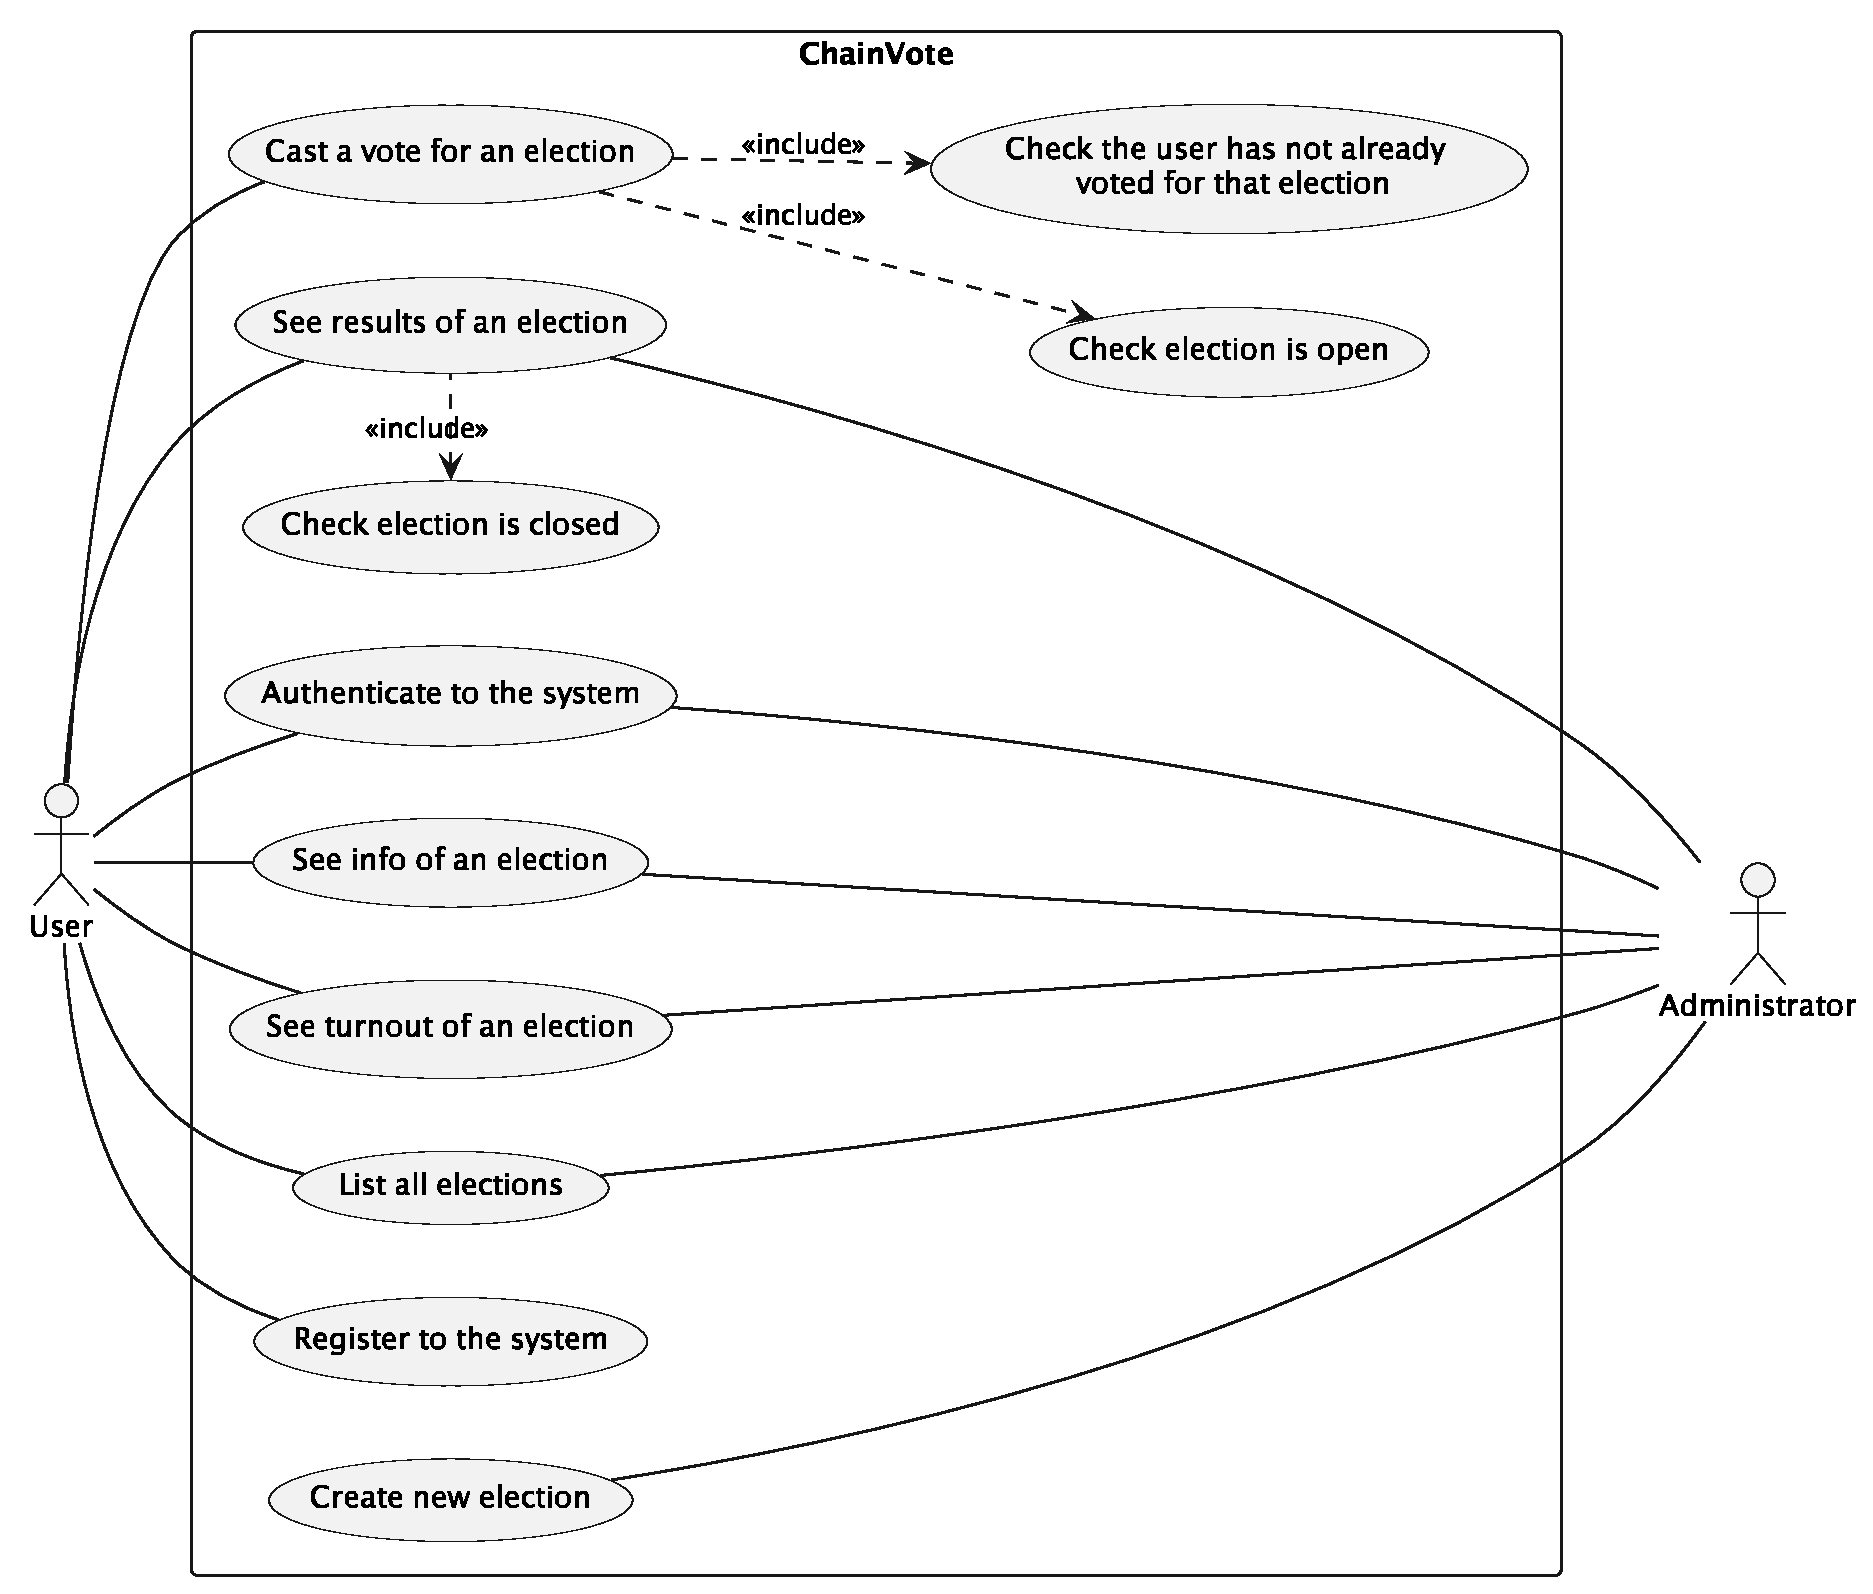
\includegraphics[width=\linewidth]{figures/use-cases.eps}
    \caption{Use cases diagram of the ChainVote application.}
    \label{fig:use-cases-diagram} 
\end{figure}

\subsection{Non functional requirements}
\label{sec:non-functional-requirements}

In order to decouple as much as possible users from their vote inside the blockchain and make it more difficult for unauthorized individuals to cast a vote impersonating someone else, \textbf{pseudo-random one-time codes} will be used.
%
The idea is that, before casting a new vote, the user requests a one-time code that is sent to him using a different trusted method.
%
When voting, the user will have to send back the generated one-time code to the system to correctly submit his vote.
%
The outline of use cases related to the casting of a vote in light of the above refinements is presented in \Cref{fig:refined-cast-vote-use-case}.

\begin{figure}
    \centering
    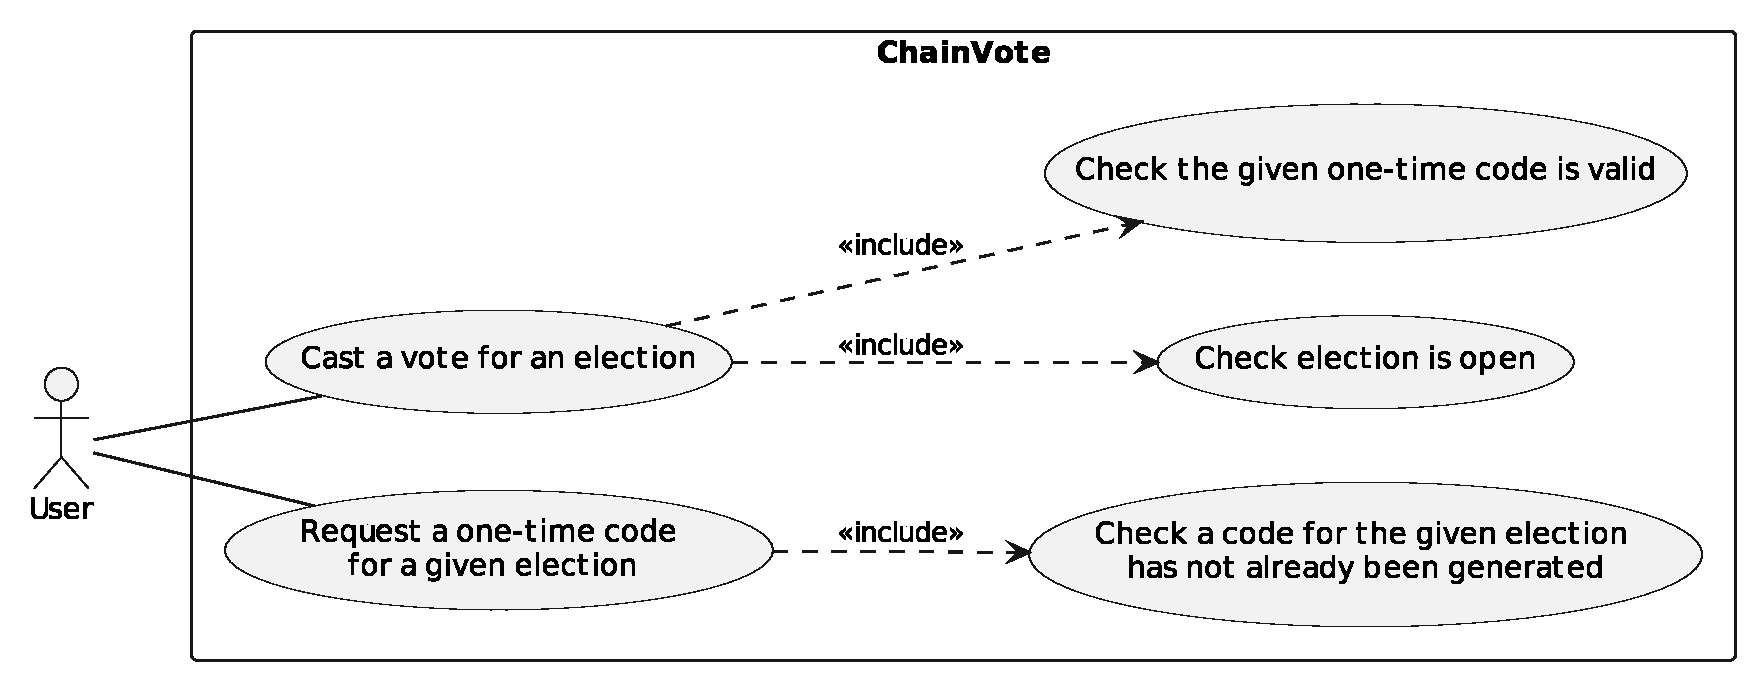
\includegraphics[width=\linewidth]{figures/refined-cast-vote-use-case.eps}
    \caption{Refined use case diagram for the casting of a vote.}
    \label{fig:refined-cast-vote-use-case}
\end{figure}

%% -------------------------------------- DS ----------------------------
\iffalse

To accomplish this, two challenges must be faced during the design process:

\begin{itemize}
    \item It is necessary that, within the ledger, the code-user association, as well as the expressed vote and user's code, are stored securely, i.e. are not recorded in clear in the blockchain bocks' transactions;
    \item Given that the deterministic nature of smart contracts makes it difficult to generate completely random codes, a deterministic algorithm will be used and a source of randomness will be injected from a trusted and controlled entity. It's worth mentioning their generation \textit{a priori} (i.e. when the election is created) is not feasible since smart contract transactions are executed by peers in any order, possibly even in parallel, implying that different peers may process the same client transaction with different order. This means that it is not possible to guarantee that, when the client triggers the transaction execution, peers will get the same code from the set of already generated ones.
\end{itemize}

\fi
%% -------------------------------------- DS ----------------------------

Moreover, for security reasons, the \textbf{user's password should not be stored in plain text} within the server storage, but password encryption mechanisms will have to be employed.

The web application must be designed to be accessible and have a user experience that allows even less experienced users to use it easily. For this, the design must be designed to be \textbf{responsive} and \textbf{mobile-first}. In addition, an important feature that must be supported is the responsiveness of the interface, which must be able to refresh and show voting-related information in \textbf{real-time} without having to refresh the page.

\subsection{Target User Analysis}

In order to meet the non functional properties concerning the user experience it's important to have a comprehensive understanding of our target audience.
%
In the next section is presented the target user analysis that serves as the compass guiding our decisions.

\subsubsection*{Admin users}

\noindent
\emph{%
    As an administrator (who), \\ 
    I want to create an election (what), \\ 
    So that interested users can express their vote (why).
}
\vspace*{0.2cm}

\textbf{Personas:} Alba

Alba is an administrator of the ChainVote system.

\textbf{Use Case Scenario:}

The University of Bologna needs to elect the next rector and wants to collect votes through the ChainVote system. Alba is tasked with creating the election.

\begin{enumerate}
    \item Alba logs into the platform using her credentials;
    \item Alba navigates to the "Create Election" section;
    \item Alba enters the election details:
    \begin{itemize}
        \item Estimated number of voters;
        \item Election start date;
        \item Election end date;
        \item Goal (election title);
        \item Choices.
    \end{itemize}
    \item Alba saves the election.
\end{enumerate}

\vspace*{0.5cm}
\noindent
\emph{%
    As an administrator (who), \\
    I want to view the election results (what), \\
    To make a decision regarding the consequences of the election (why).
}
\vspace*{0.2cm}

\textbf{Personas:} Giovanni

Giovanni is the rector of the University of Bologna.

\textbf{Use Case Scenario:}

Giovanni wants to view the results of the vote concerning the next rector of the University of Bologna so that he can congrats to him.

\begin{enumerate}
    \item Giovanni accesses the system with his credentials;
    \item Giovanni navigates to the "Dashboard" page;
    \item Giovanni selects the election with the goal "Next rector of UniBo";
    \item Giovanni verifies that the vote is closed;
    \item Giovanni views the results related to the election and the turnout.
\end{enumerate}

\subsubsection*{Users}

\noindent
\emph{%
    As a user (who), \\
    I want to access the system (what), \\
    To be able to use various functionalities (why).
}
\vspace*{0.2cm}

\textbf{Personas:} Luca

Luca is a university student in Engineering and Computer Science at the University of Bologna, Cesena campus.

\textbf{Use Case Scenario:}

Luca wants to connect to the system to view upcoming elections.

\begin{enumerate}
    \item Luca goes to the login page;
    \item Luca enters his username and password in the respective fields;
    \item Luca clicks the login button;
    \item Luca gets redirected to the Dashboard where all the elections are displayed.
\end{enumerate}

\vspace*{0.5cm}
\noindent
\emph{%
    As a user (who), \\
    I want to view system notifications (what), \\
    To stay updated (why).
}
\vspace*{0.2cm}

\textbf{Personas:} Deborah

Deborah is an out-of-town student. 

\textbf{Use Case Scenario:}

Deborah is waiting for the opening of the election and wants to receive and see a notification as soon as an election opens or is about to close.

\begin{enumerate}
    \item Deborah logs into the system with his credentials;
    \item Deborah views if there are new notifications from the navbar icon that signals not read notification;
    \item Deborah clicks on the navbar link that takes to the page related to her notifications;
    \item Deborah is notified by a toast popup if a notification is triggered by the server.
\end{enumerate}

\vspace*{0.5cm}
\noindent
\emph{%
    As a user (who), \\
    I want to request a one time code for an election (what), \\
    so that I can cast a vote for it (why).
}
\vspace*{0.2cm}

\textbf{Personas:} Oscar

Oscar is a member of the UniBo Council. 

\textbf{Use Case Scenario:}

Oscar wants to request a code to participate in the vote regarding the next rector of UniBo.

\begin{enumerate}
    \item Oscar logs into the system with his credentials;
    \item Oscar navigates to the "Dashboard";
    \item Oscar verifies that the election is open;
    \item Oscar accesses the code request area;
    \item Oscar clicks the button to request the code;
    \item Oscar views part of the code internally in a form on the page, and the other half is sent to his email address.
\end{enumerate}

\vspace*{0.2cm}
\noindent
\emph{%
    As a user (who), \\
    I want to cast a vote in an election (what), \\
    To express my preference (why).
}
\vspace*{0.2cm}

\textbf{Use Case Scenario:}

Oscar, after obtaining the code, wants to cast his vote.

\begin{enumerate}
    \item Oscar logs into the system with his credentials;
    \item Oscar navigates to the "Dashboard";
    \item Oscar verifies that the election is open;
    \item Oscar accesses the vote area;
    \item Oscar enters the code for the vote (previously obtained);
    \item Oscar chooses an option.
\end{enumerate}

\vspace*{0.2cm}
\noindent
\emph{%
    As a user (who), \\
    I want to view the results of an election (what),
    To understand the preferences expressed by users regarding the election (why).
}
\vspace*{0.2cm}

\textbf{Use Case Scenario:}

Oscar wants to view the results of the election.

\begin{enumerate}
    \item Oscar logs into the system with his credentials;
    \item Oscar navigates to the Dashboard;
    \item Oscar selects the election of his interest;
    \item Oscar verifies that the vote is closed;
    \item Oscar views the results related to the vote.
\end{enumerate}

\vspace*{0.5cm}
\noindent
\emph{%
    As a user (who), \\
    I want to change my password (what), \\
    So that I can access the system again (why).
}
\vspace*{0.2cm}

\textbf{Personas:} Aurora

Aurora is a kindly elderly person. 

\textbf{Use Case Scenario:}

Aurora wants to access the system after a long period and realizes she has forgotten the login password for her account.

\begin{enumerate}
    \item Aurora connects to the login page;
    \item Aurora clicks the "recover password" link;
    \item Aurora enters her information (email) and clicks the "Recover Password" button;
    \item Aurora receives instructions to reset the password at the email address provided in the previous step;
    \item Aurora logins again into the system.
\end{enumerate}

\section{Design}

This section present the overall design of the system, both frontend and backend side.

\subsection{Frontend design}

\subsubsection*{Mockups}

Style in a web application is an important aspect to consider to fulfill usability requirements described above.
%
In order to devise a design that would enable a good user experience of the final product, initial mockups had to be carried out. 

As already specified in the non-functional requirements, design of the application is mobile-first. 
%
This means that mockups have been made and thought out in their elements primarily in the mobile context and adapted to be usable in a user-friendly manner and taking advantage of all the spaces available in the desktop version.

The only page accessible by unauthenticated users is the home page where is described the purpose of the project.

The user, in order to use the system, is required to log in (\Cref{fig:login-dashboard-elections-views}).
%
Once correctly logged, the user is redirected to the Dashboard where all the elections are displayed, categorized by "Open", "Closed" and "Soon".

Reasoning about usability, has been decided to add another view, Election view, where elections can be displayed, rather categorized or unfiltered. Moreover, vertical display allows a smoother visualization, up to 10 per page even in mobile setting.
%
From both visualization views, users can see the details of an election (\Cref{fig:details-cast-notifications-view}), ask for the code required during voting phase and reach the page to cast a new vote.
%
From the navbar is possible to navigate the notifications view where all recent notifications are displayed along with an indication of whether it has already been read or not.

\begin{figure}[h]
    \centering
    \begin{subfigure}[b]{0.3\textwidth}
        \centering
        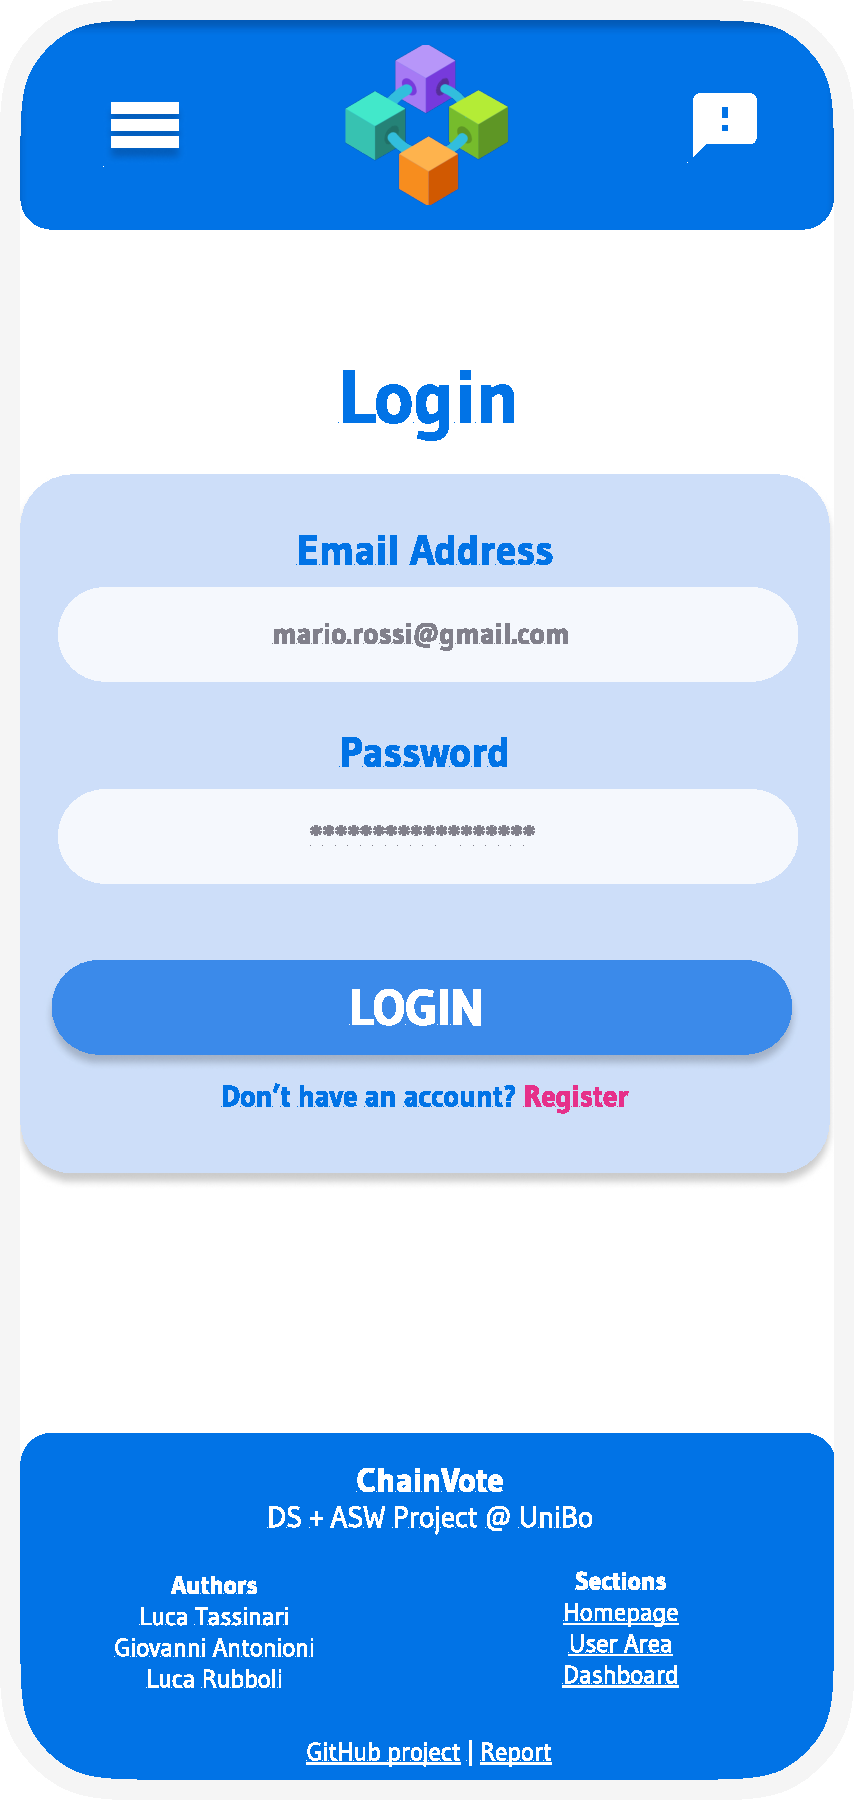
\includegraphics[width=\textwidth]{./figures/mockups/login.pdf}
    \end{subfigure}
    \hfill
    \begin{subfigure}[b]{0.3\textwidth}
        \centering
        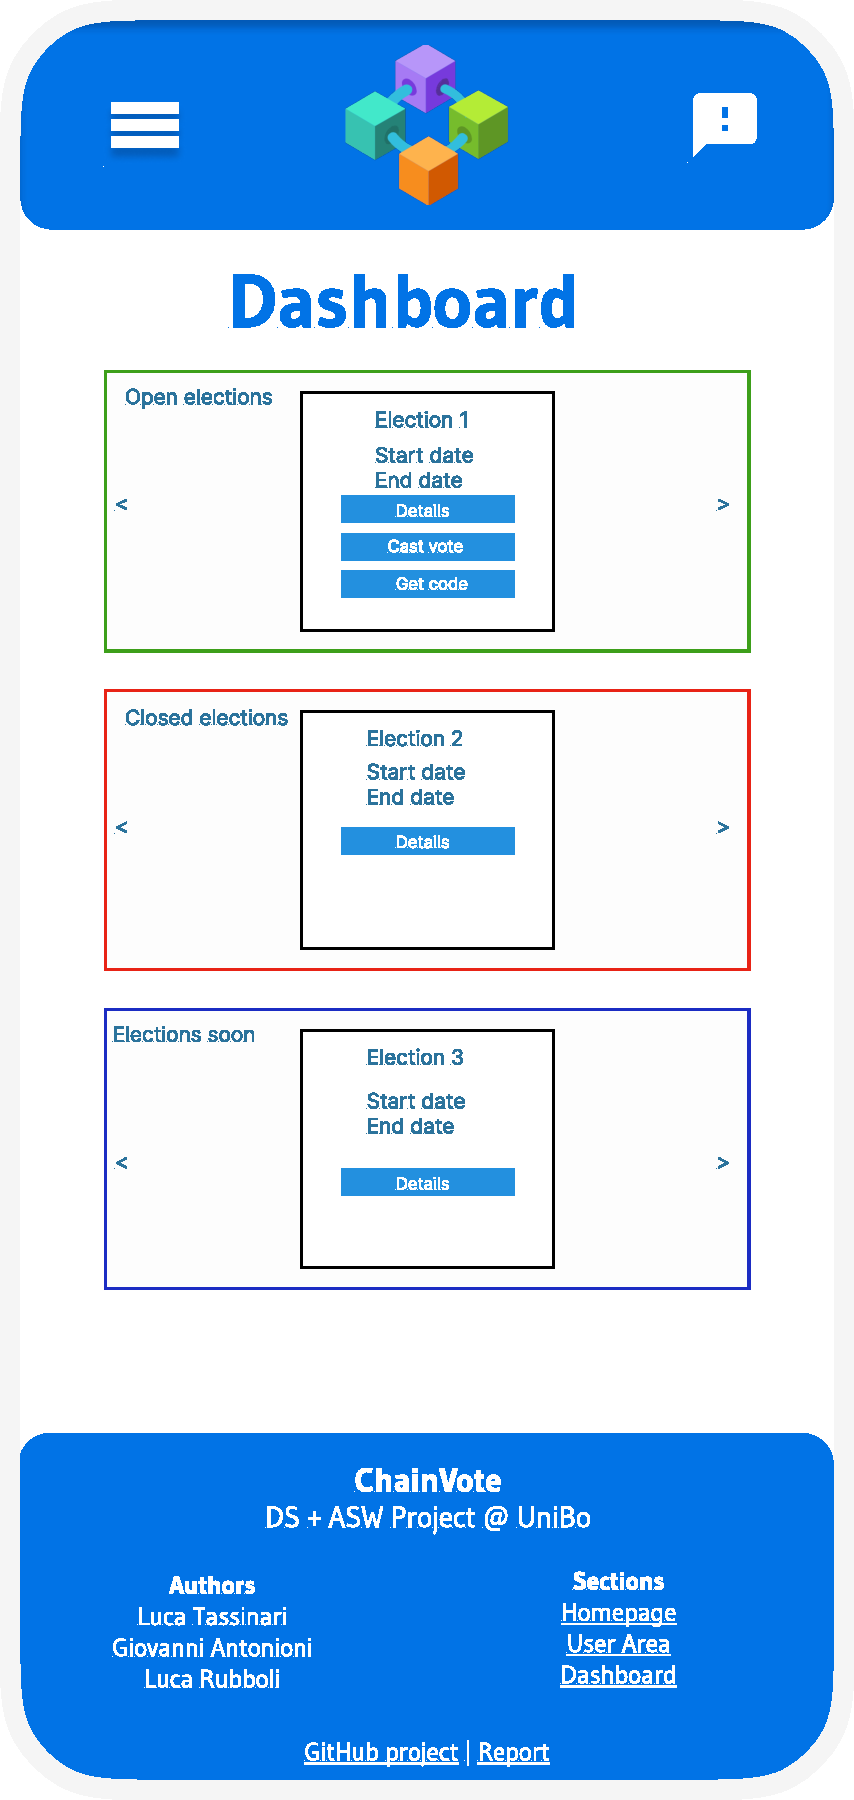
\includegraphics[width=\textwidth]{./figures/mockups/dashboard.pdf}
    \end{subfigure}
    \hfill
    \begin{subfigure}[b]{0.3\textwidth}
        \centering
        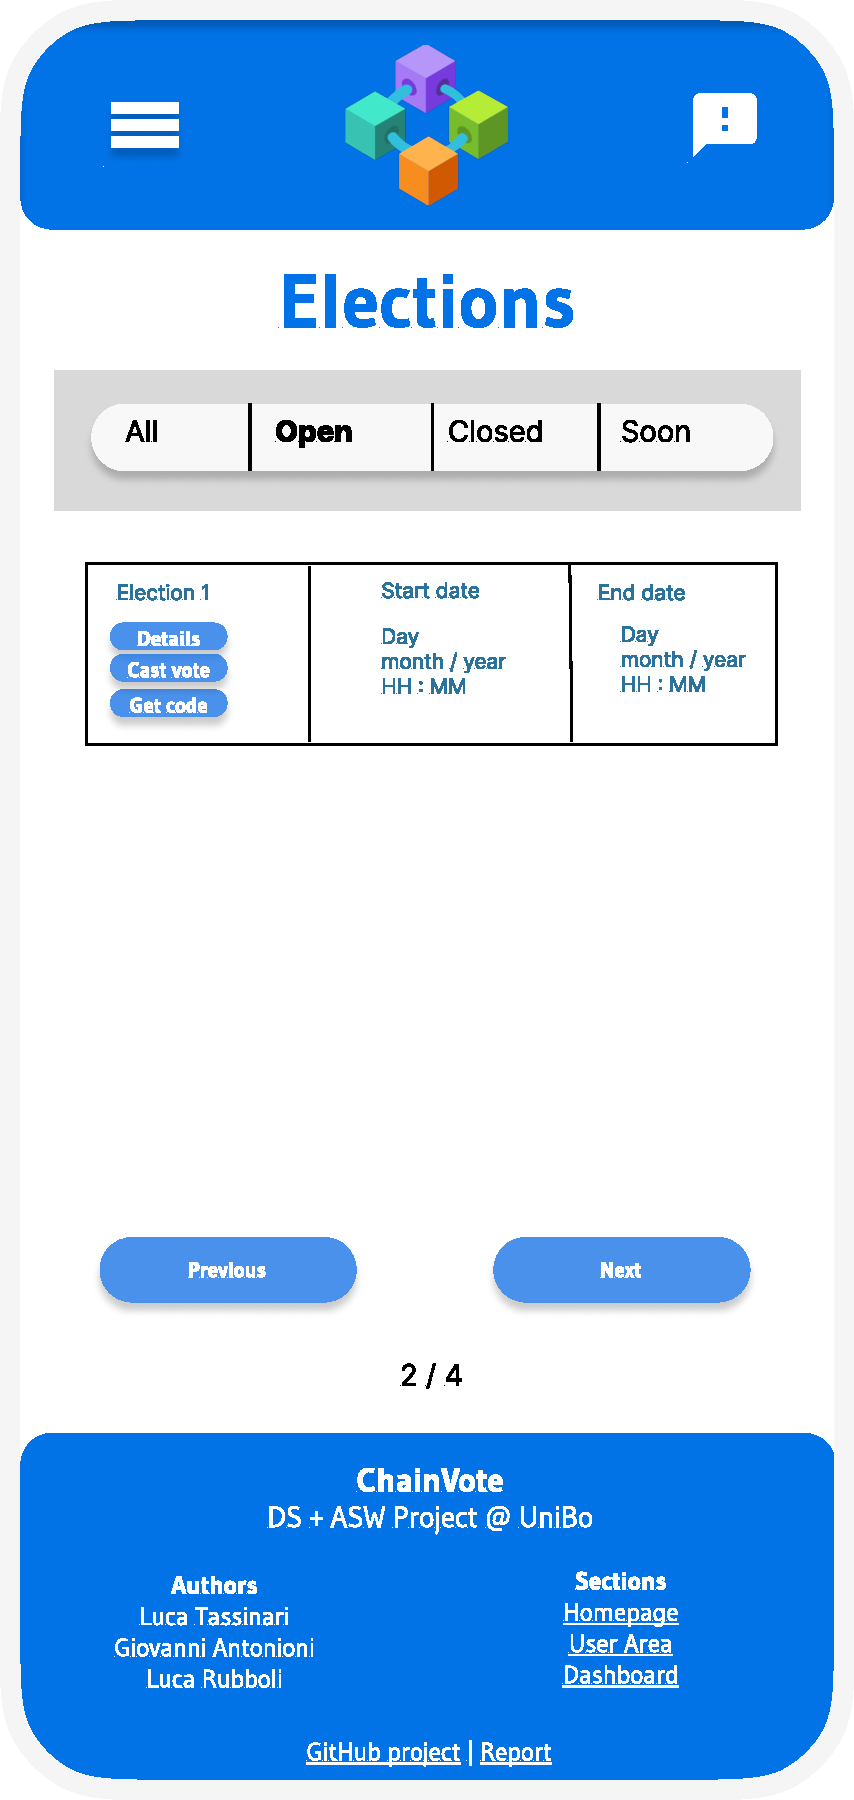
\includegraphics[width=\textwidth]{./figures/mockups/elections.pdf}
    \end{subfigure}
    \caption{Login, Dashboard and Elections views}
    \label{fig:login-dashboard-elections-views}
\end{figure}

\begin{figure}[h]
    \centering
    \begin{subfigure}[b]{0.3\textwidth}
        \centering
        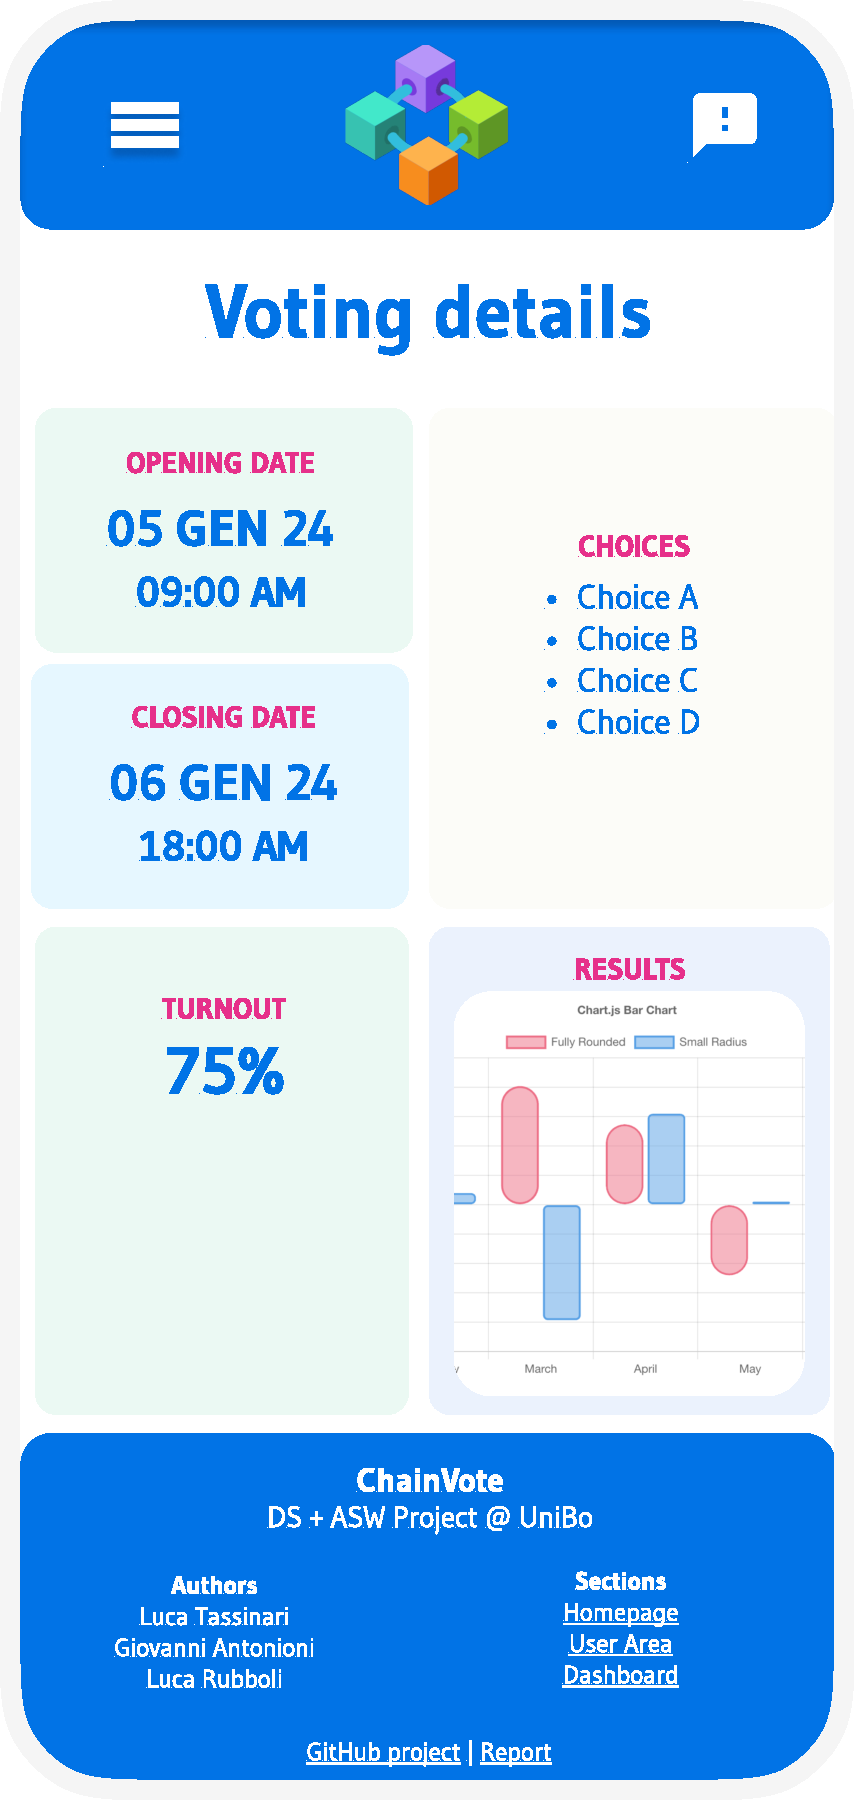
\includegraphics[width=\textwidth]{./figures/mockups/details.pdf}
    \end{subfigure}
    \hfill
    \begin{subfigure}[b]{0.3\textwidth}
        \centering
        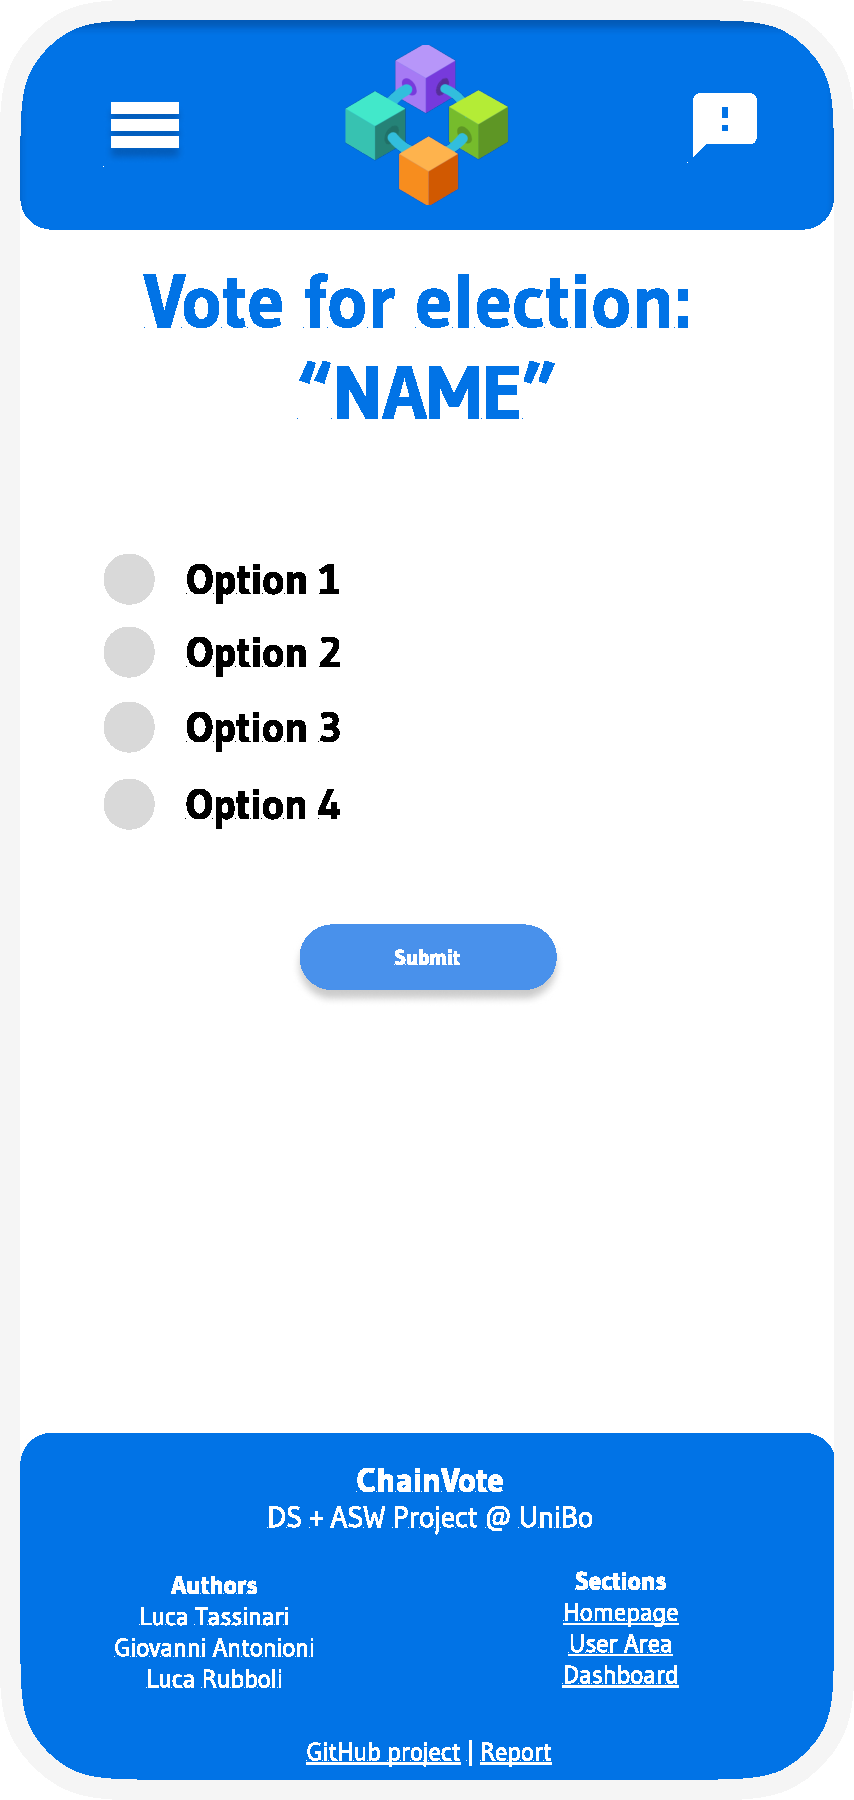
\includegraphics[width=\textwidth]{./figures/mockups/vote-page.pdf}
    \end{subfigure}
    \hfill
    \begin{subfigure}[b]{0.3\textwidth}
        \centering
        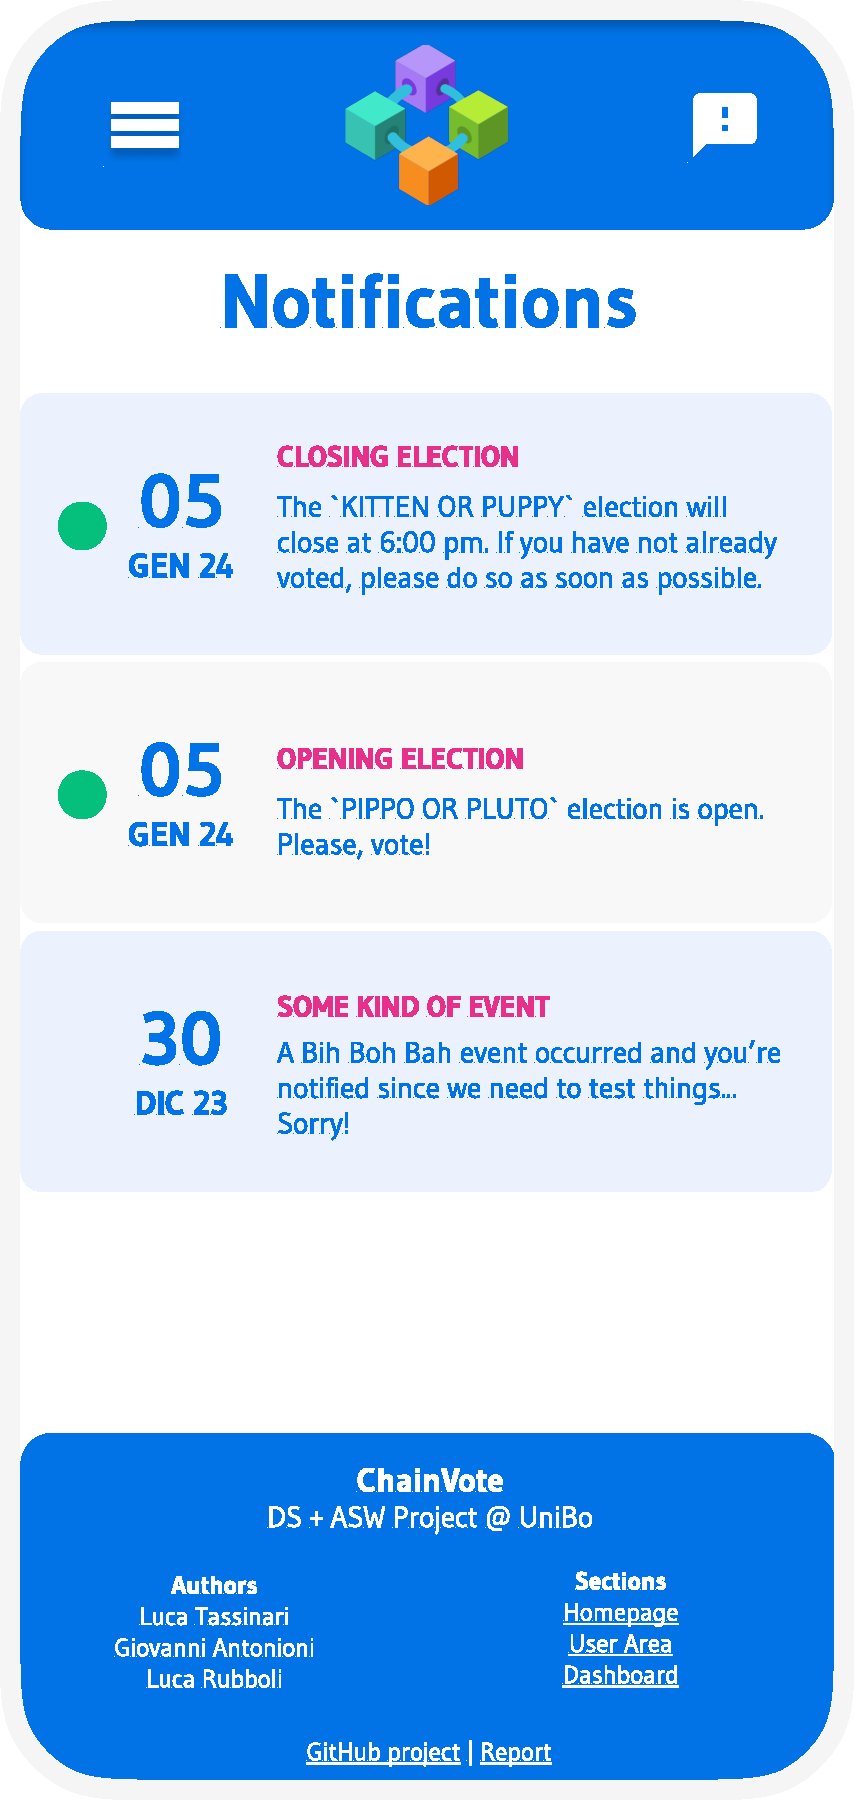
\includegraphics[width=\textwidth]{./figures/mockups/notifications.pdf}
    \end{subfigure}
    \caption{Voting details, Cast a vote and Notifications view.}
    \label{fig:details-cast-notifications-view}
\end{figure}

\begin{figure}[h]
    \begin{subfigure}[b]{0.3\textwidth}
        \centering
        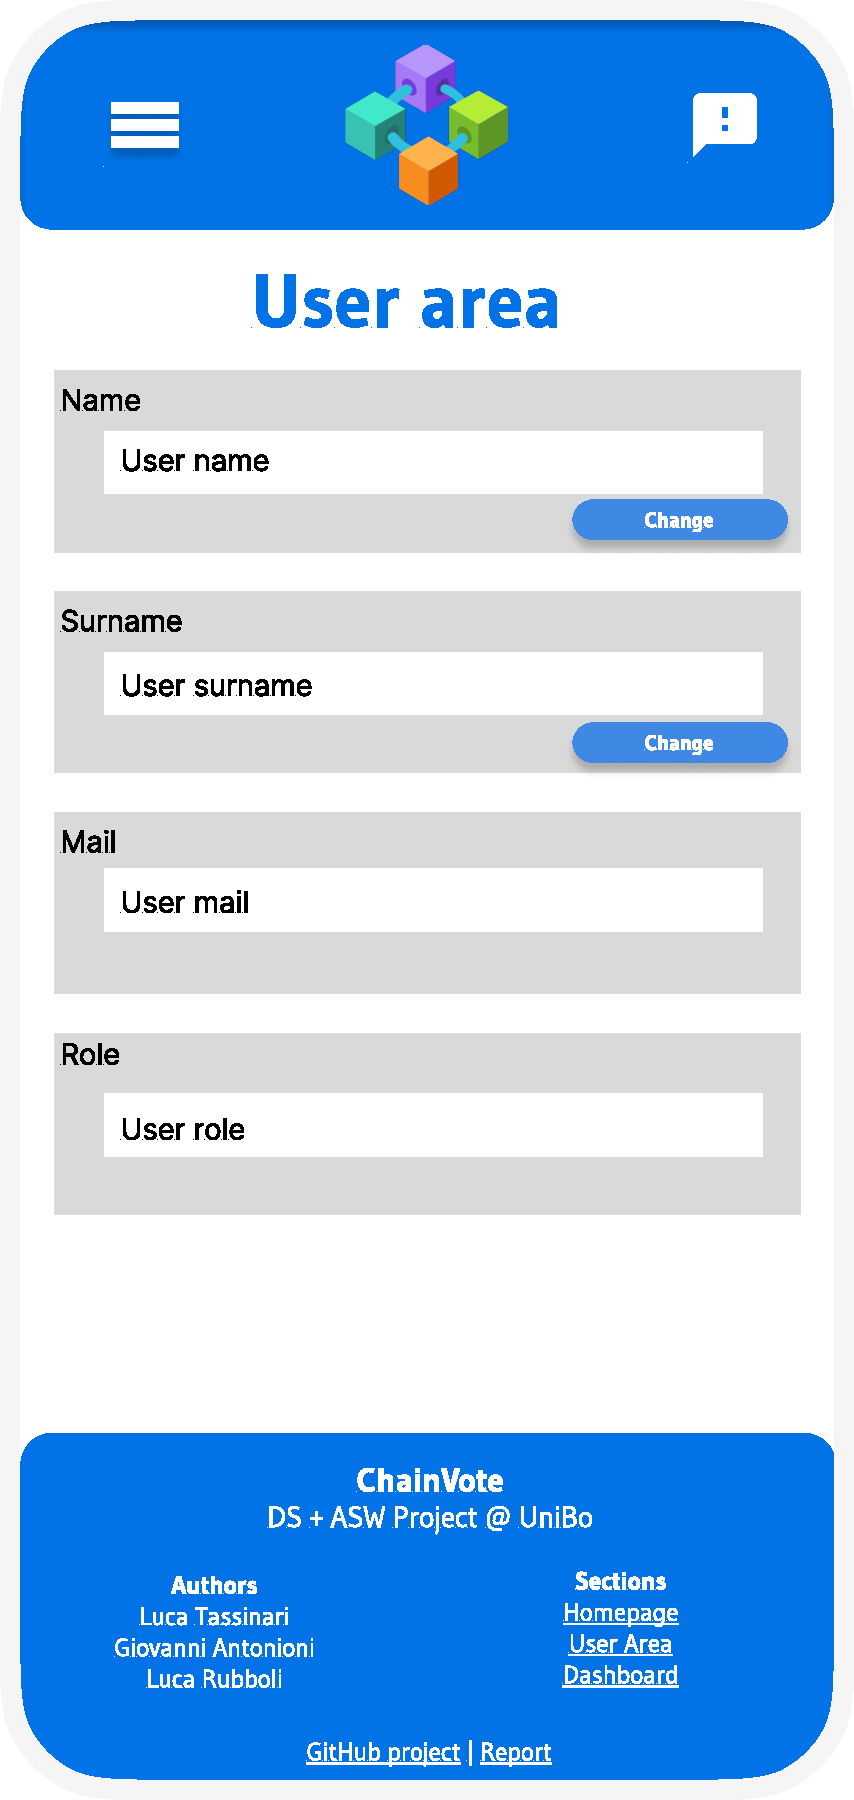
\includegraphics[width=\textwidth]{./figures/mockups/user-area.pdf}
    \end{subfigure}
    \hfill
    \begin{subfigure}[b]{0.3\textwidth}
        \centering
        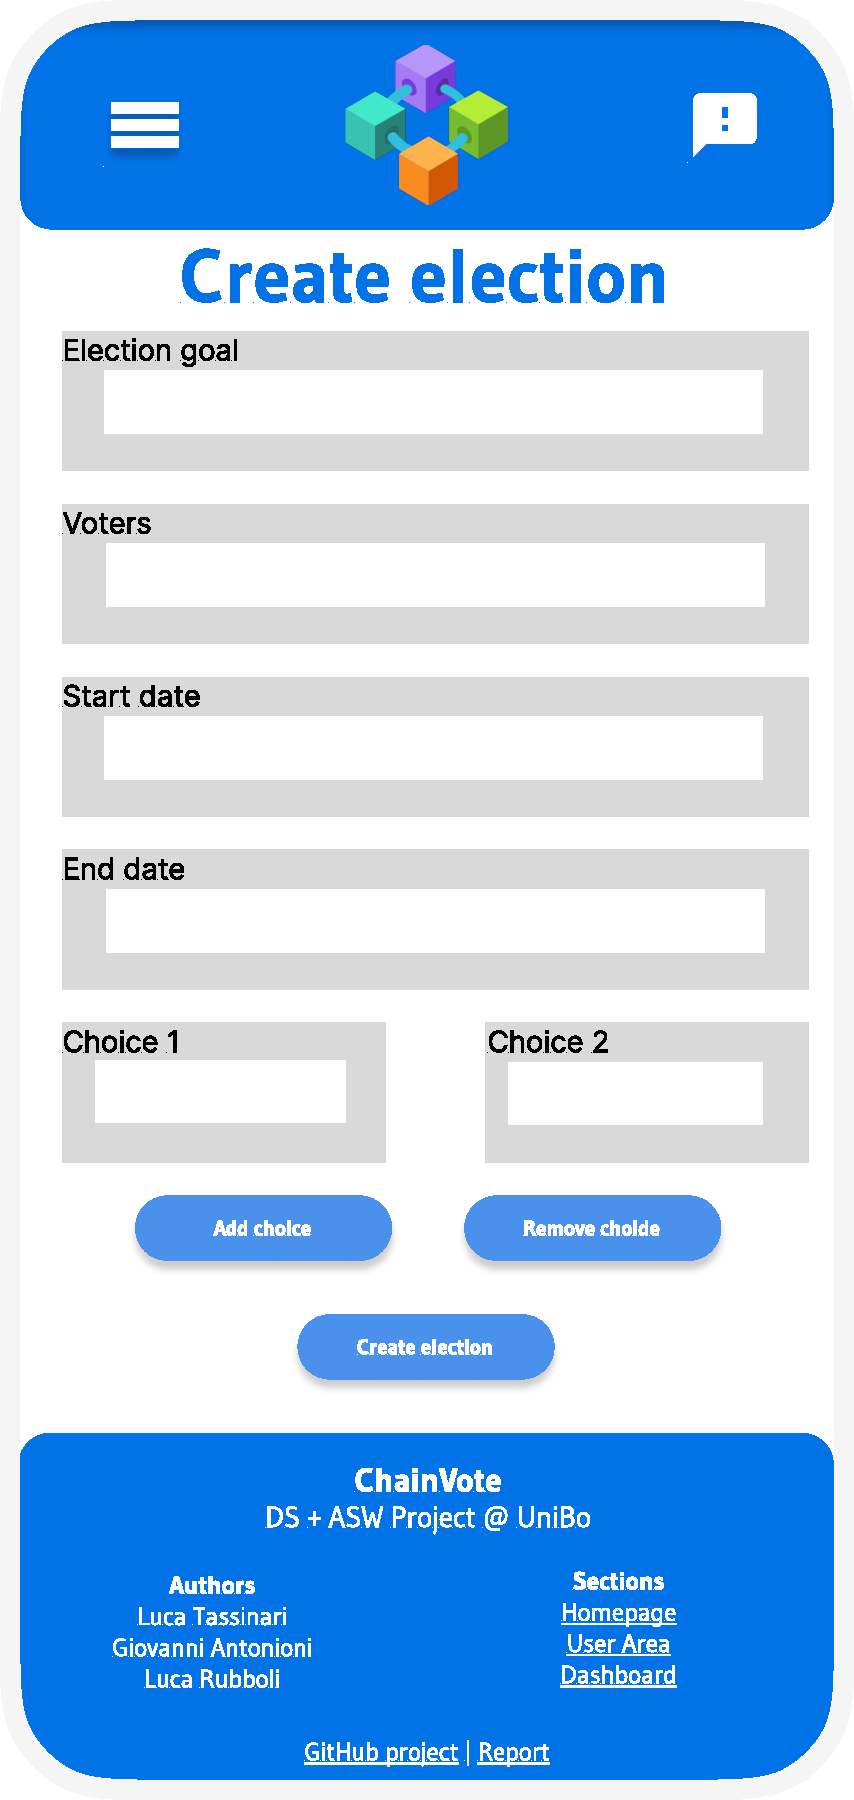
\includegraphics[width=\textwidth]{./figures/mockups/create-election.pdf}
    \end{subfigure}
    \hfill
    \begin{subfigure}[b]{0.3\textwidth}
        \centering
        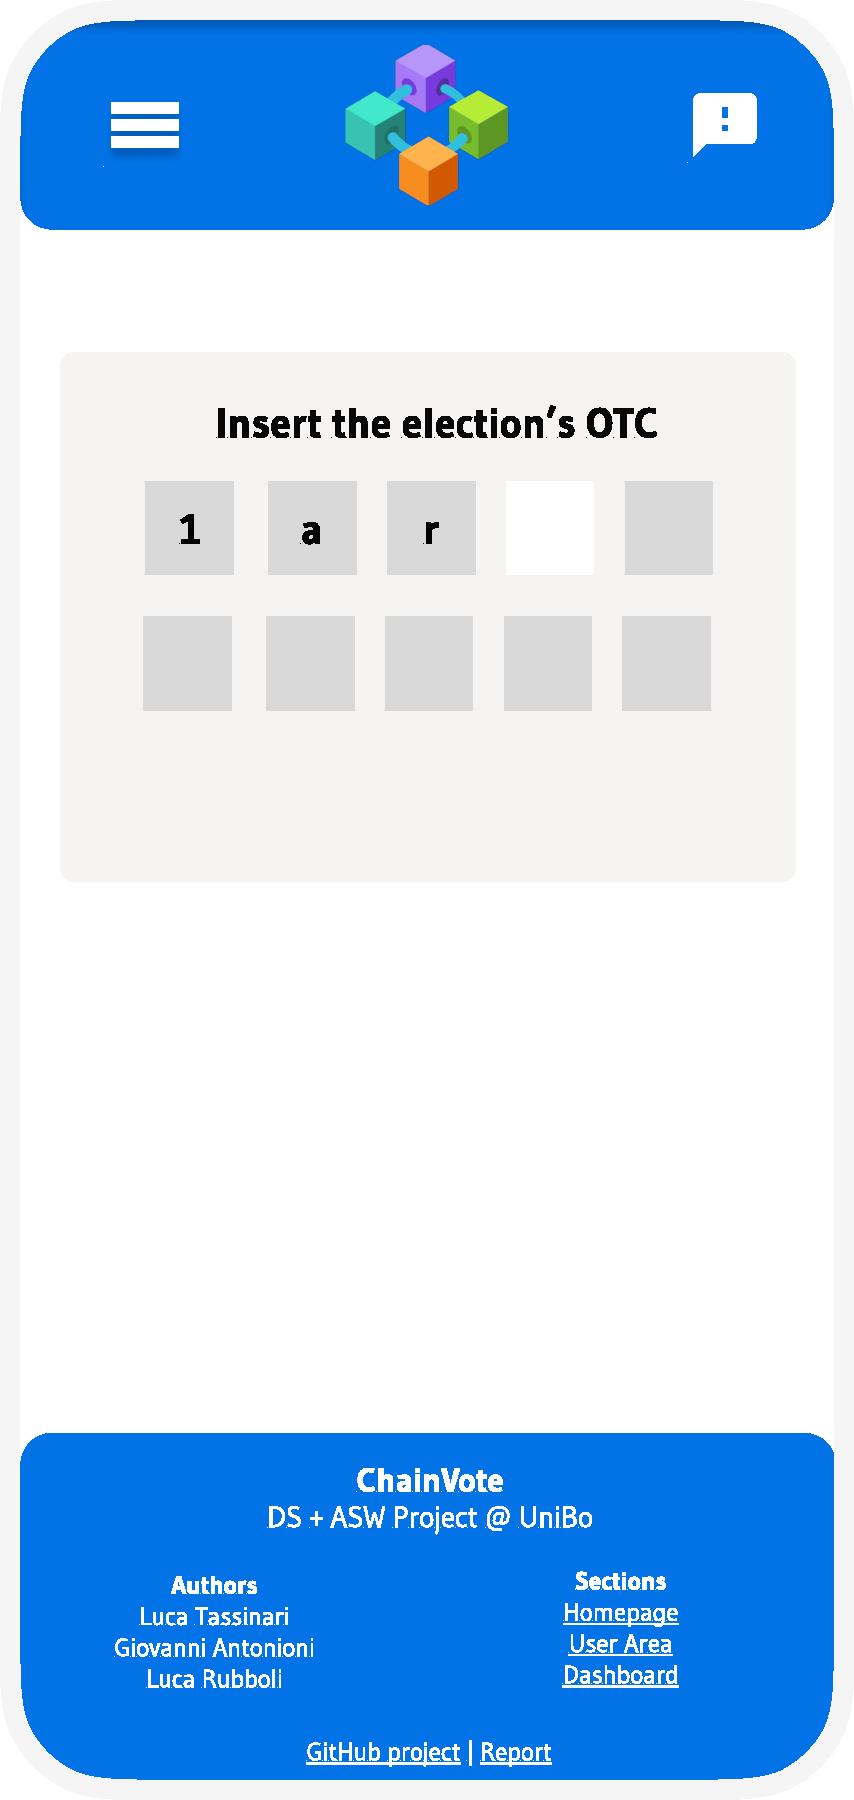
\includegraphics[width=\textwidth]{./figures/mockups/otc.pdf}
    \end{subfigure}
    \caption{User area, Create election and OTC request view.}
    \label{fig:user-area-view}
\end{figure}

\subsection{Backend Architecture}
The following section presents the overall architecture of the system's backend that is principally composed  by two modules:
\begin{itemize}
    \item Blockchain network: based on Hyperledger Fabric, maintains the business logic regarding votes and elections;
    \item API server: used as middleware between the blockchain network and the clients, it exposes the API to interact with the system
\end{itemize}

Focusing on the API server module shown in \Cref{fig:system-architecture}, we can see that it provides its functionality through the \texttt{:api-server} and \texttt{:auth-server} submodules: \texttt{:api-server} maintains the logics for interacting with the blockchain network, manage the users data and send the events to the frontend using websockets. \texttt{:auth-server} exposes the login endpoints and generates the JWT tokens used to authenticate the users.

Both modules are based on the same technological stack (Node and Express.js) and share some common functionality distributed through the use of an internal dependency registry (represented as \texttt{:common} in \Cref{fig:system-architecture}). The utility classes and functions are packed as a npm package and imported as dependency.

Other than the blockchain's ledger the system relies on two databases, both contained in the \texttt{:api-service} module:
\begin{itemize}
    \item \texttt{MongoDB} stores persistent information, i.e., user data and authentication tokens.
    \item \texttt{Redis} is used for storing temporary data, i.e., the number of requests for a specific endpoint.
\end{itemize}

Clients can also receive notifications from the server through the use of websockets. The server uses the \texttt{socket.io} library to send events to the clients.

\newgeometry{margin=1.0cm}
\begin{landscape}
    \begin{figure}
        \centering
        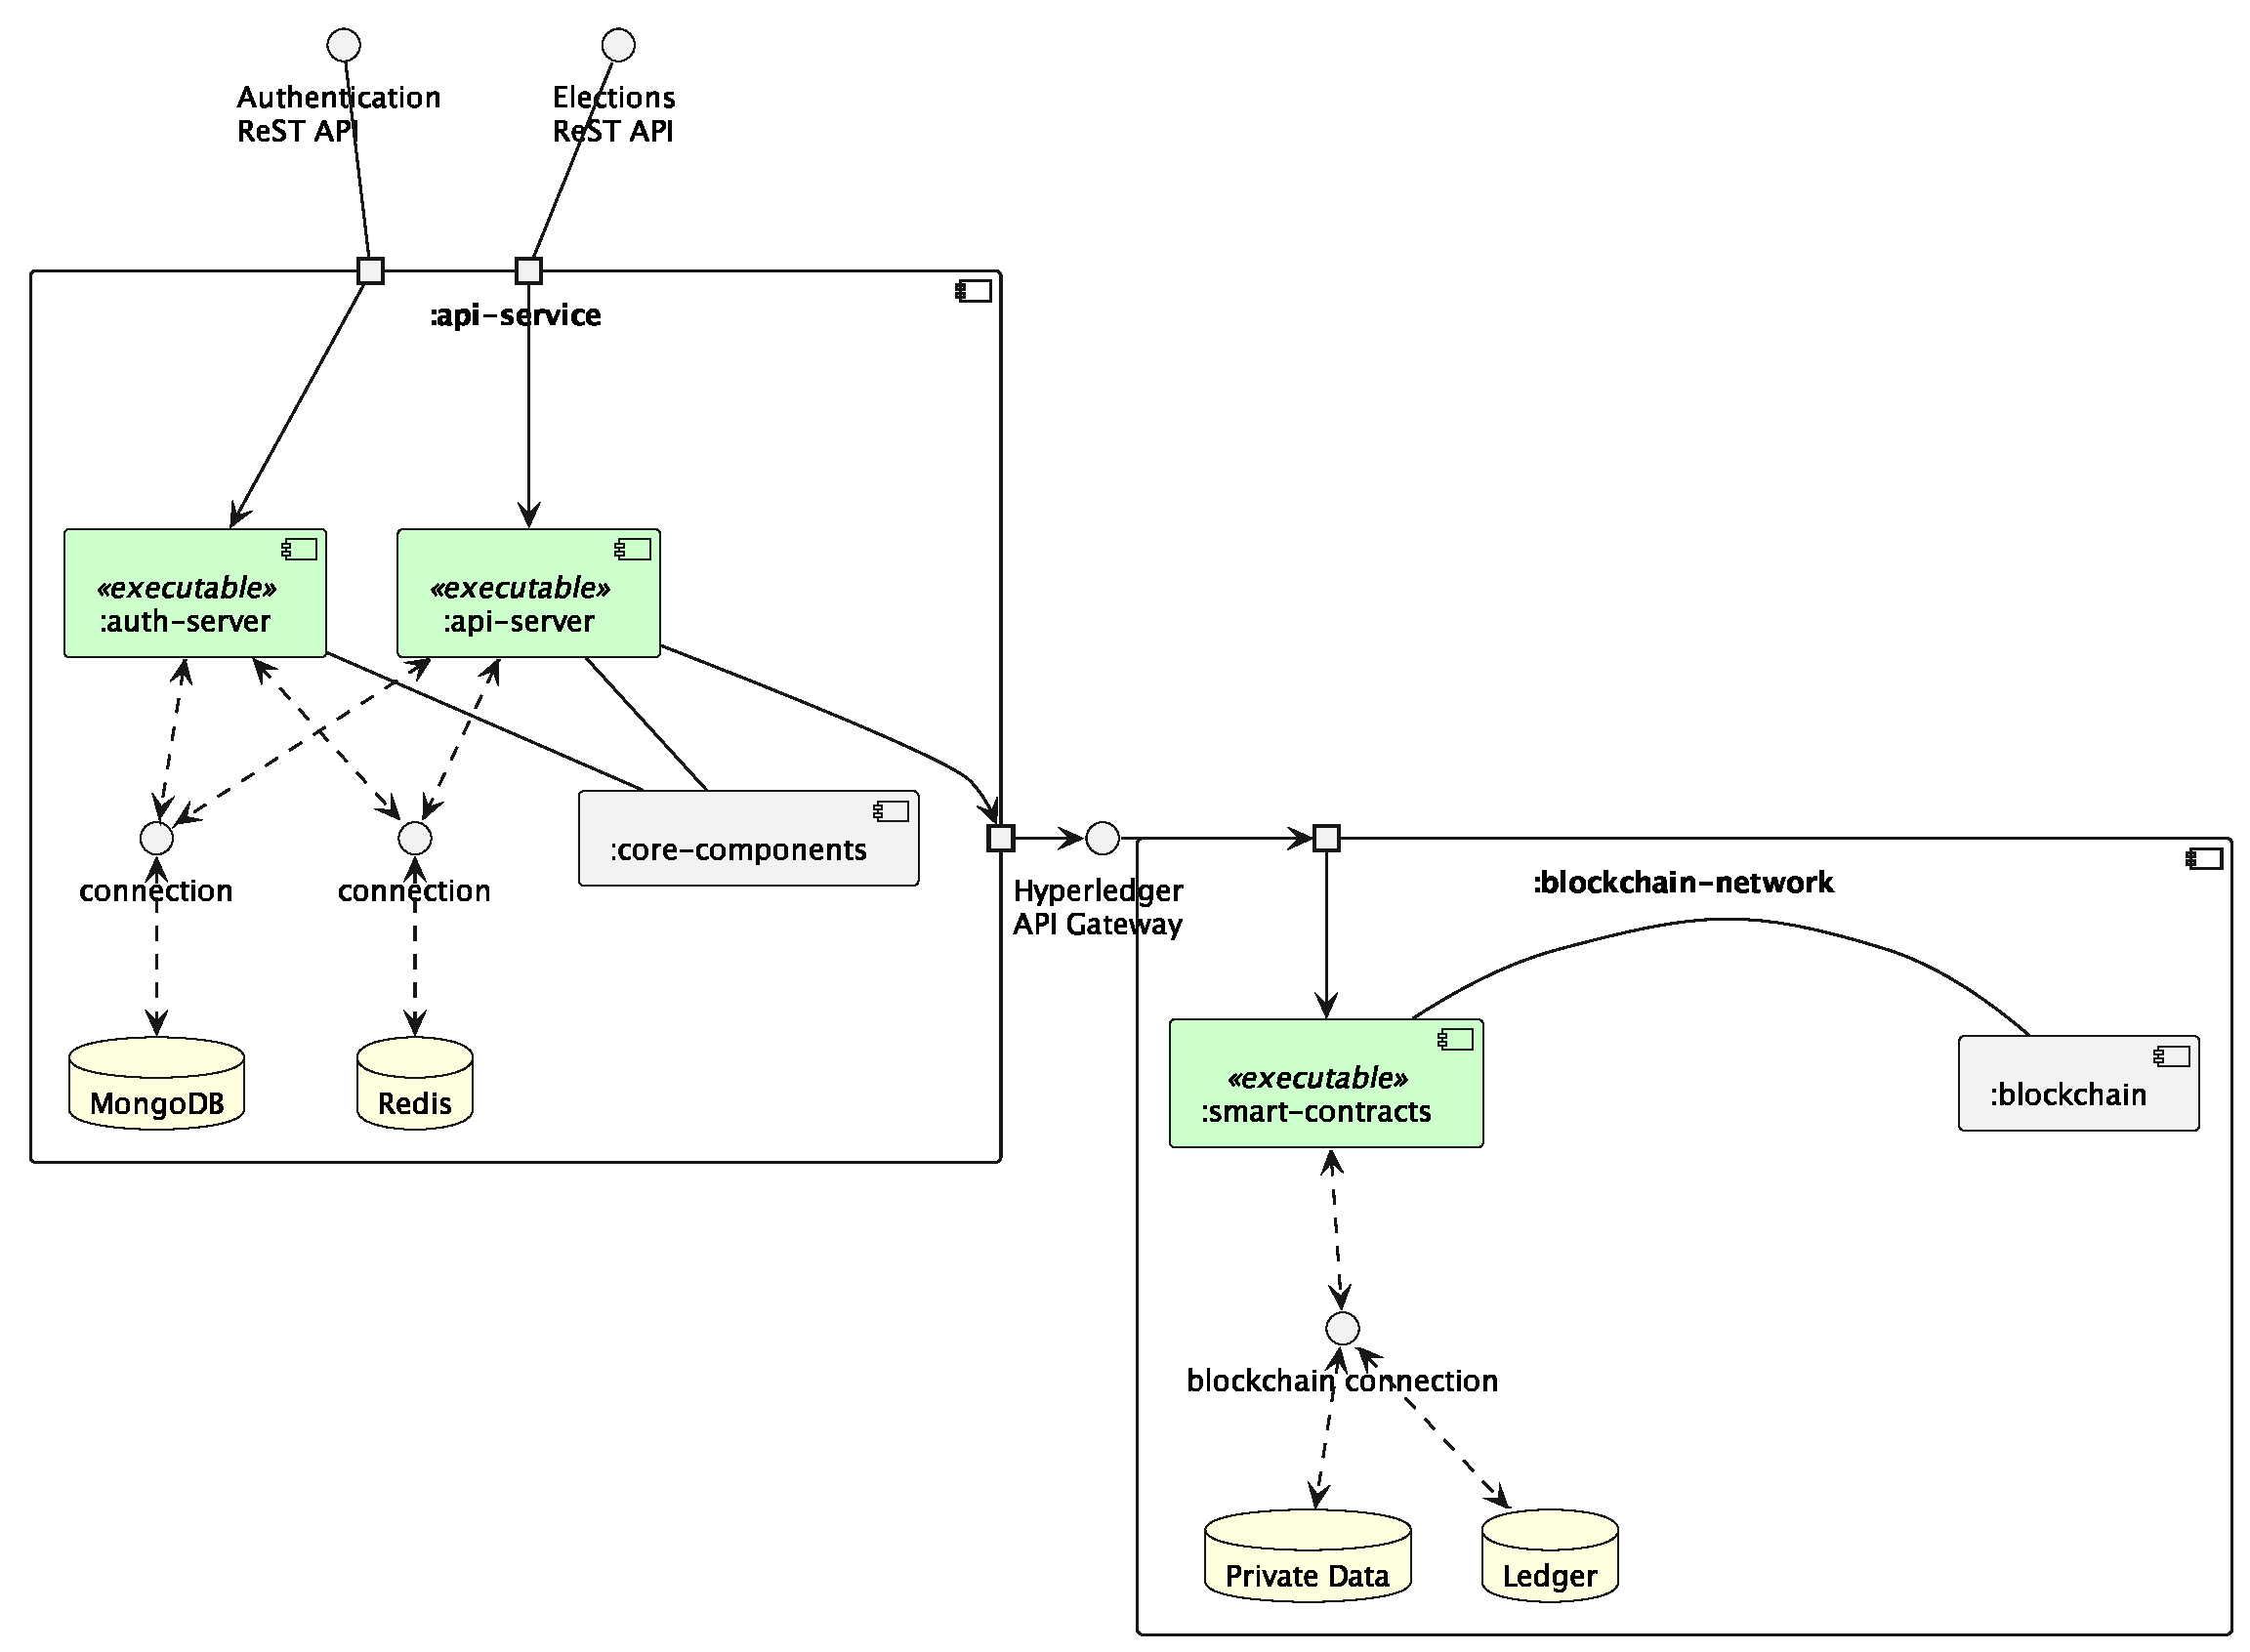
\includegraphics[width=0.7\linewidth]{figures/system-architecture.eps}
        \caption{UML class diagram of the election's domain entities.}
        \label{fig:system-architecture} 
    \end{figure}
\end{landscape}
\restoregeometry

\subsection{Technologies}
\label{sec:technologies}

As solution stack, we've adopted \texttt{MEVN}, in detail
\begin{itemize}
    \item \texttt{Node} and \texttt{Express} server side;
    \item \texttt{Vue} client side;
    \item \texttt{MongoDB} as storage technology;
    \item \texttt{mongoose} for DB interactions;
    \item \texttt{Redis} as caching storage;
    \item \texttt{Socket.io} to achieve real-time updates;
    \item \texttt{Verdaccio} as internal repository system;
    \item \texttt{Axios} to deliver asynchronous HTTP requests;
    \item \texttt{npm} as dependency manager;
    \item \texttt{Hyperledger Fabric} as open source Blockchain framework;
    \item \texttt{Docker} as virtualization system manager and to smooth deployment.
\end{itemize}

Moreover, we used the following languages
\begin{itemize}
    \item \texttt{Java} as main blockchain's chaincode language;
    \item \texttt{Typescript}, both server and client side;
    \item \texttt{HTML} as views' structure;
    \item \texttt{CSS} and \texttt{SCSS} as style sheets.
\end{itemize}

During development we got in touch with minor technologies, it's worth mentioning \texttt{Swagger OpenAPI}, by means of which we documented our RestAPI and \texttt{bootstrap} to enhance page style.

\section{Implementation Details}

\subsection{API Server}

\subsubsection{Authentication}
Authentication within the system is implemented by the use of \texttt{JWT tokens}. JWT \cite{jwt} is an open standard that allows the secure transmission of information between two parties as a JSON object. The information passed is digitally signed using the RS256 algorithm so it can be trusted and verified by an entity that requests it. Both the sign and verify functions for an access token are distributed to the \texttt{API} and \texttt{AUTH} server inside the \texttt{:common} package.

When a user tries to log in, the \texttt{AUTH} server will sign an access and a refresh token. The first one has a validity of 15 minutes while the latter one of 30, both will be securely signed by a private key and then sent back to the client. 

\jsimport[
    caption={The login method in the auth server},
    label={lst:login-auth-server}
]{listings/login.ts}

The client is responsible for securely storing the tokens and for sending them to the request that requires authentication. Before accessing the routes, \texttt{API} server verifies the validity of the access token and extract 
the information that it needs from it.
This operation is performed by a middleware that is executed before the request is processed by the route handler. It verifies the validity of the token and extracts the information that it needs from it. If the token is valid, the middleware registers the user information and sends it to the function that handles the request. If the token is not valid, the middleware sends back an error response.

\jsimport[
    caption={The middleware that handles the authentication},
    label={lst:auth-middleware}
]{listings/authentication.handler.ts}

\begin{figure}
    \centering
    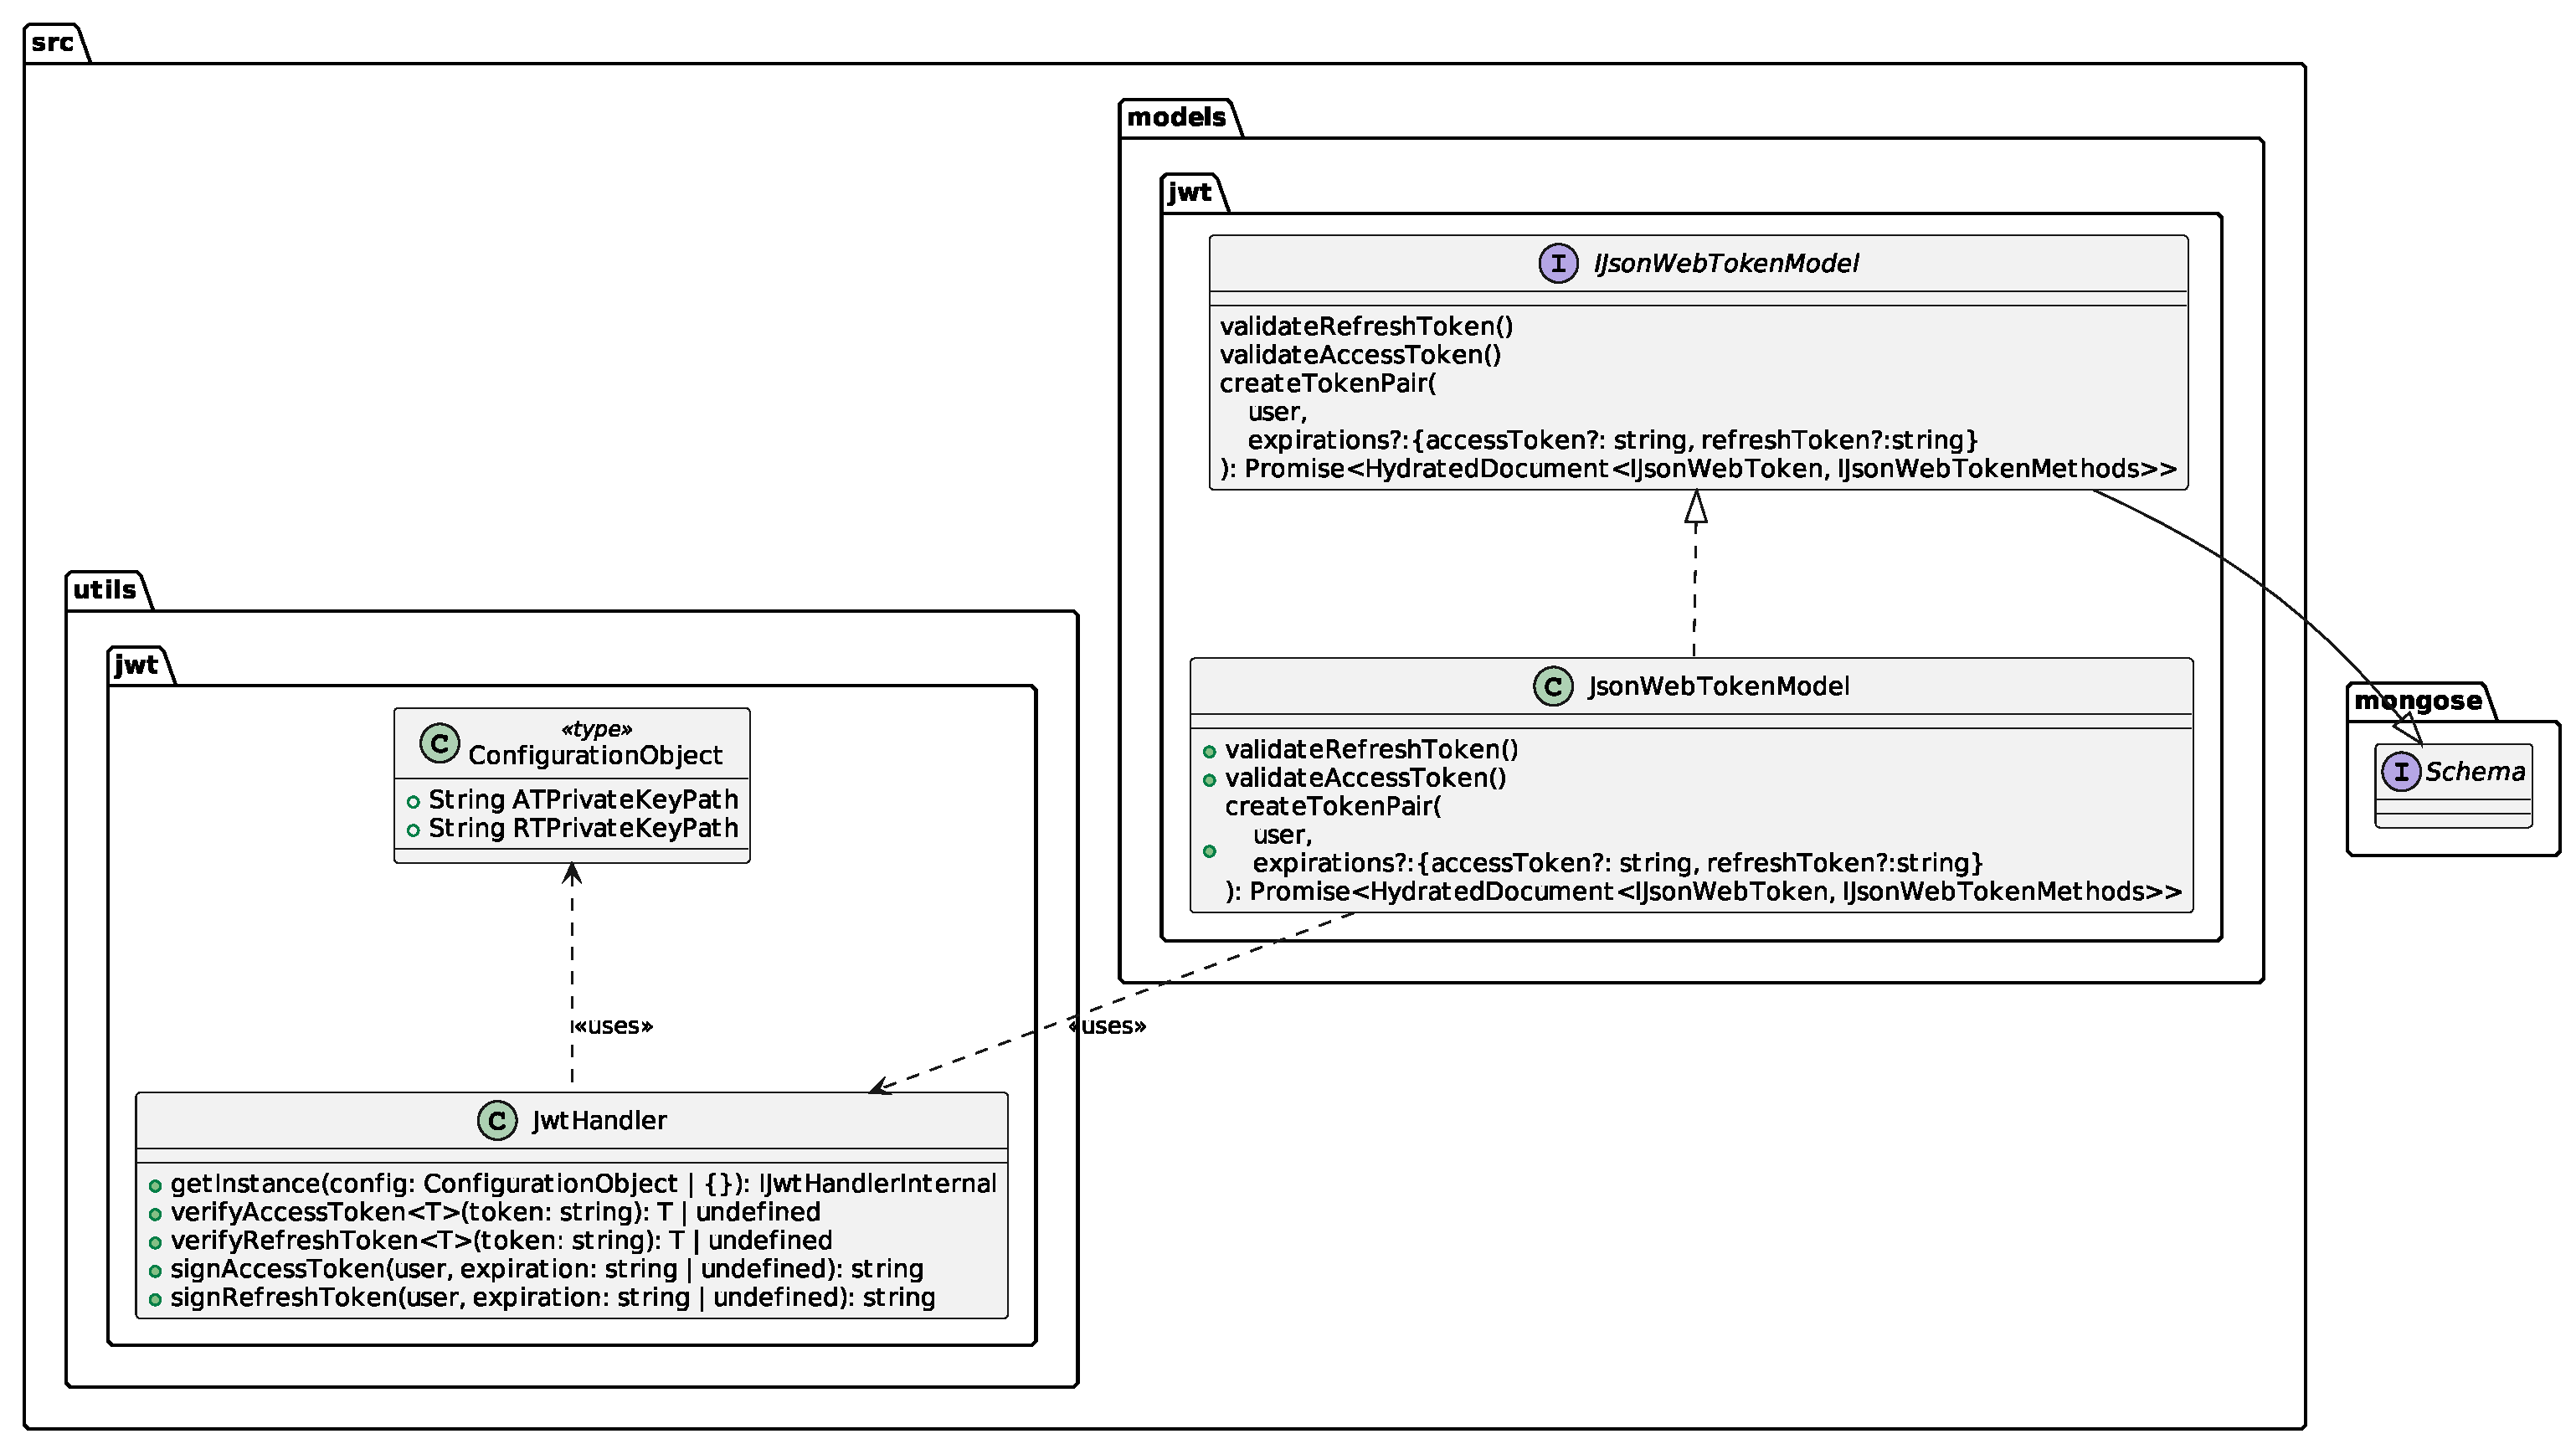
\includegraphics[width=\linewidth]{figures/jwt-api.eps}
    \label{fig:jwt-packages-api} 
    \caption{The overall API for the management of the JWT tokens}
\end{figure}

The \texttt{Jwt} model handles the verification and persistence of tokens inside the \texttt{MongoDB} database. It uses the namesake utility class, located within the \texttt{utils.jwt} package which is responsible for managing the construction of the various parts of the token.

\begin{warn}[\textit{Warning}]
    Once the network is deployed, the script copies a pair of public \& private keys in \texttt{api}, \texttt{auth} and \texttt{common} modules. While this operation simplifies the deployment process, and its testing, we're aware that in a real scenario, this would be a security issue and the private key should be stored and distributed relying on a more secure way.
\end{warn}

\subsubsection{Rate limiter}
We've implemented a custom rate-limiter module inside the API layer, which is responsible for limiting the number of requests that a client can send to a specific endpoint. This is done by using a \texttt{Redis} database that stores the number of requests that a client has sent to a specific endpoint. The rate limiter is implemented as a middleware that is executed before the request is processed by the route handler. It checks if the client has exceeded the maximum number of requests allowed, if so it sends back an error response to the client, otherwise, it increments the number of requests and sends the request to the route handler.

The way it works is as follows: each controller specifies a set of rules for each endpoint that can vary from the type of request.

\jsimport[
    caption={The definitions of the rules for the rate-limiter},
    label={lst:rate-limiter-rules}
]{listings/api.rule.ts}

In \Cref{lst:rate-limiter-rules} we listed the rules for three endpoints, each of them specify for the \texttt{verb} type two parameters:
\begin{itemize}
    \item \texttt{time}: The time window in which the requests are counted.
    \item \texttt{limit}: The maximum number of requests that can be sent in the specified time window.
\end{itemize}

So, for example, \texttt{endpoint\_name\_1} can receive a maximum of 50 requests in 18 seconds if the request type is \texttt{POST} and 60 requests in 14 seconds if the request type is \texttt{GET}.
The set of rules is then passed to the RateLimiter middleware which retrieves the IP address of the client and the endpoint that is being requested. 
Route checking is done on data saved on a \texttt{Redis} database. To make this solution more modular and extensible a Storage (\texttt{ApiLimiterStorage}) interface was devised that defines the operations to be performed on the data. 

\jsimport[
    caption={The limiter middleware},
    label={lst:rate-limiter-middleware}
]{listings/api.limiter.ts}

\begin{figure}
    \centering
    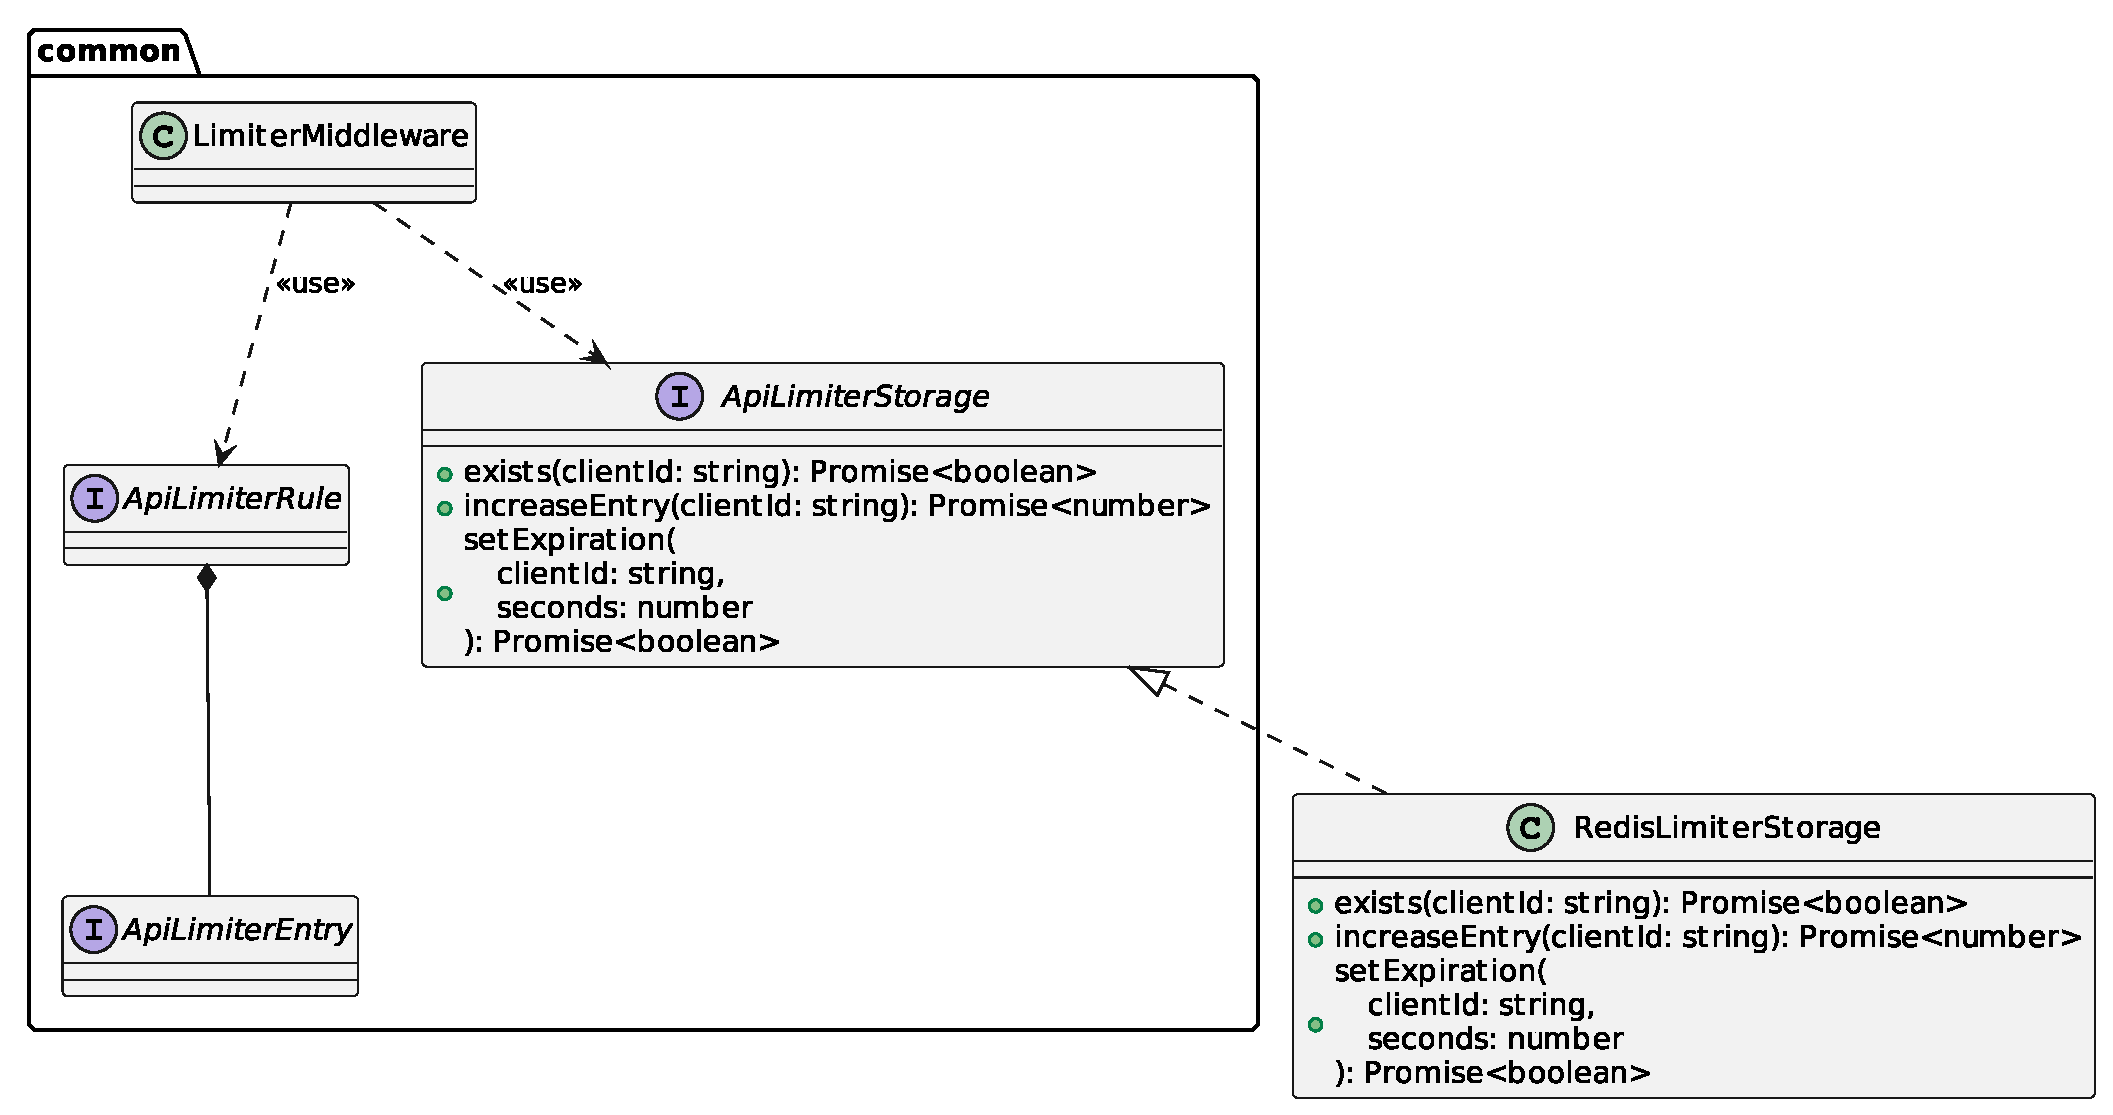
\includegraphics[width=\linewidth]{figures/api-limiter-api.eps}
    \label{fig:api-limiter-api} 
\end{figure}

\subsubsection{Mailer}
The system can send emails to the user by the means of a mailer component configured inside the API server. 
We use a custom gmail account which credentials are passed using a docker secret on the initialization of the container during the deployment phase.
\jsimport[
    caption={The mailer component},
    label={lst:mailer}
]{listings/mailer-config.ts}

When needed the mailer can be used in the code as follows:

\jsimport[
    caption={An example of how to use the mailer component},
    label={lst:mailer-usage}
]{listings/mailer-usage.ts}


\subsubsection{Routes}

Following REST principles, we defined routes according to the main entities.
Using Open API, we provide documentation of both \texttt{:api-server} and \texttt{:auth-server} modules (\Cref{fig:backend-routes-api} and \Cref{fig:backend-routes-auth}).

\begin{figure}
    \centering
    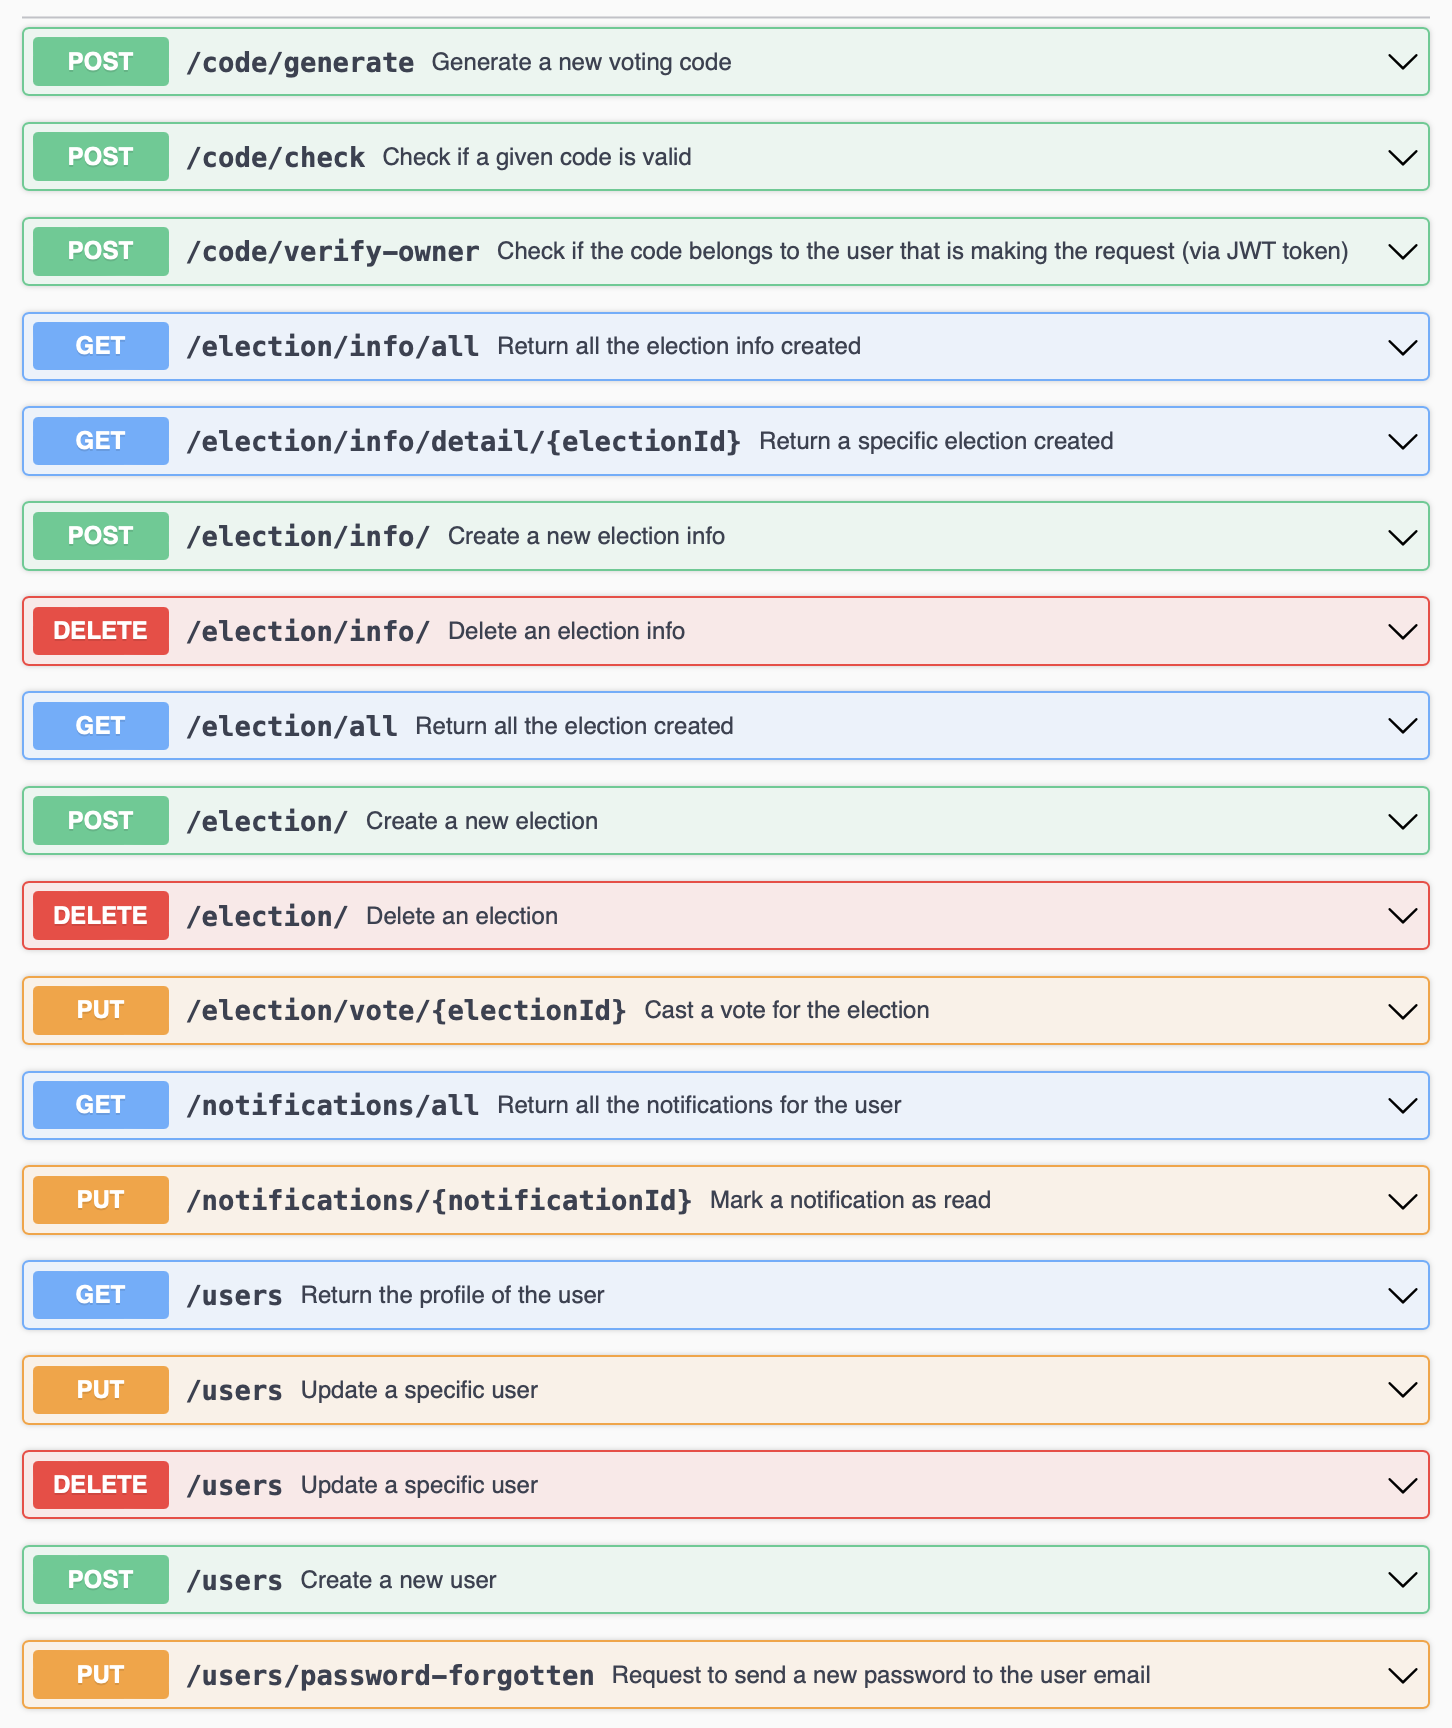
\includegraphics[width=\textwidth]{./figures/backend-routes/api.png}
    \caption{API routes.}
    \label{fig:backend-routes-api}
\end{figure}

\begin{figure}
    \centering
    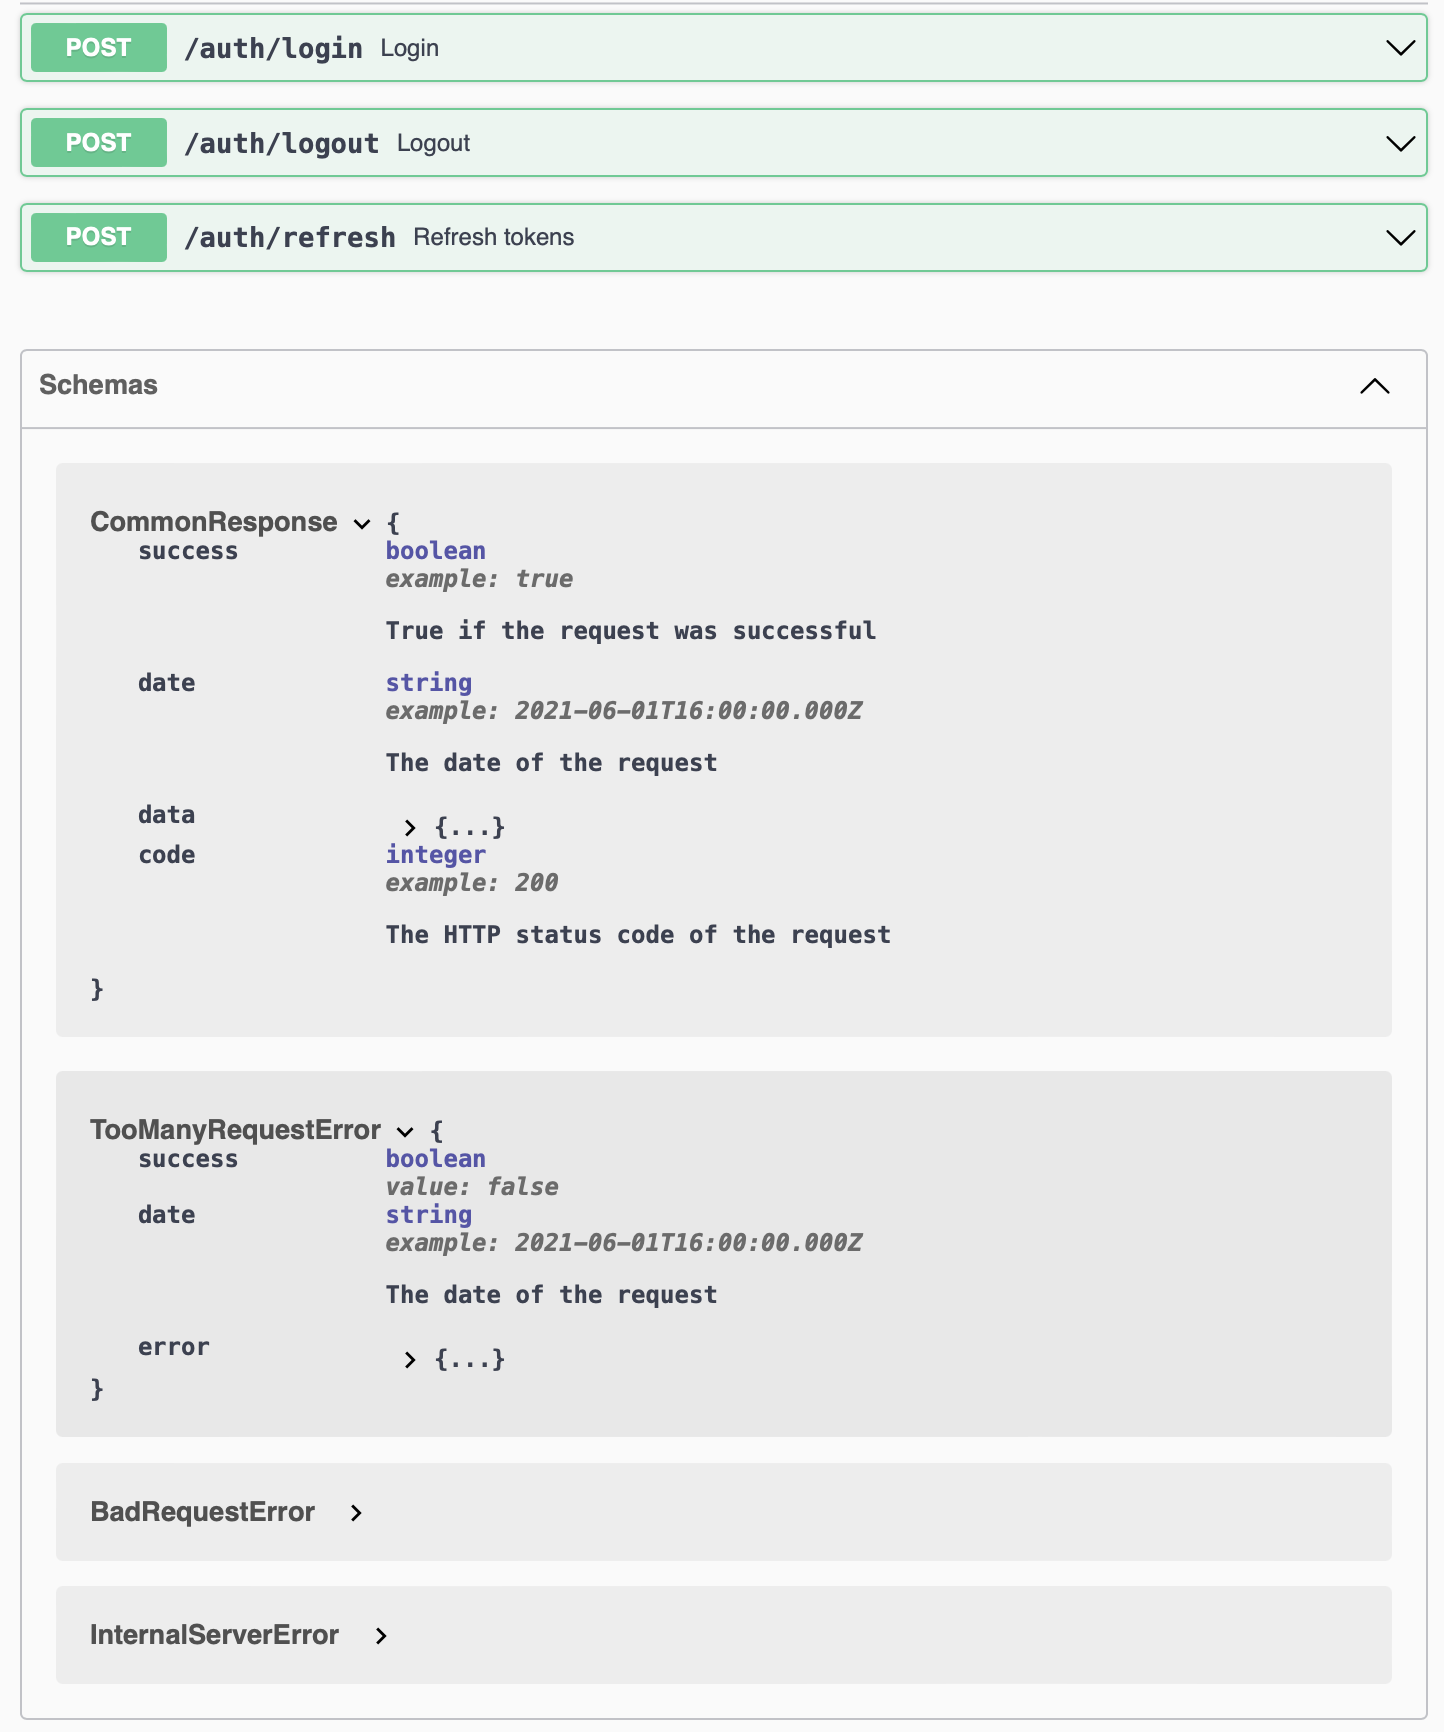
\includegraphics[width=\textwidth]{./figures/backend-routes/auth.png}
    \caption{Auth service routes, along with the schema of the response.}
    \label{fig:backend-routes-auth}
\end{figure}

\subsubsection{Real time updates and notifications with \texttt{Socket.io}}

As mentioned in \Cref{sec:technologies}, \texttt{Socket.io} have been used for the implementation of real-time updates and notifications.

More in details, the kind of updates that are interesting from the client perspective and to be updated reactively without the need of refreshing the page are the following:

\begin{itemize}
    \item when someone cast a vote the details page must be updated to reflect the new turnout of the election;
    \item when an election opens or closes the details page and the dashboard must be updated to reflect the new status of the election and display the results if it is closed;
\end{itemize}

Moreover, whenever an important event occurs, the server must push to clients a notification to inform them about it.
%
Following a comprehensive requirements analysis, the following events have emerged as crucial and indispensable for the successful implementation of our project:

\begin{itemize}
    \item when a new election is created;
    \item when an election is about to close.
\end{itemize}


Concerning the notifications they are emitted in broadcast to all connected clients, which in turns register the callback to execute whenever a new event is received.

\jsimport[
    caption={},
    label={lst:notifications}
]{listings/emitTurnout.ts}

For the elections updates we leverage the \texttt{Socket.io} rooms mechanism: a room is created for each election and the clients that are interested in receiving updates for a specific election will join the room associated with it.

\begin{figure}
    \centering
    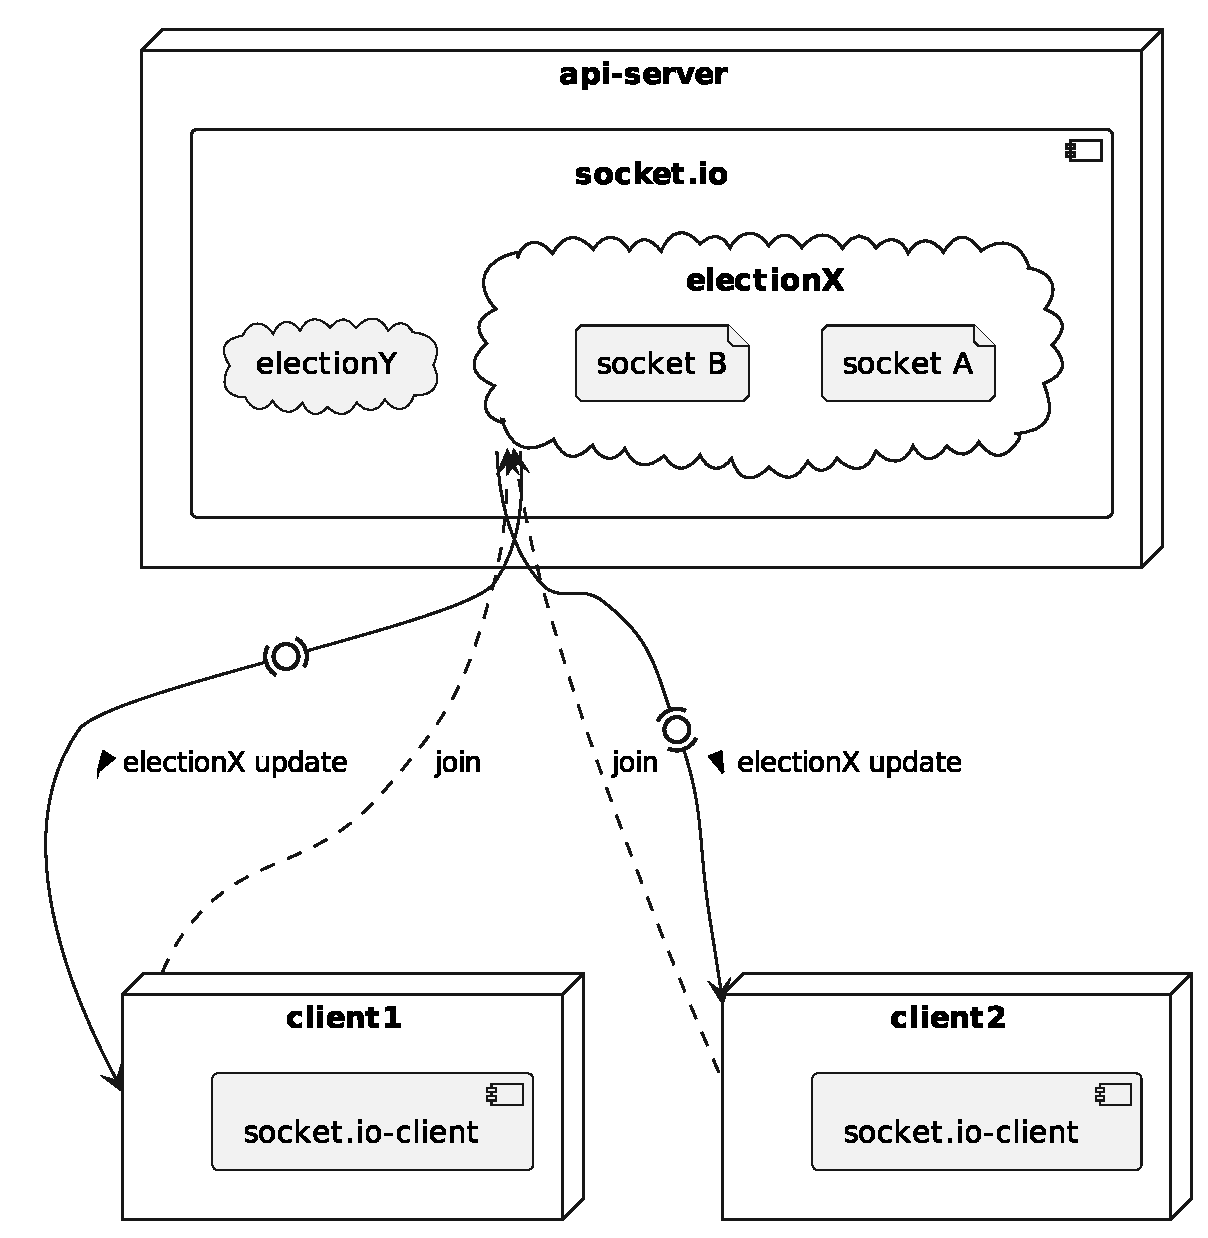
\includegraphics[width=0.7\linewidth]{figures/socket-io-rooms.eps}
    \caption{\texttt{Socket.io} rooms mechanism used to notify clients about election updates.}
    \label{fig:socket-io-rooms} 
\end{figure}

Also, since elections can be, and generally are, created to open at some time in the future, it must be possible, on the part of the server, to schedule them. 
%
This is achieved by registering a callback that is scheduled to be executed at the time the notification is to be triggered. 
%
An abnormal restart of the server, however, would erase all schedules, preventing clients from being notified. 
%
To overcome this problem, the scheduled notifications are stored within MongoDB so that at any server restart, it may be possible to reschedule notifications that have not yet been delivered.

\jsimport[
    caption={},
    label={lst:notifications}
]{listings/notifications.ts}


\subsection{Frontend}

\subsubsection{Stores}

We've collected all backend APIs in stores, one for each main entity of the system, which also hold information required in communications.

\subsubsection{Vue Components}

Given the reusable and modular nature offered by Vue's component, we've implemented several components to manage custom content and logic.
By means of custom emit events and props, the nested structure offered by components can be crossed from parent to child components bidirectionally, triggering events in child components that propagate up to the parents.

\section{Story board}

The homepage of the system is shown in \Cref{fig:homepage}.

A system administrator can authenticate into the system by entering his credentials (\Cref{fig:login-admin}) and is automatically redirected to the dashboard.

Through the navigation bar the administrator is able to create a new election entering the goal of the election, opening and closing date and time, number of participants and choices (white ballot is always added to those entered by the user) (\Cref{fig:creation-election}).

\newgeometry{margin=1.0cm}
\begin{figure}
    \centering
    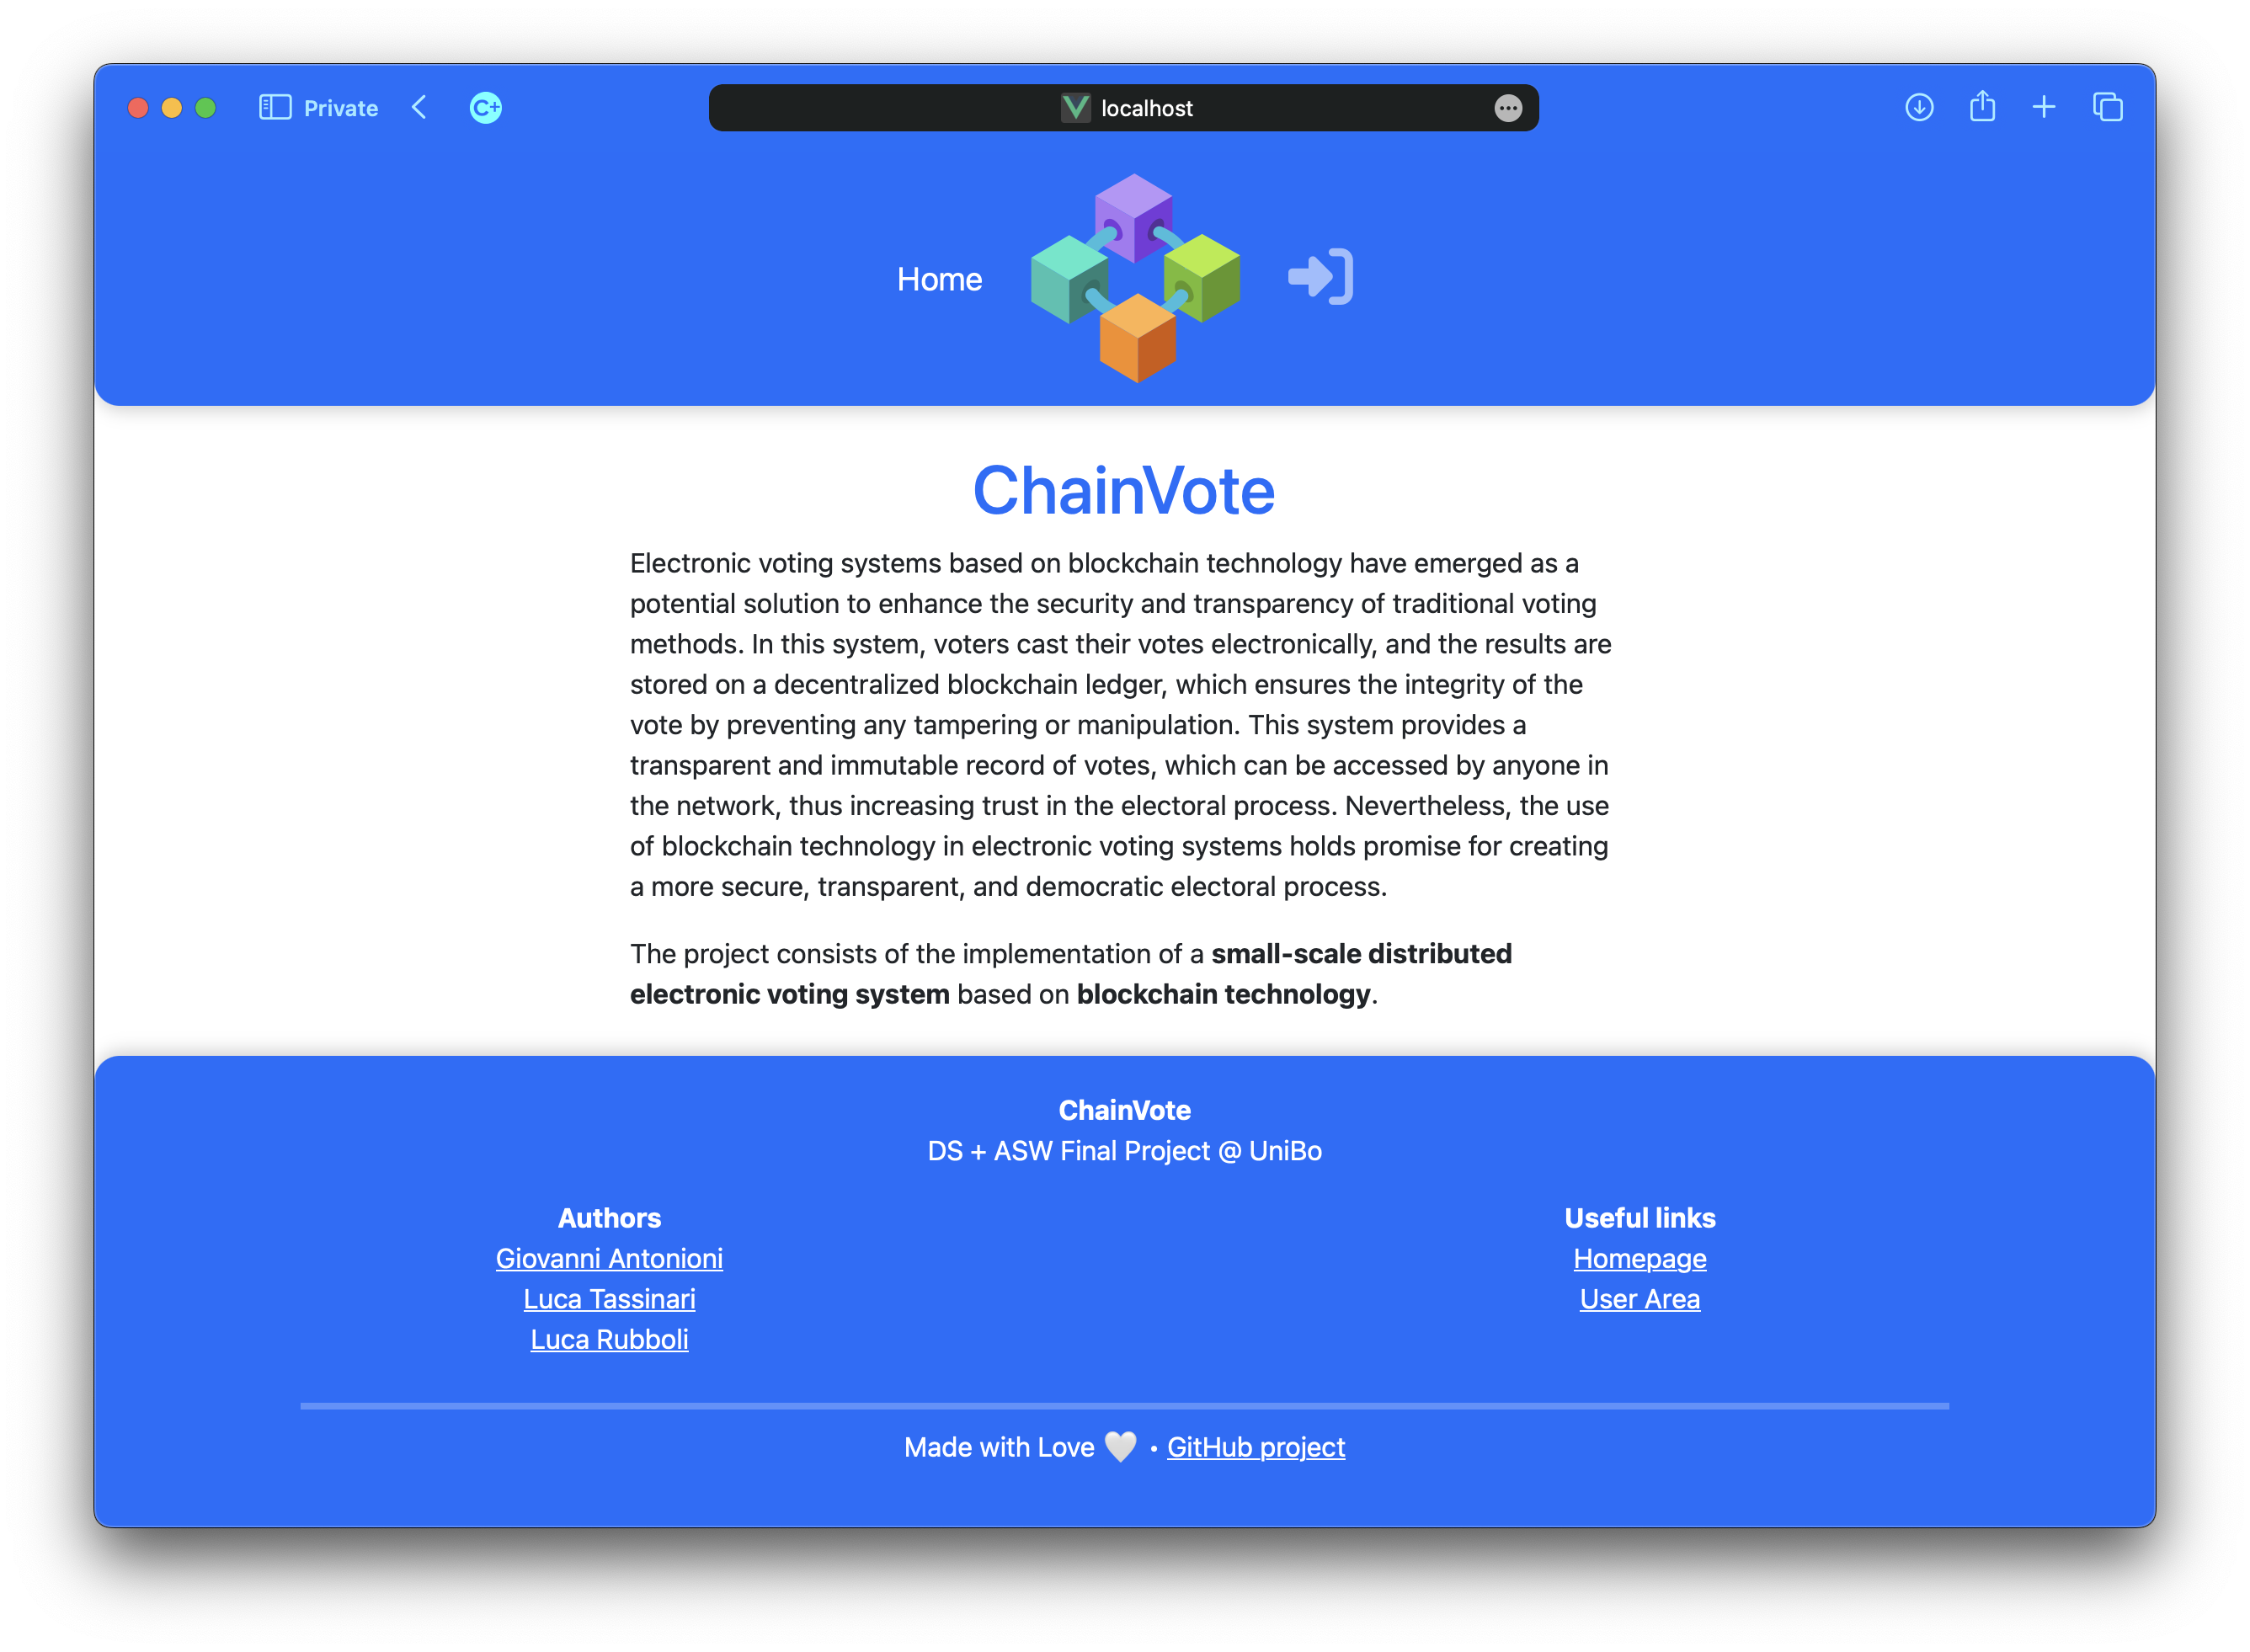
\includegraphics[width=0.9\linewidth]{figures/story-board/1-index.png}
    \caption{Homepage of the web app.}
    \label{fig:homepage}
\end{figure}

\begin{figure}
    \centering
    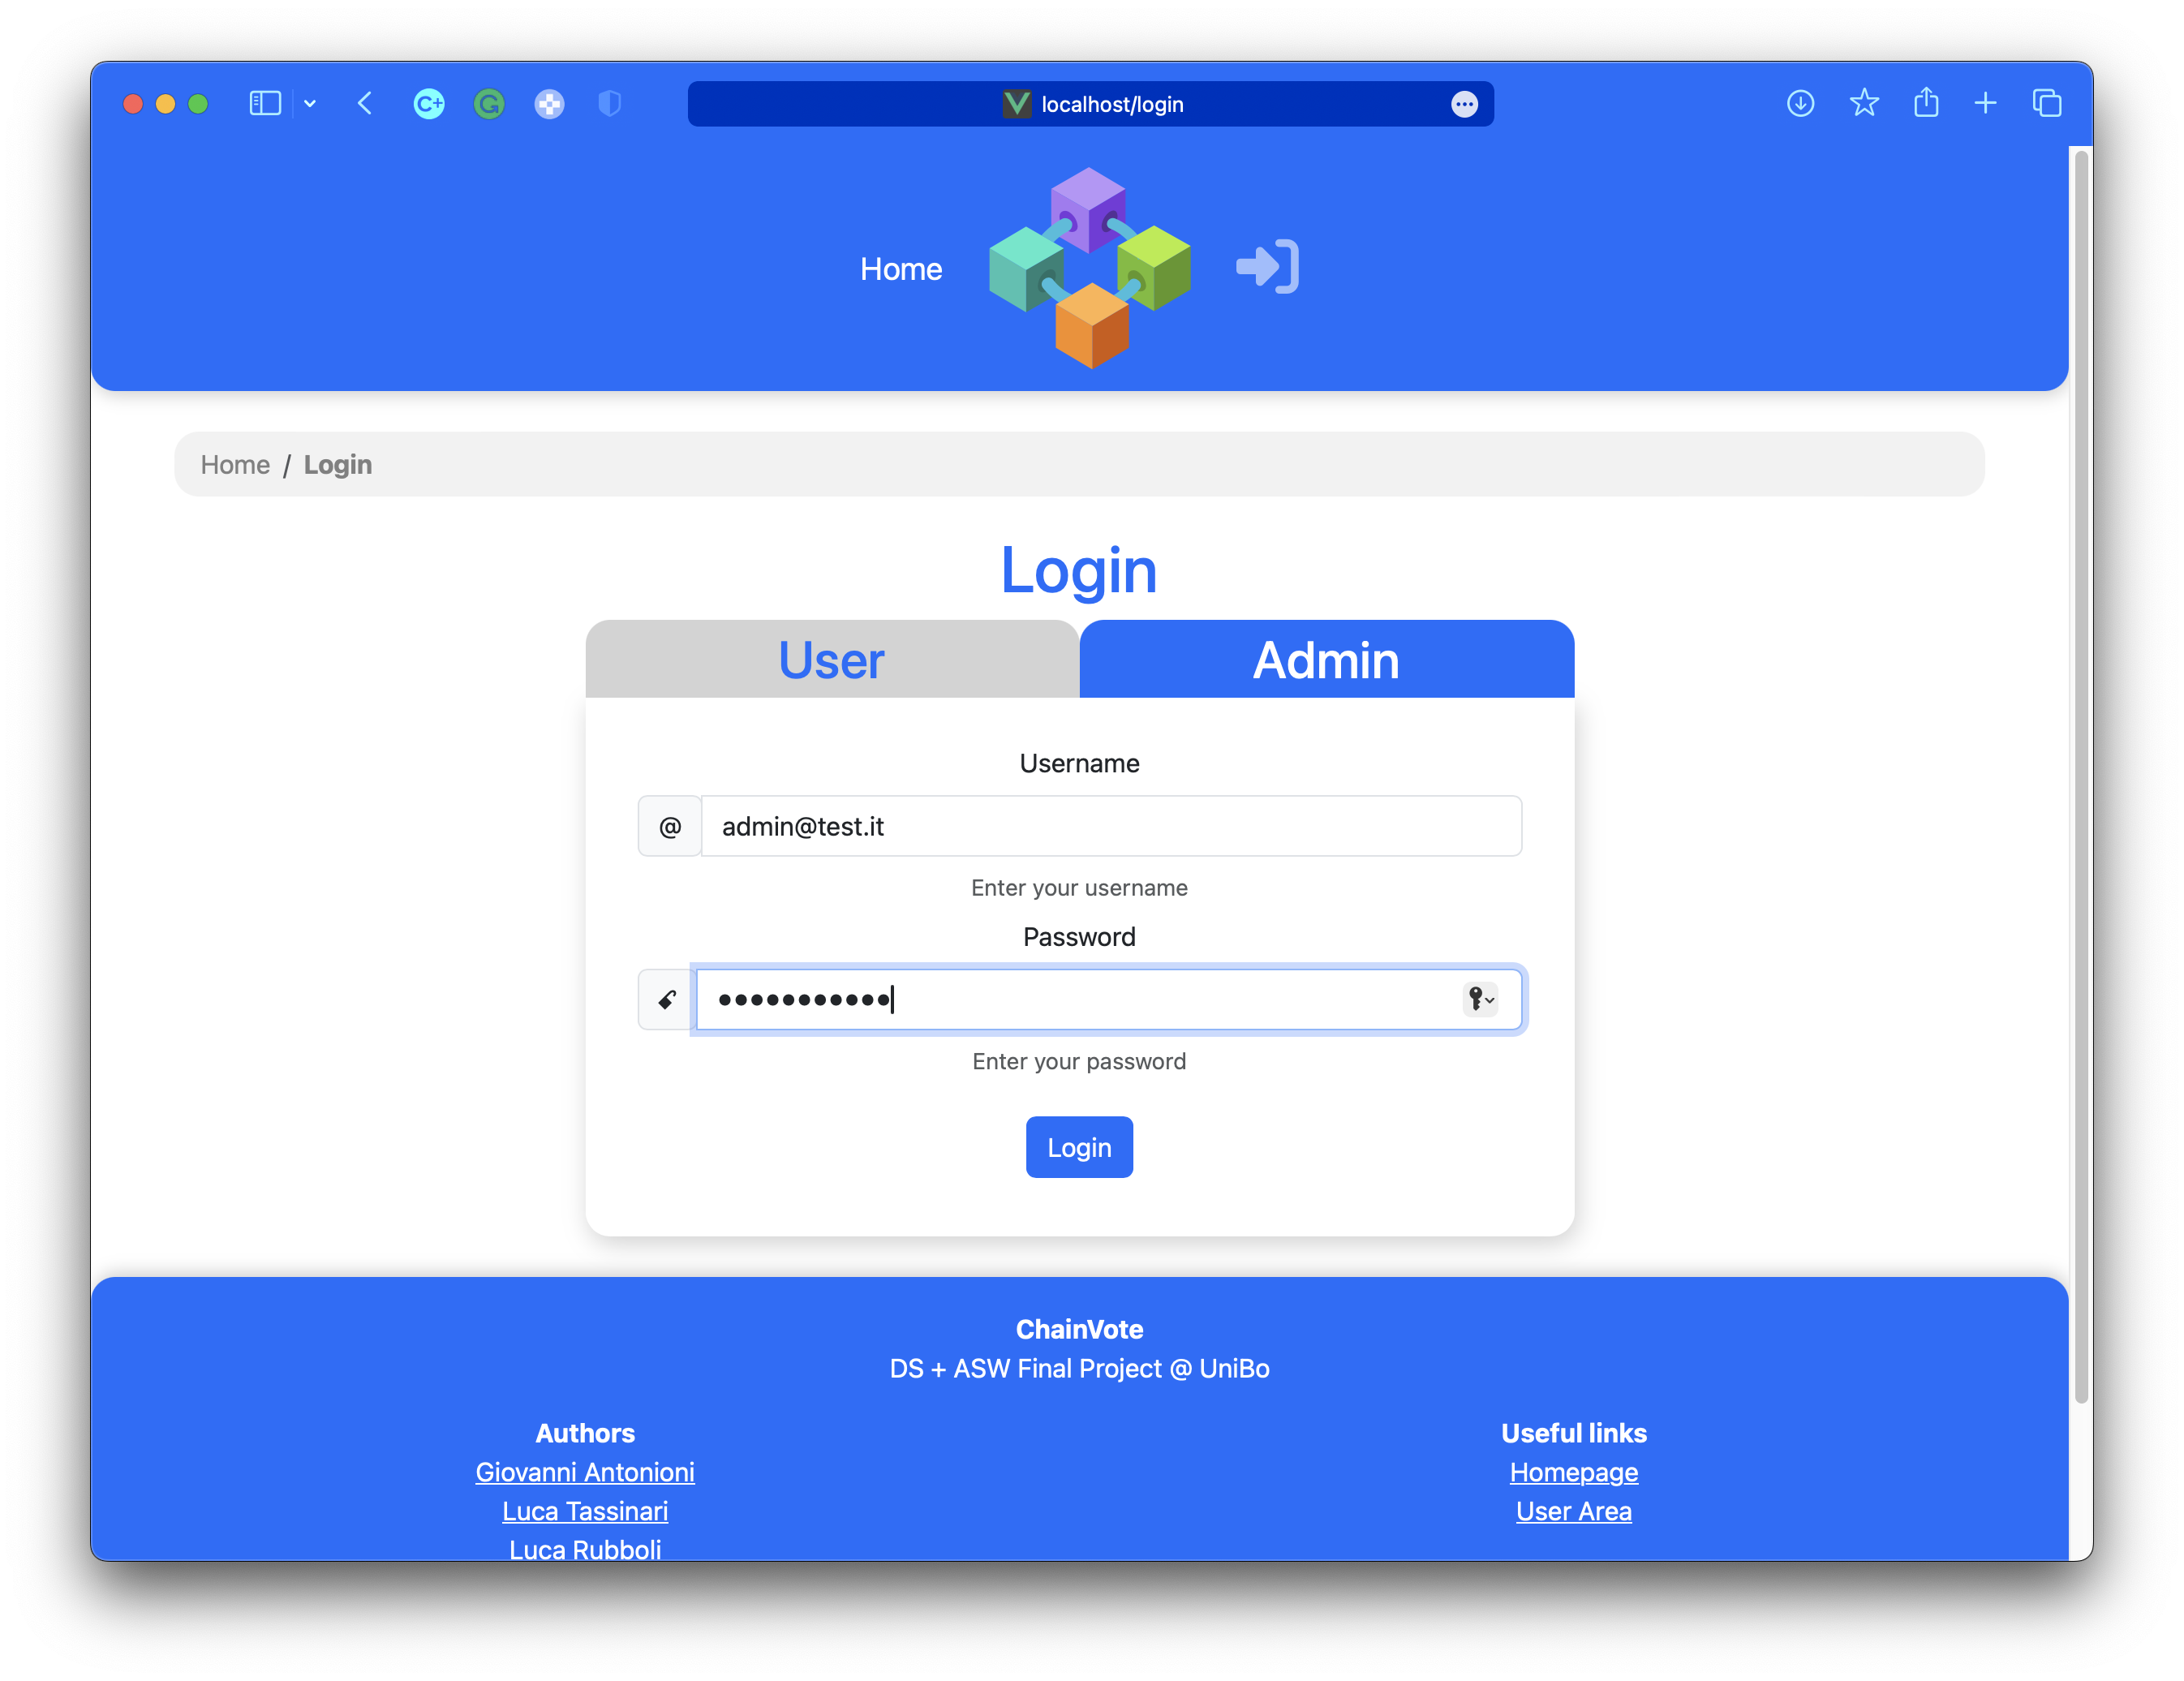
\includegraphics[width=0.9\linewidth]{figures/story-board/2-login-admin.png}
    \caption{Login of the administrator view.}
    \label{fig:login-admin}
\end{figure}

\begin{figure}
    \centering
    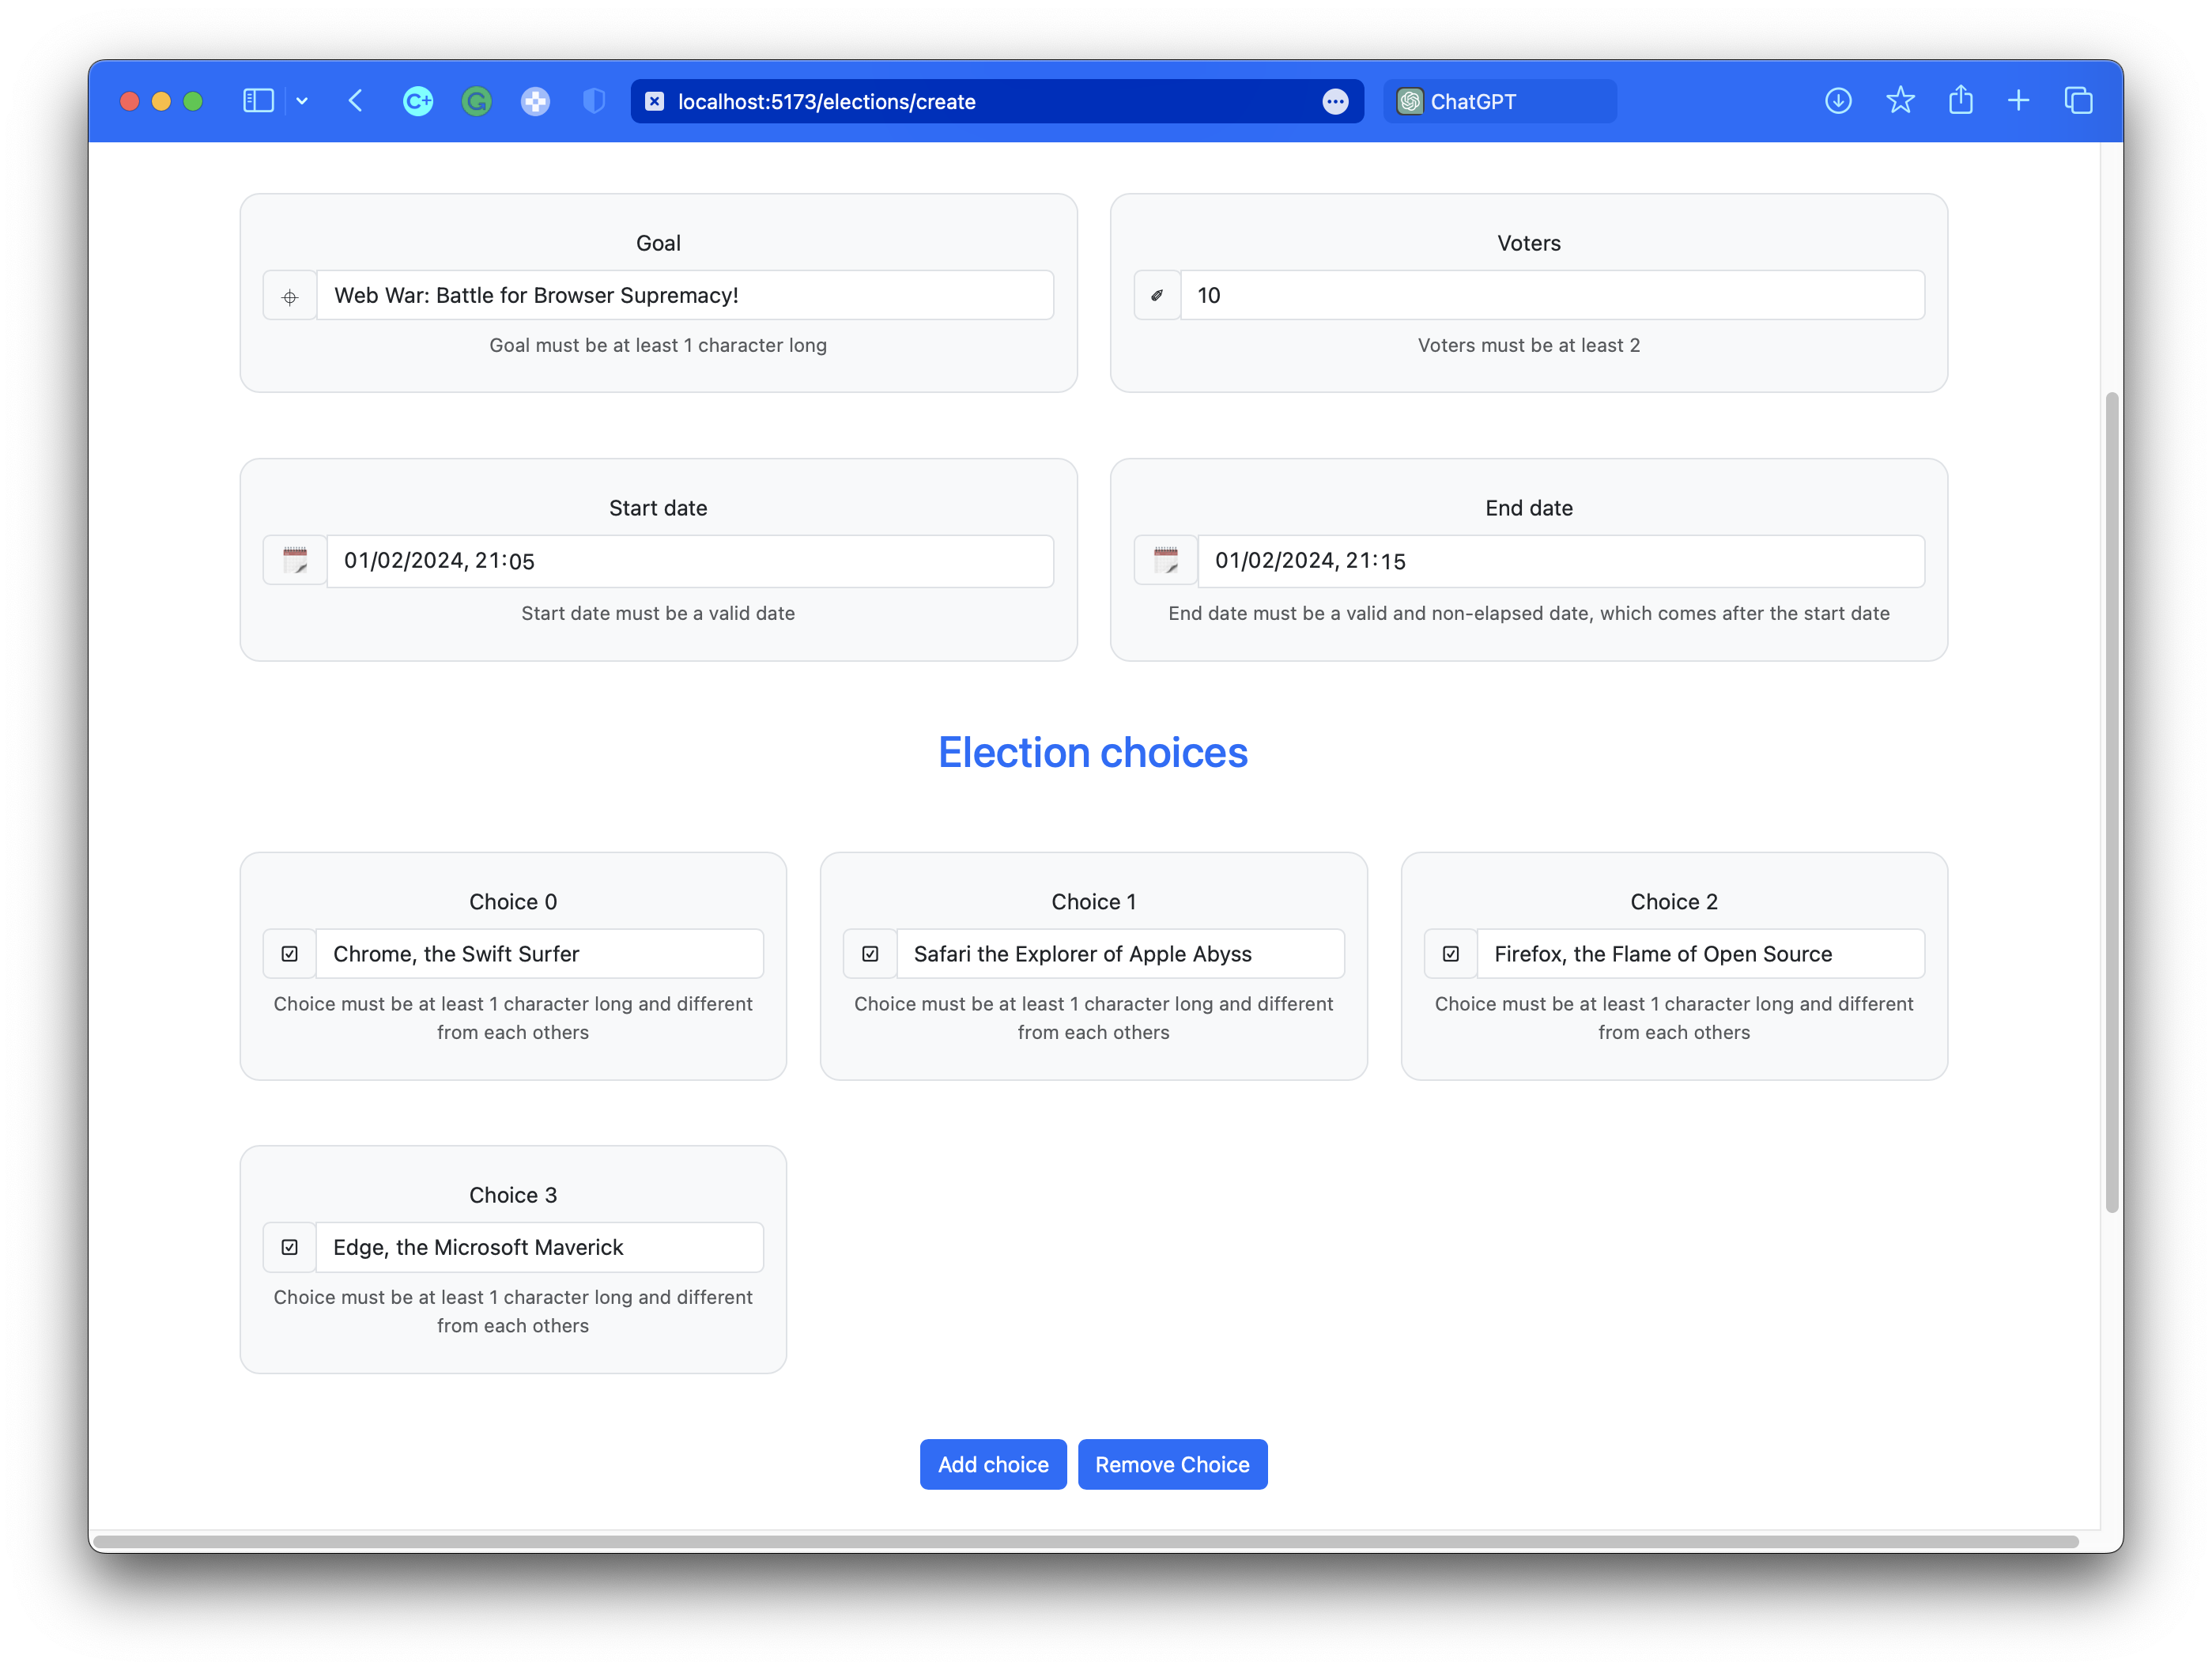
\includegraphics[width=0.88\linewidth]{figures/story-board/3-creation-election.png}
    \caption{Creation of a new election view.}
    \label{fig:creation-election}
\end{figure}

\begin{figure}
    \centering
    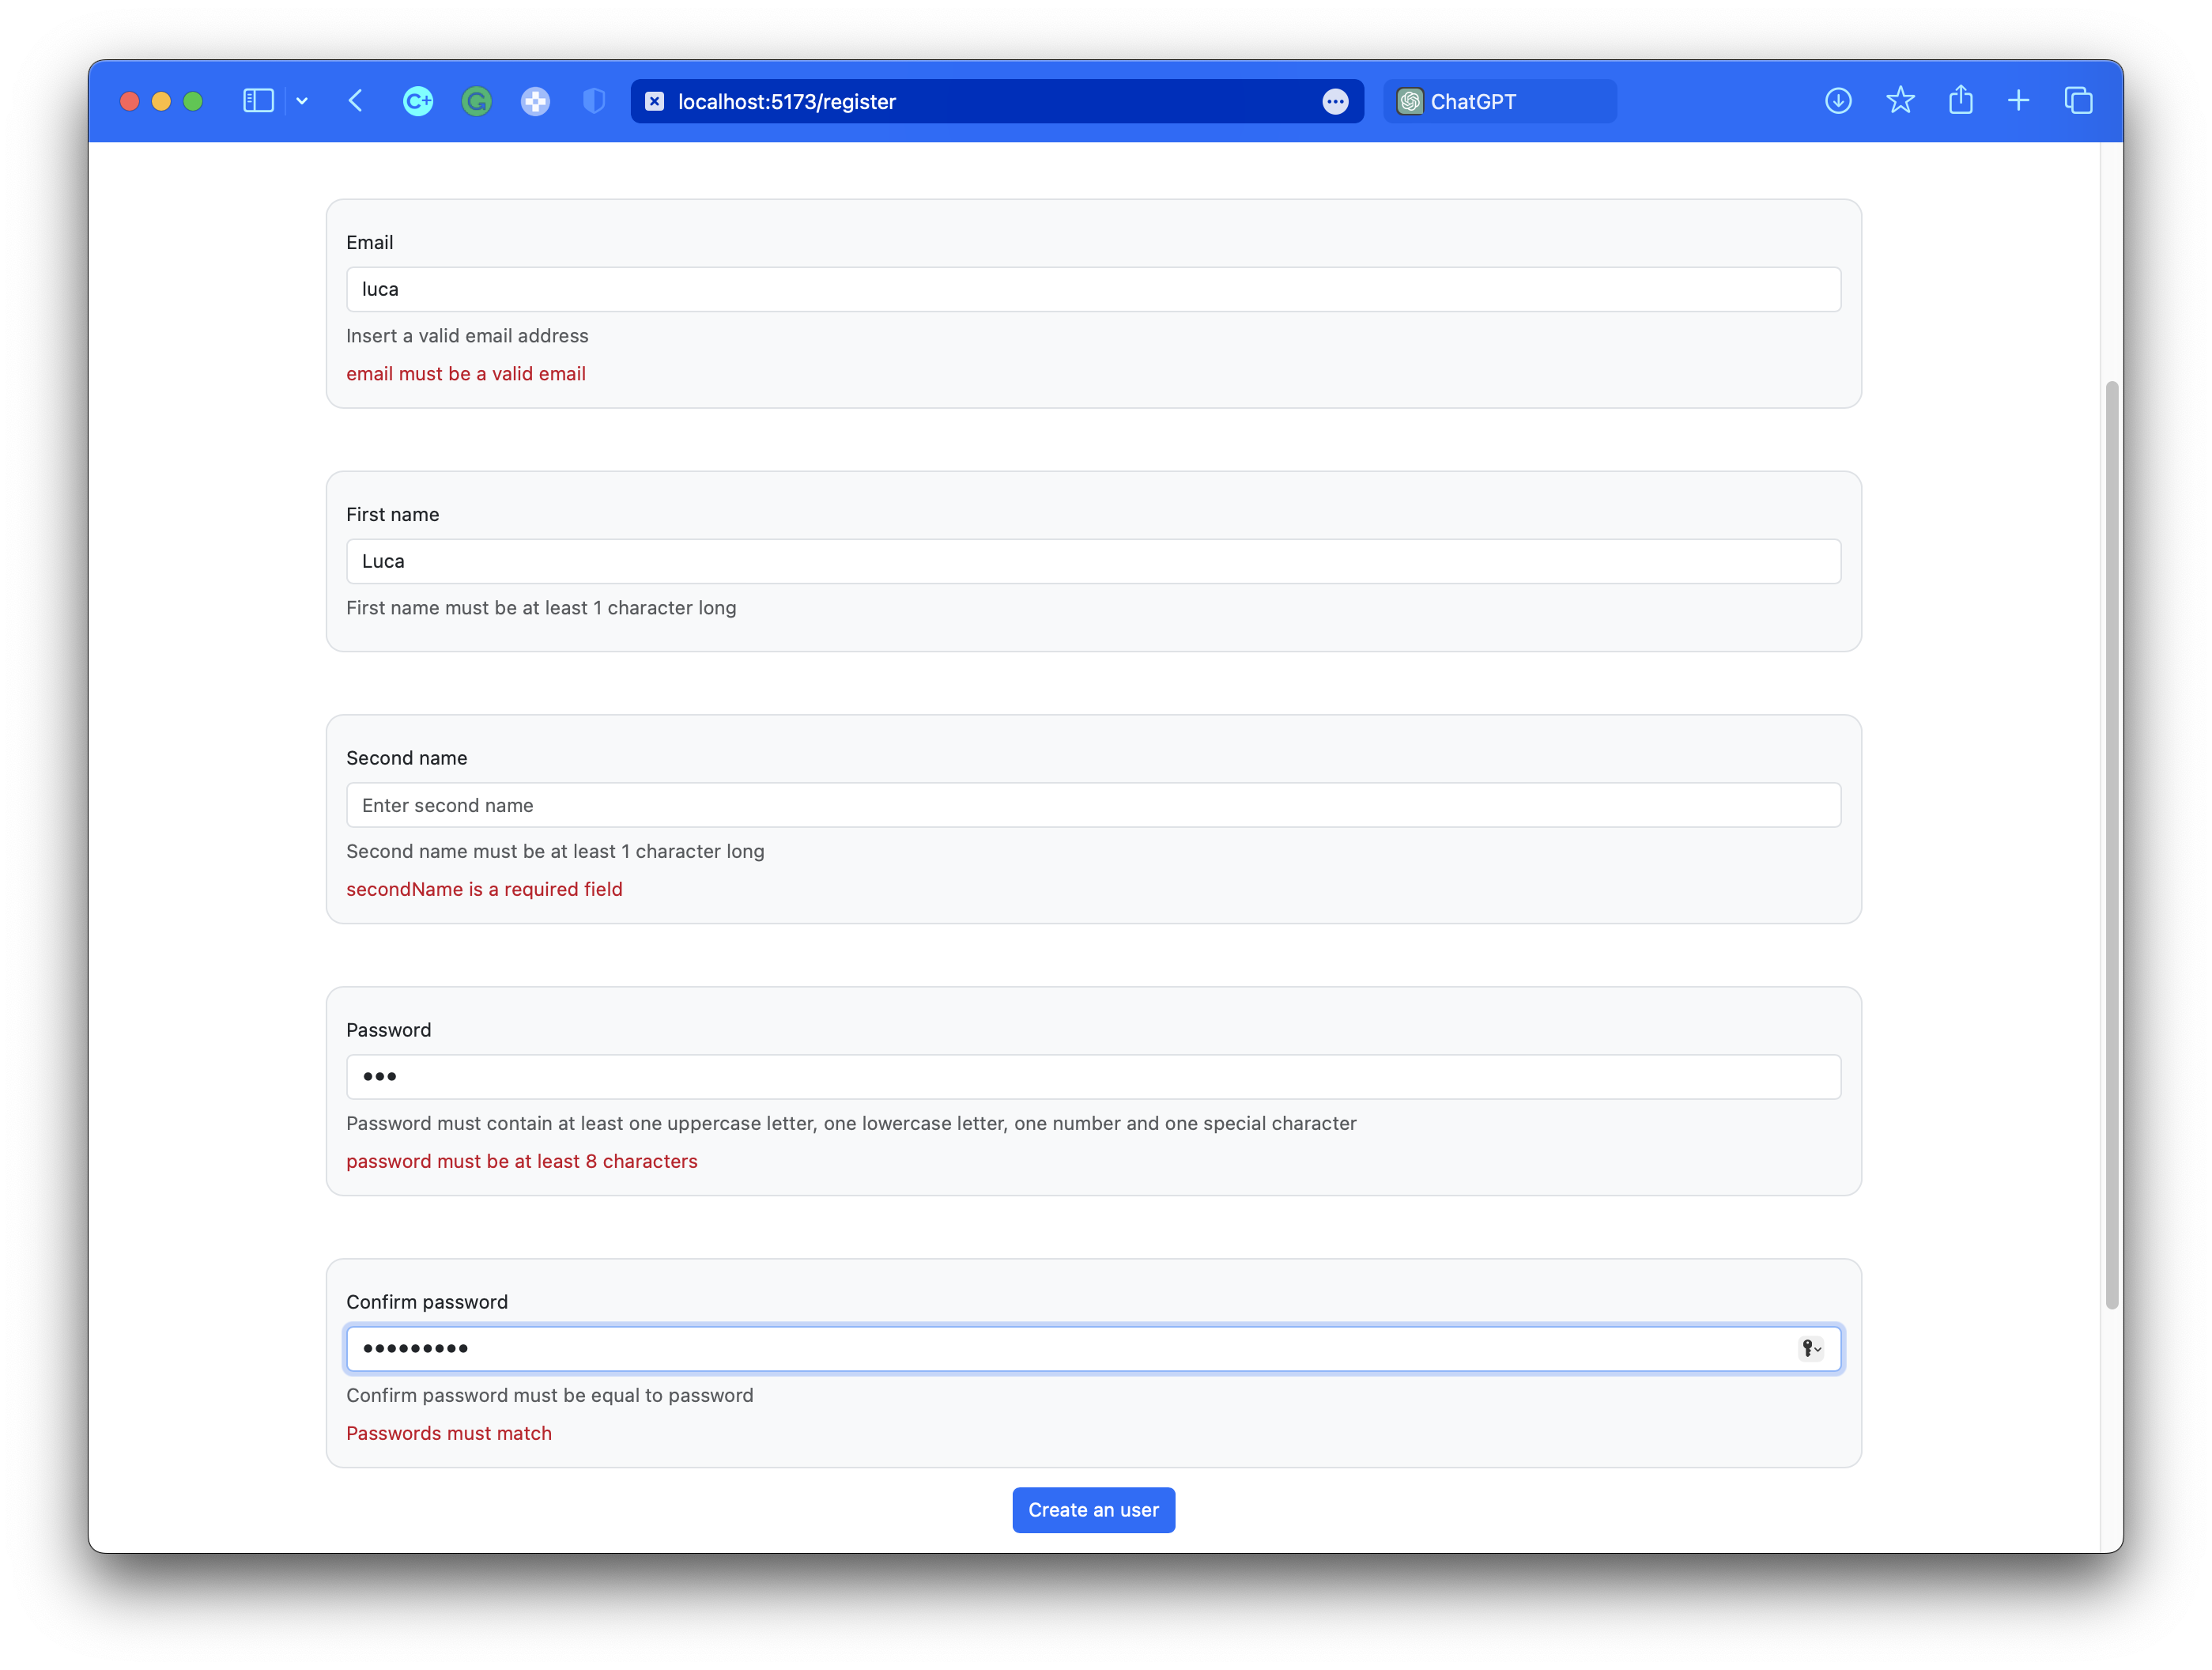
\includegraphics[width=0.88\linewidth]{figures/story-board/4-user-registration.png}
    \caption{User registration view. Non correct inputs are highlighted.}
    \label{fig:user-registration}
\end{figure}
\restoregeometry

A user can register into the system by entering its personal information (which are modifiable once logged in, \Cref{fig:user-area}), a valid email address and a password.
%
The inputs of the form (as every form of the website) are checked for correctness, displaying an error message if the given value is not valid (\Cref{fig:user-registration}).

Moreover, if the user forgets the password can request the generation of  new one which is sent to the email address provided during the registration (\Cref{fig:password-forgotten}).

After registration, the user can authenticate into the system by entering his or her credentials (\Cref{fig:user-login}) and is automatically directed to the dashboard where the most recent elections are displayed based on their status (open, closed, upcoming) (\Cref{fig:dashboard}).
%
For a more fluid experience, the user, clicking on the title of the election status, is redirected to the list where he or she can filter them in a more usable way (\Cref{fig:elections}).

\newgeometry{margin=1.0cm}
\begin{figure}
    \centering
    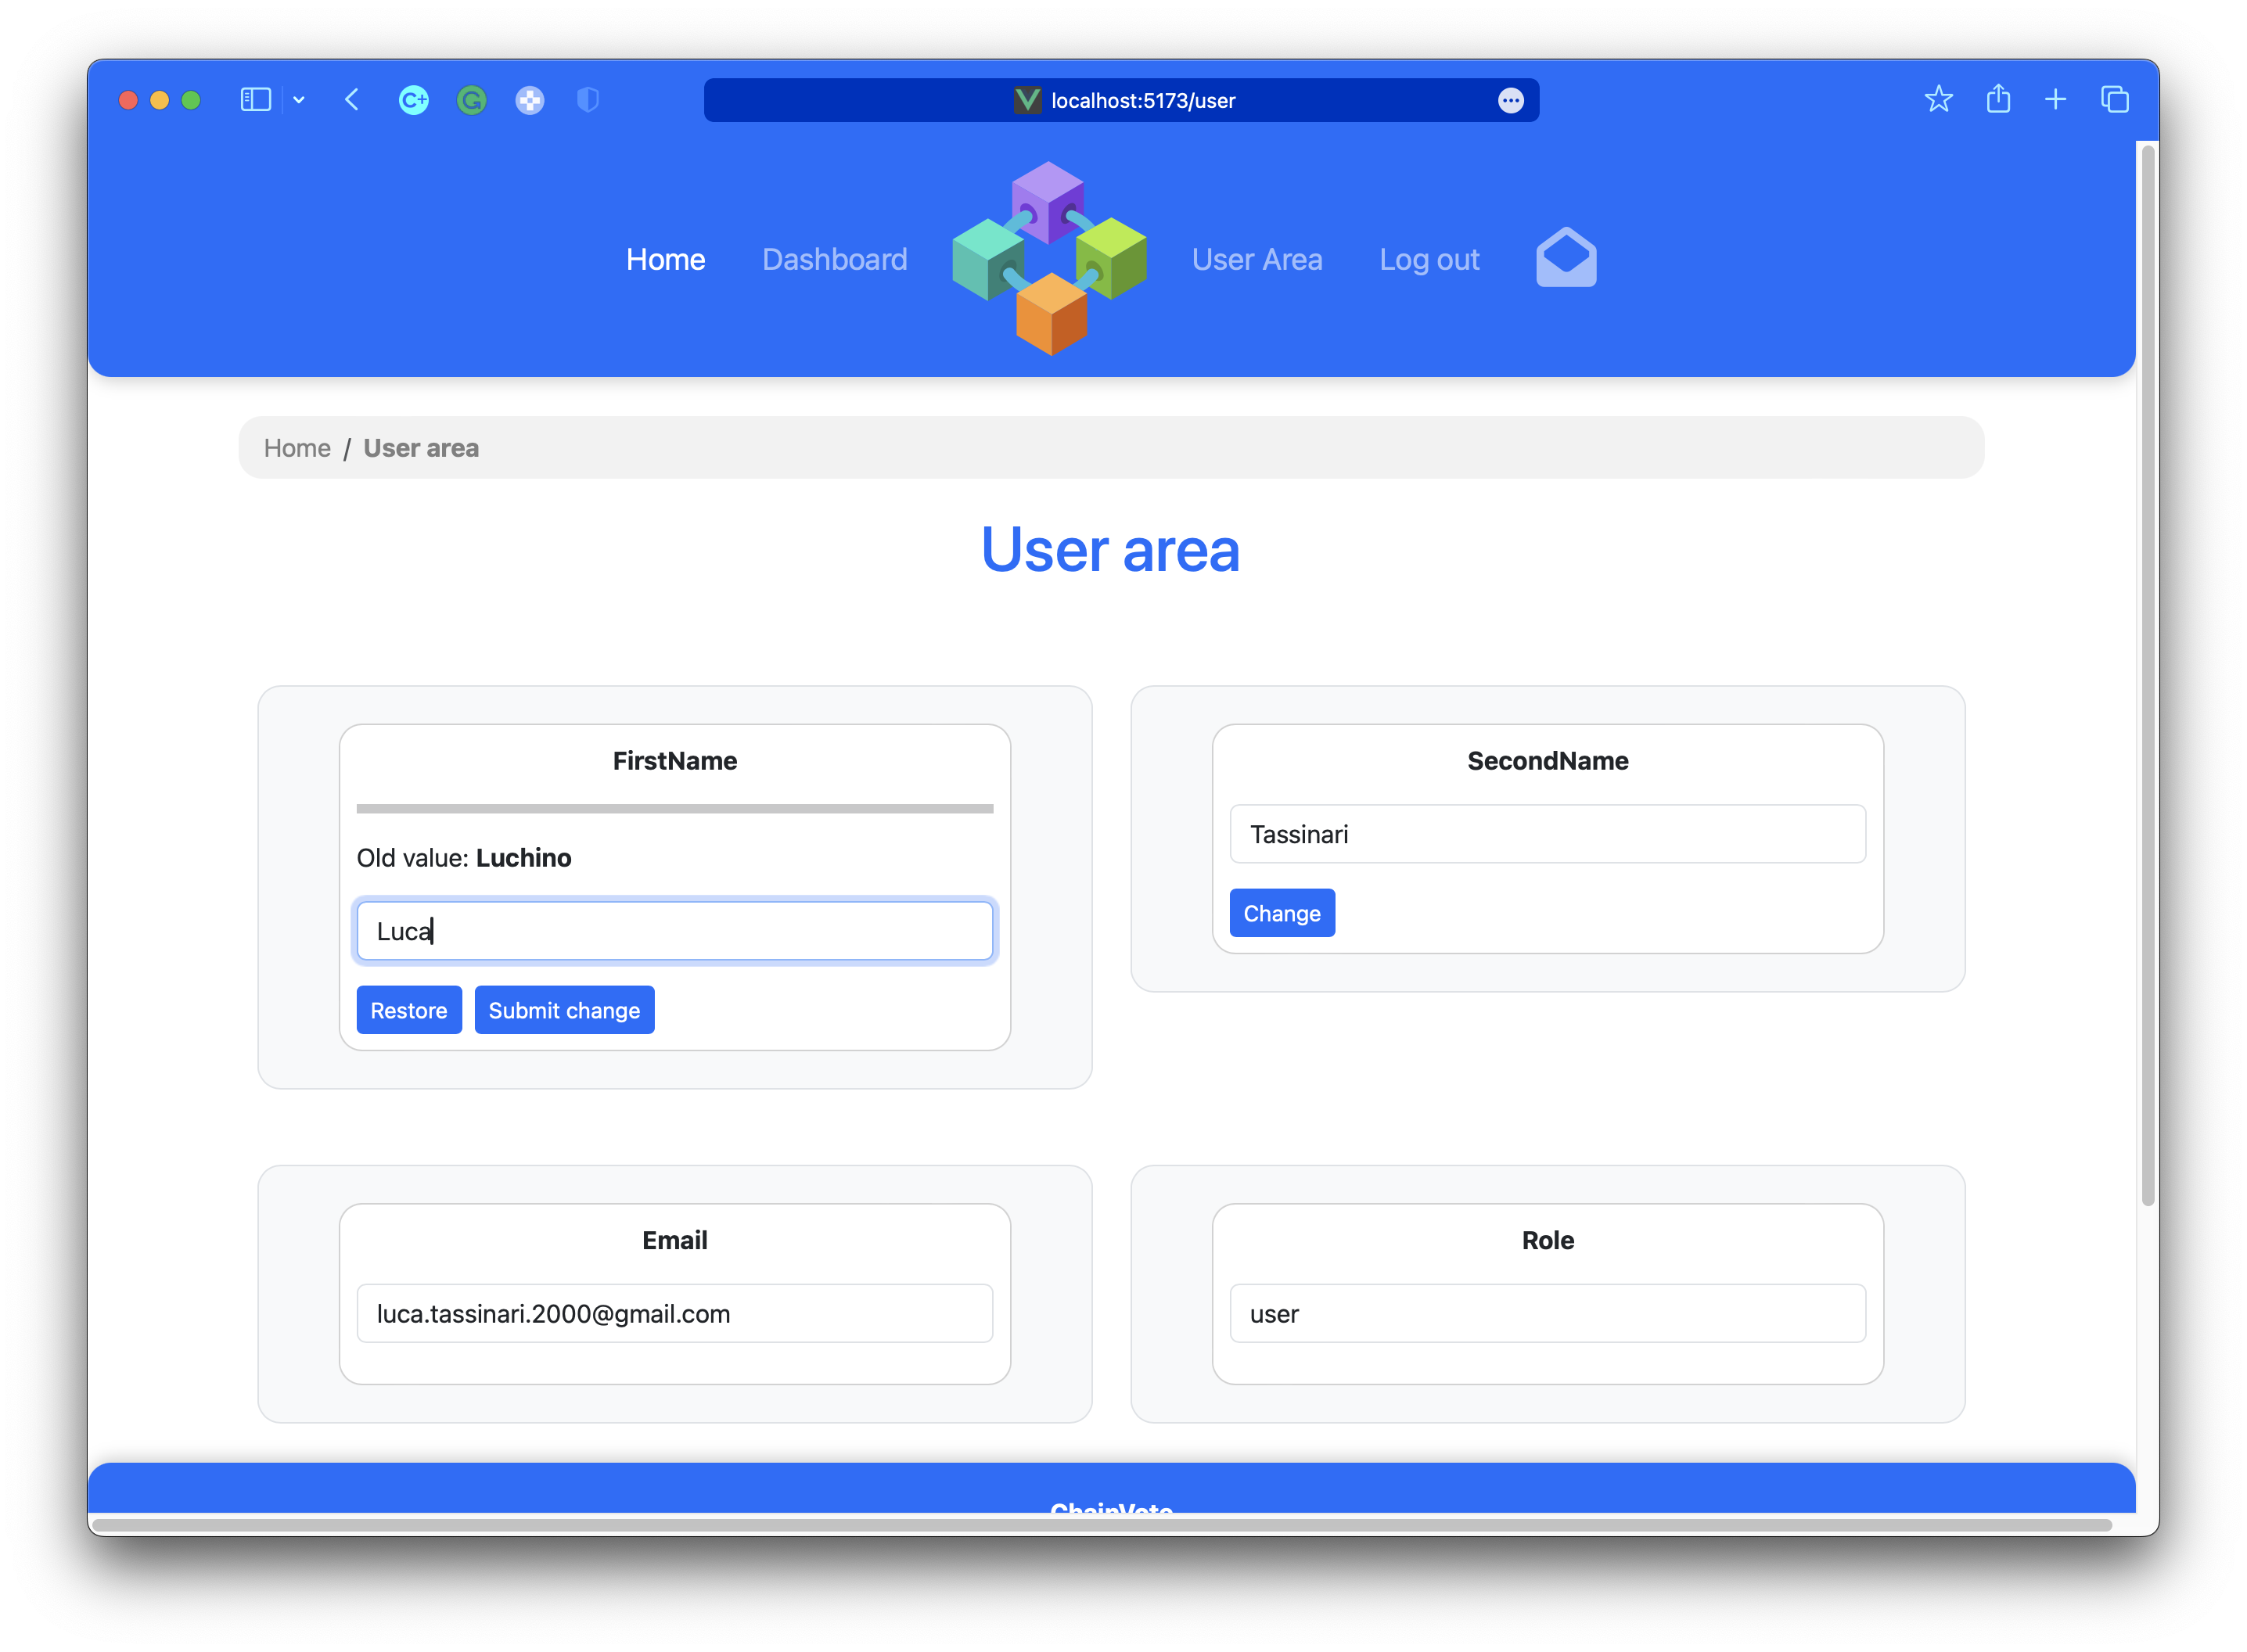
\includegraphics[width=0.9\linewidth]{figures/story-board/7-user-area.png}
    \label{fig:user-area}
    \caption{User area view.}
\end{figure}

\begin{figure}
    \centering
    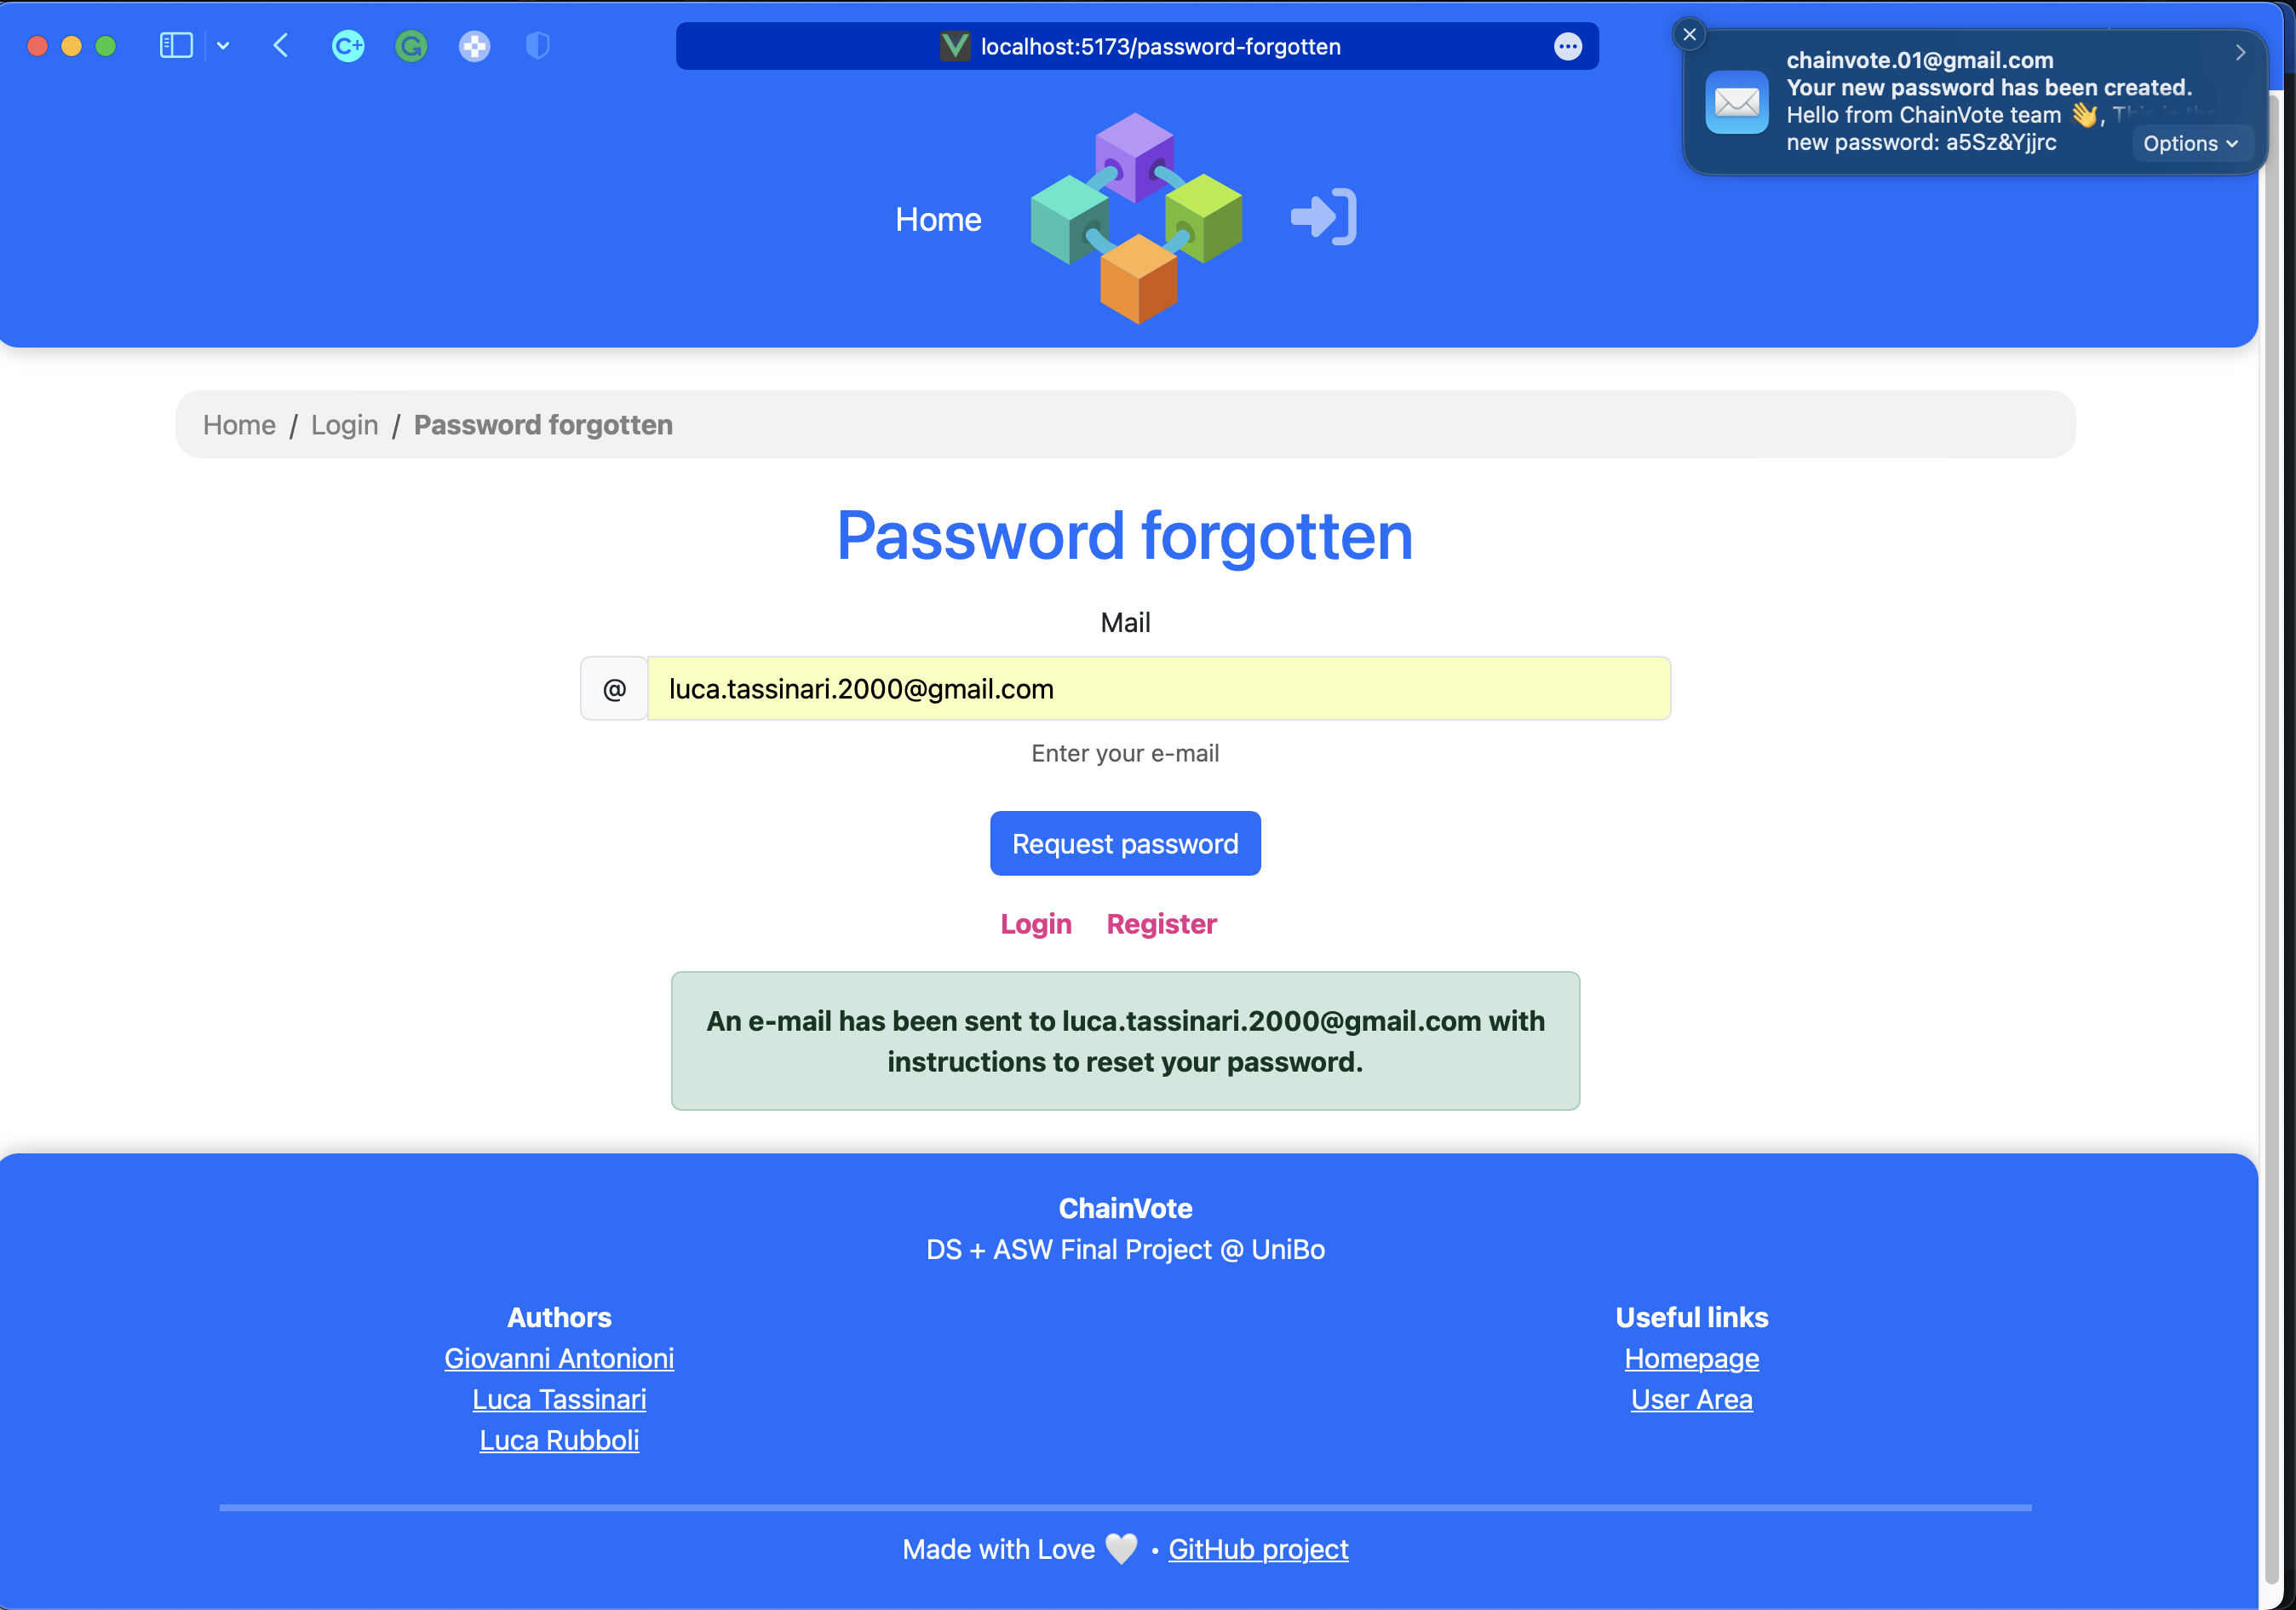
\includegraphics[width=0.8\linewidth]{figures/story-board/16-password-forgotten.png}
    \caption{Password forgotten view.}
    \label{fig:password-forgotten}
\end{figure}

\begin{figure}
    \centering
    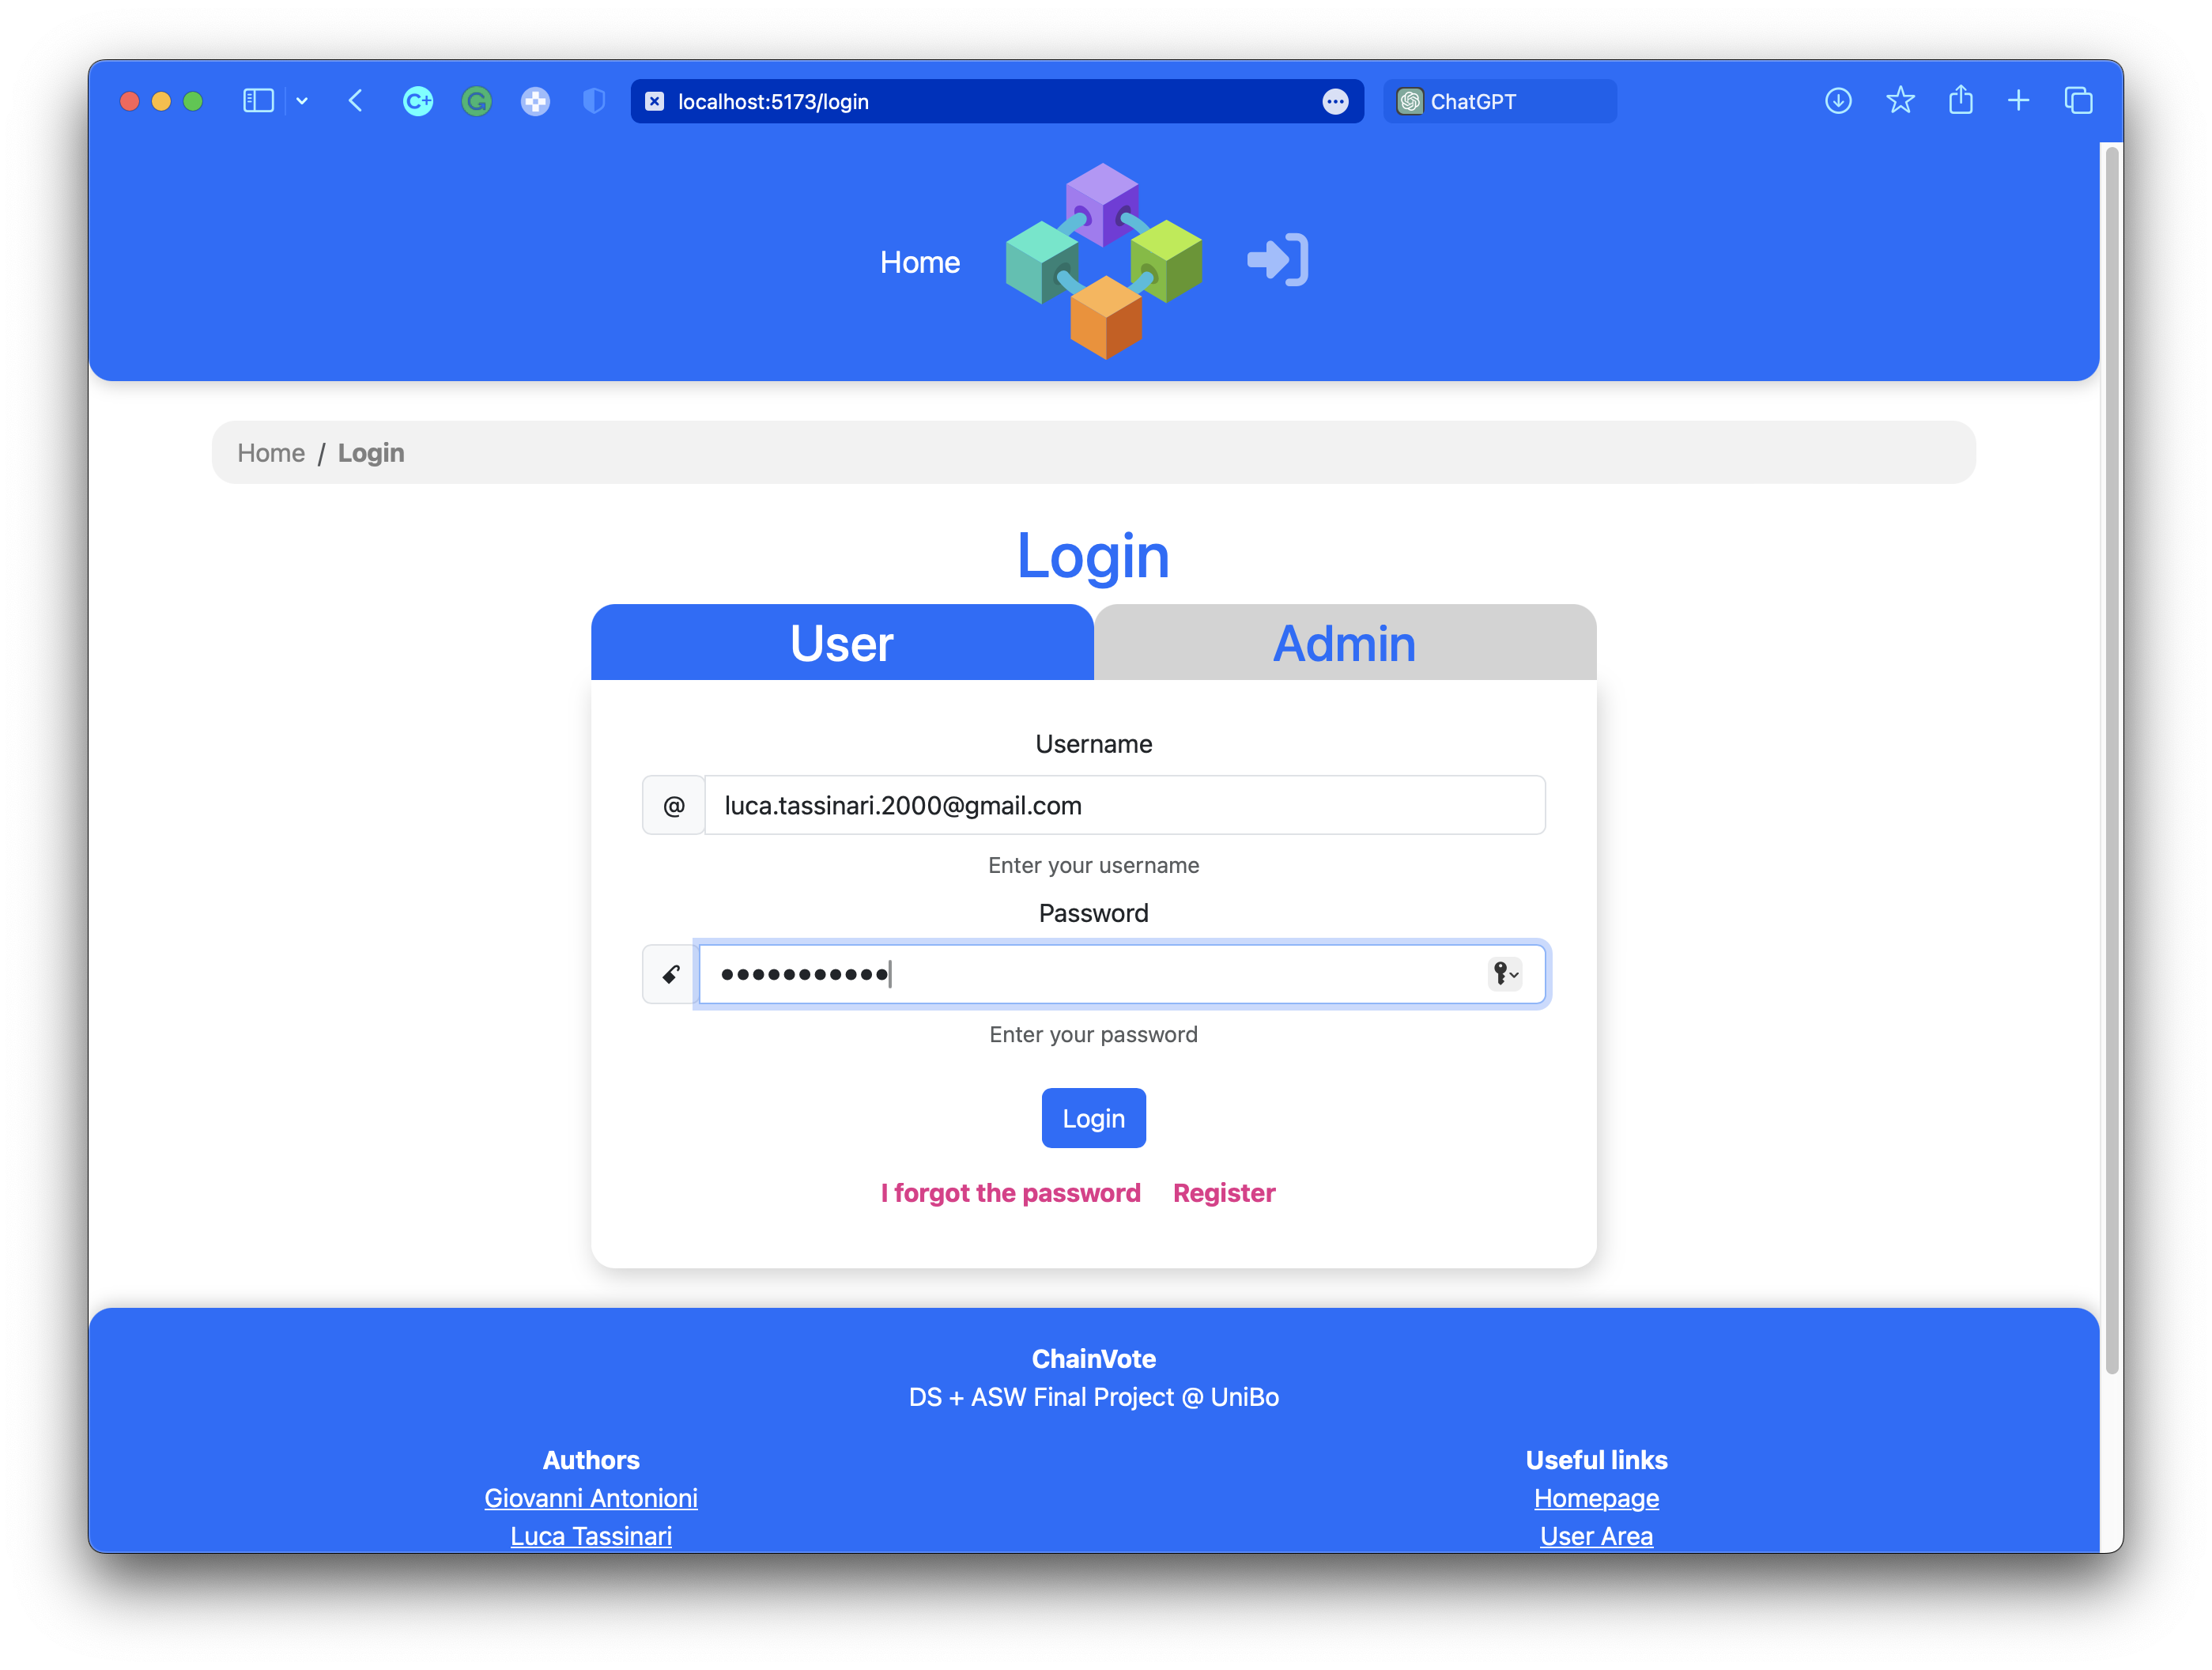
\includegraphics[width=0.9\linewidth]{figures/story-board/5-user-login.png}
    \caption{User login view.}
    \label{fig:user-login}
\end{figure}

\begin{figure}
    \centering
    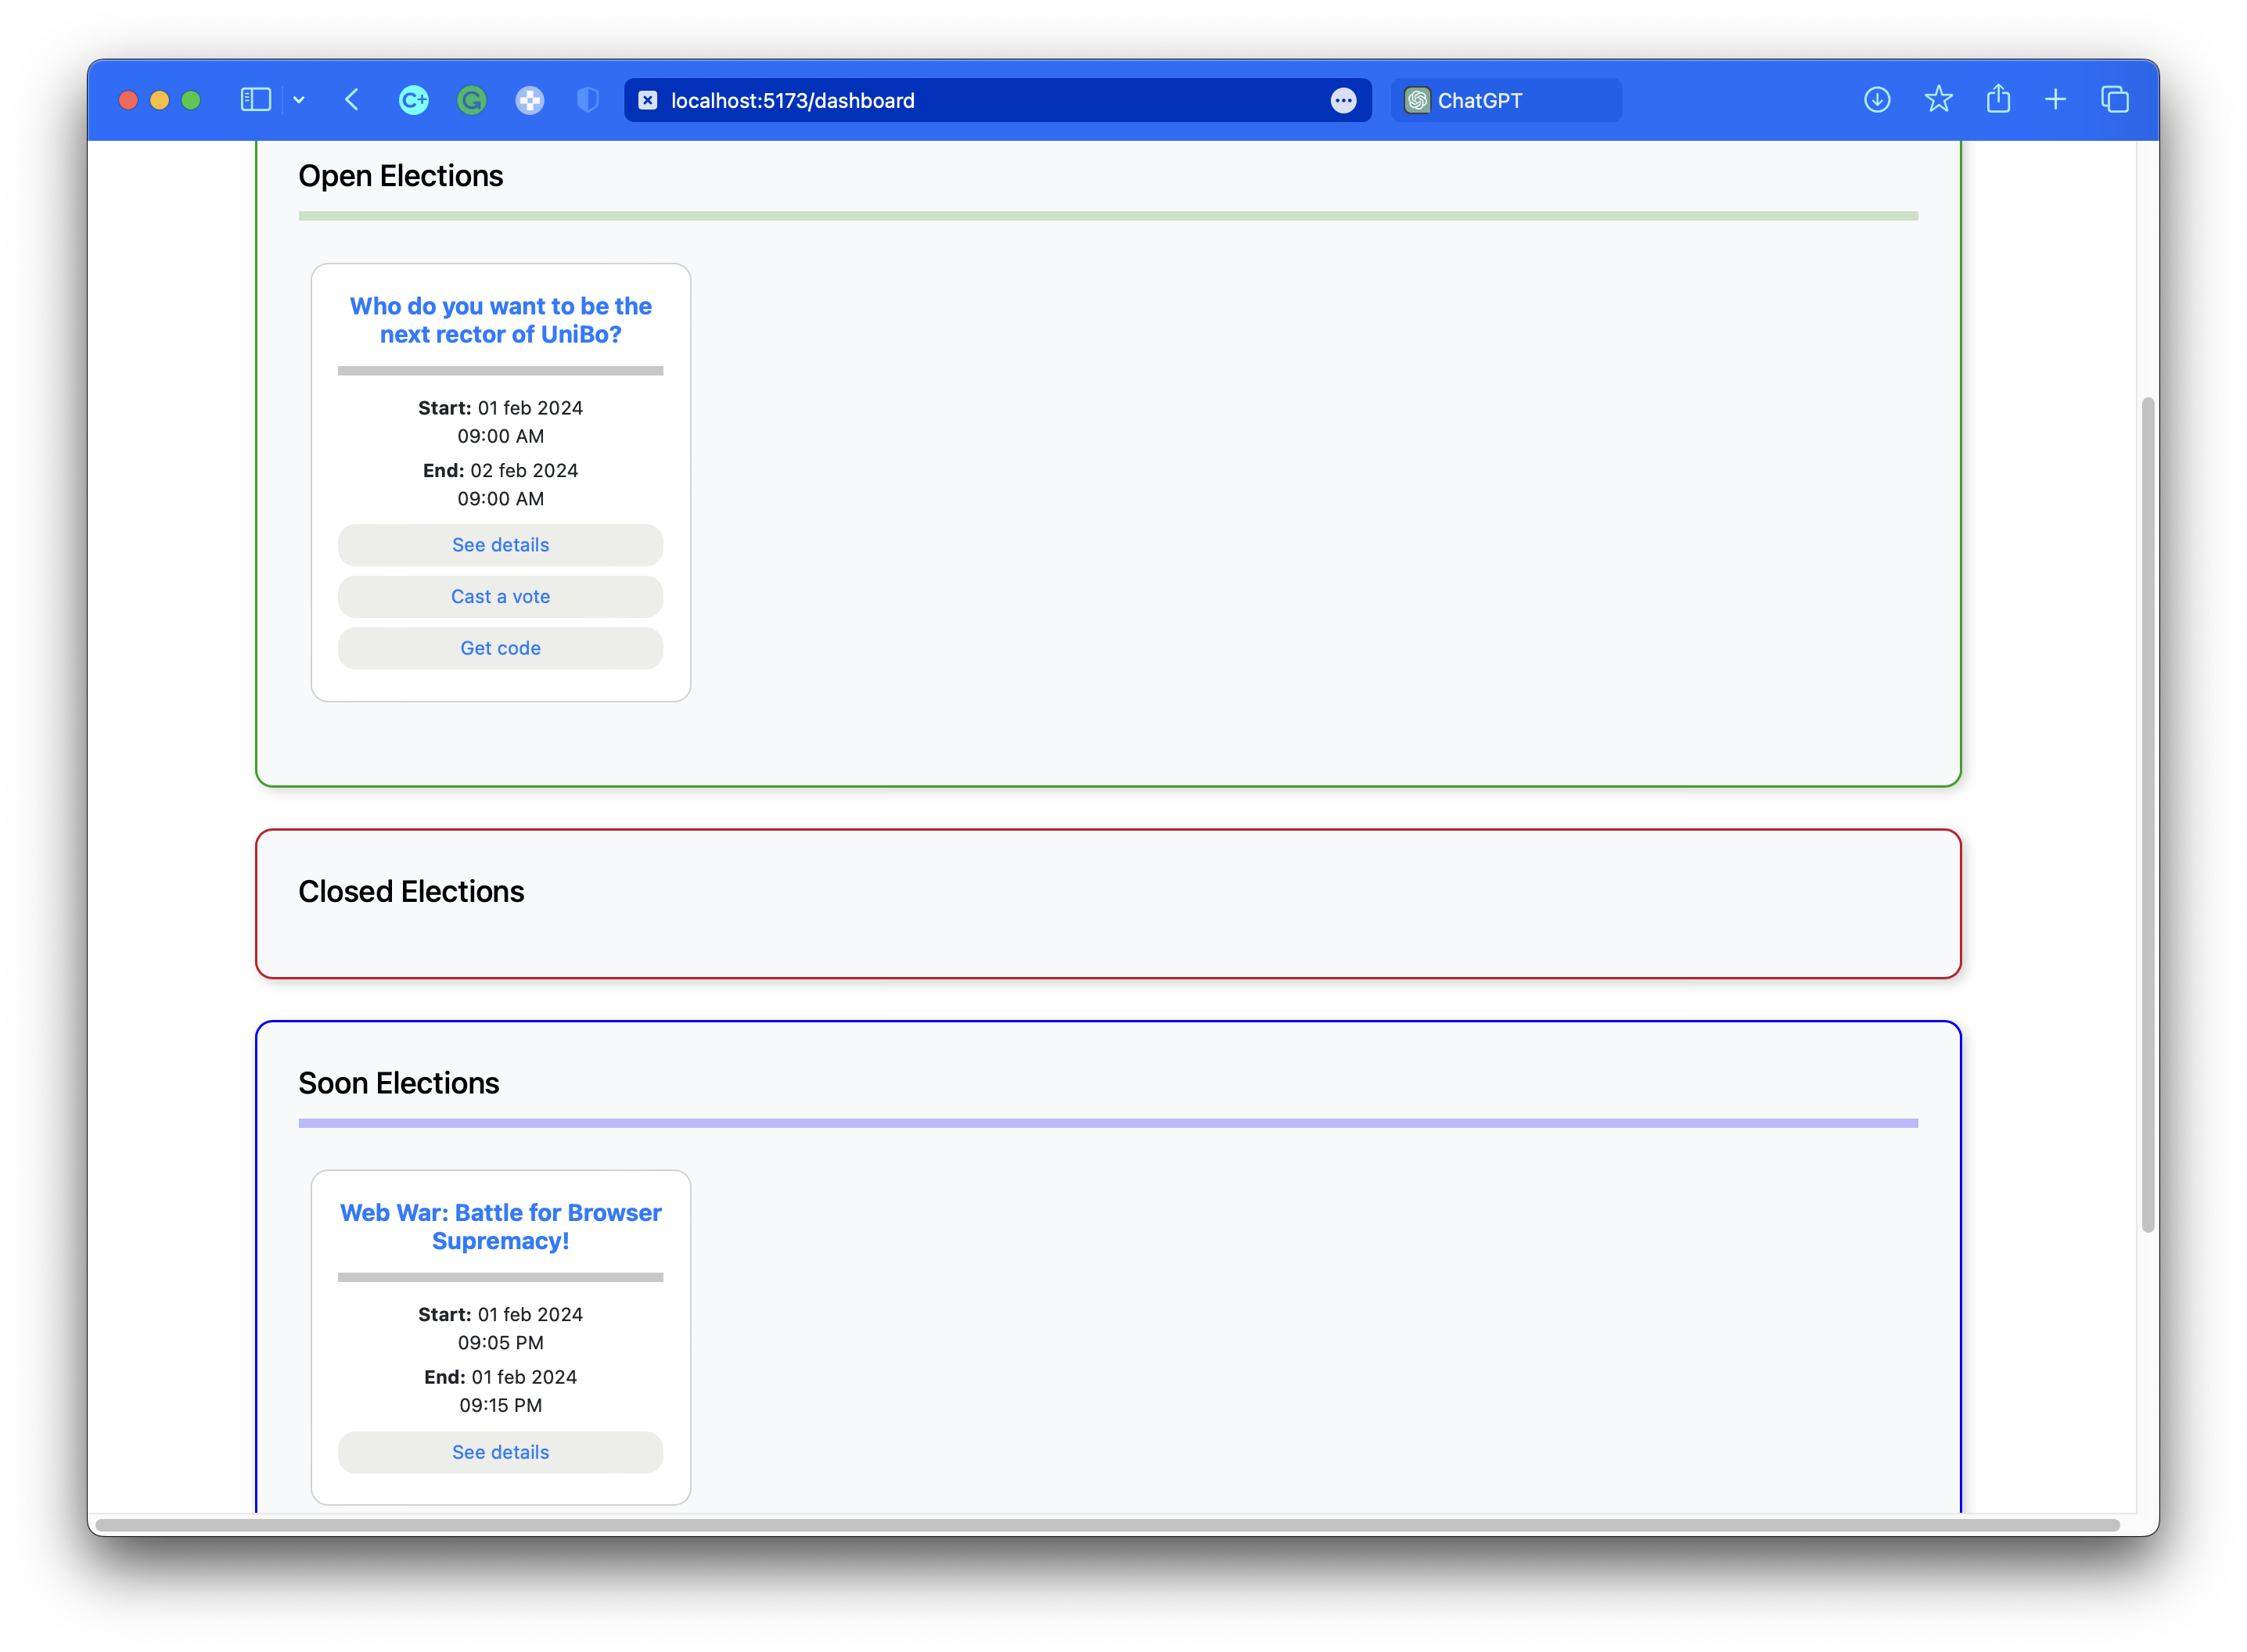
\includegraphics[width=0.9\linewidth]{figures/story-board/6-dashboard.png}
    \caption{Dashboard view.}
    \label{fig:dashboard}
\end{figure}

\begin{figure}
    \centering
    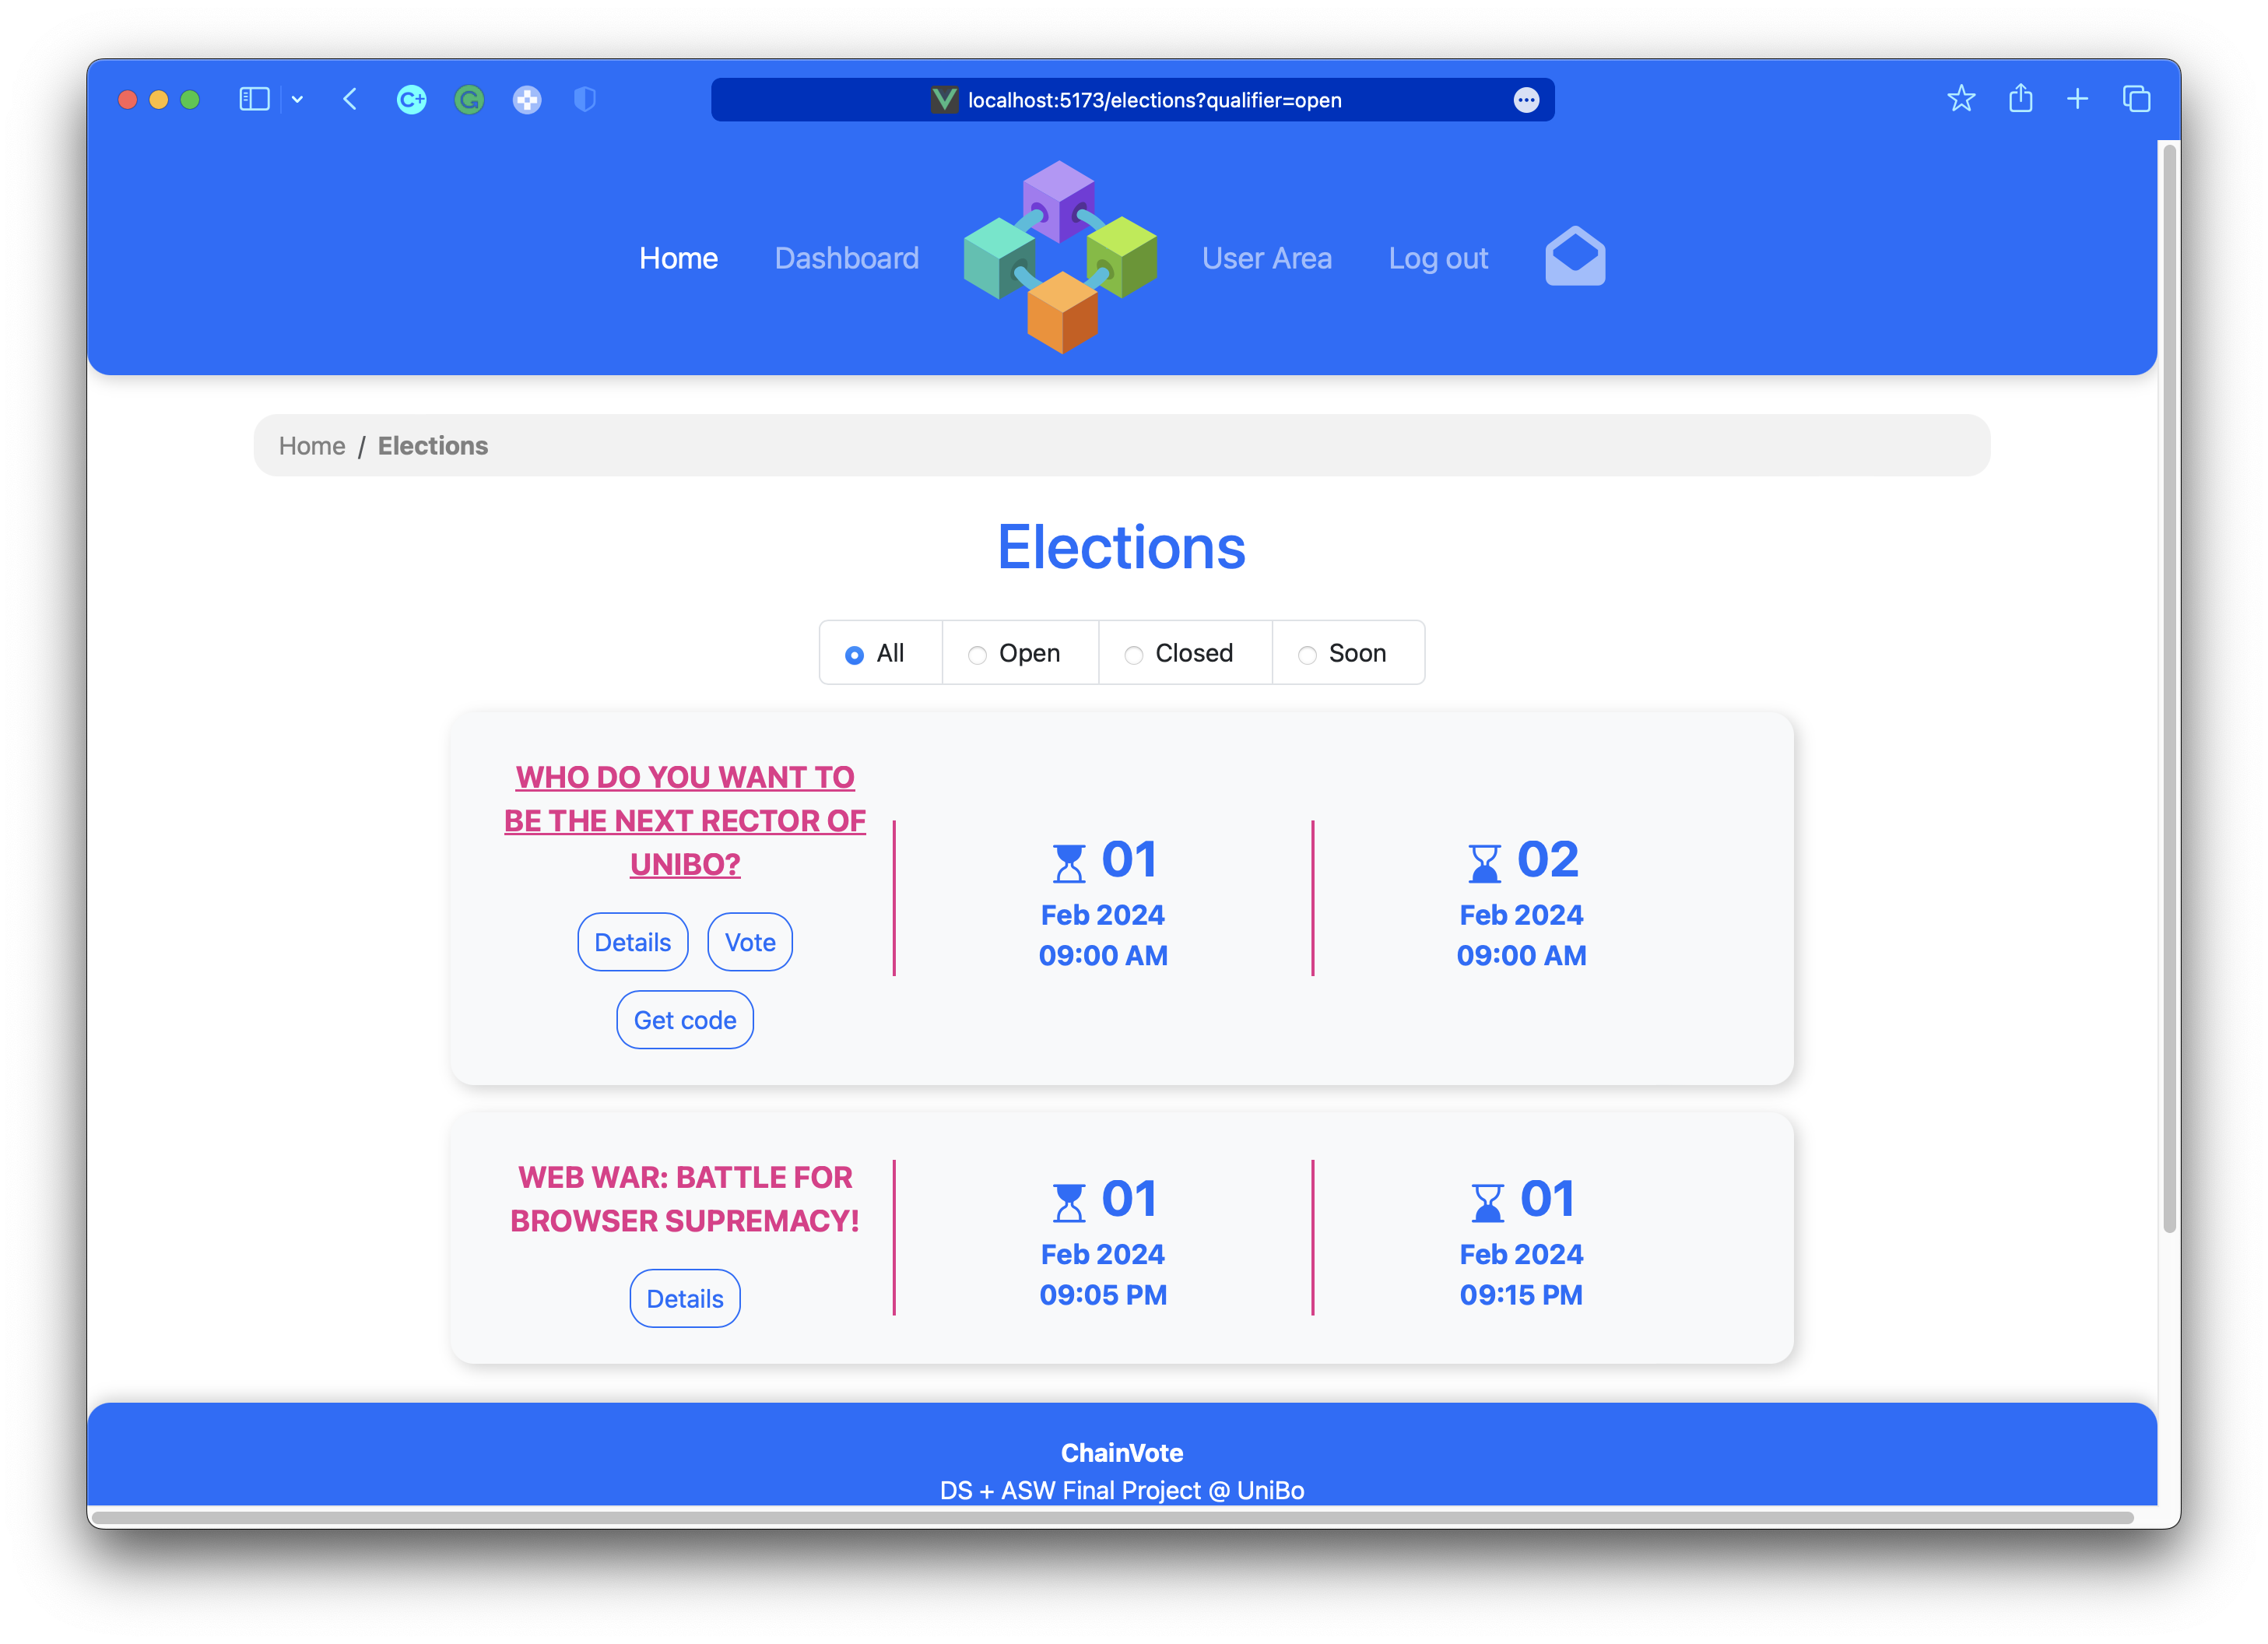
\includegraphics[width=0.9\linewidth]{figures/story-board/6a-elections.png}
    \caption{Elections list view.}
    \label{fig:elections}
\end{figure}

\begin{figure}
    \centering
    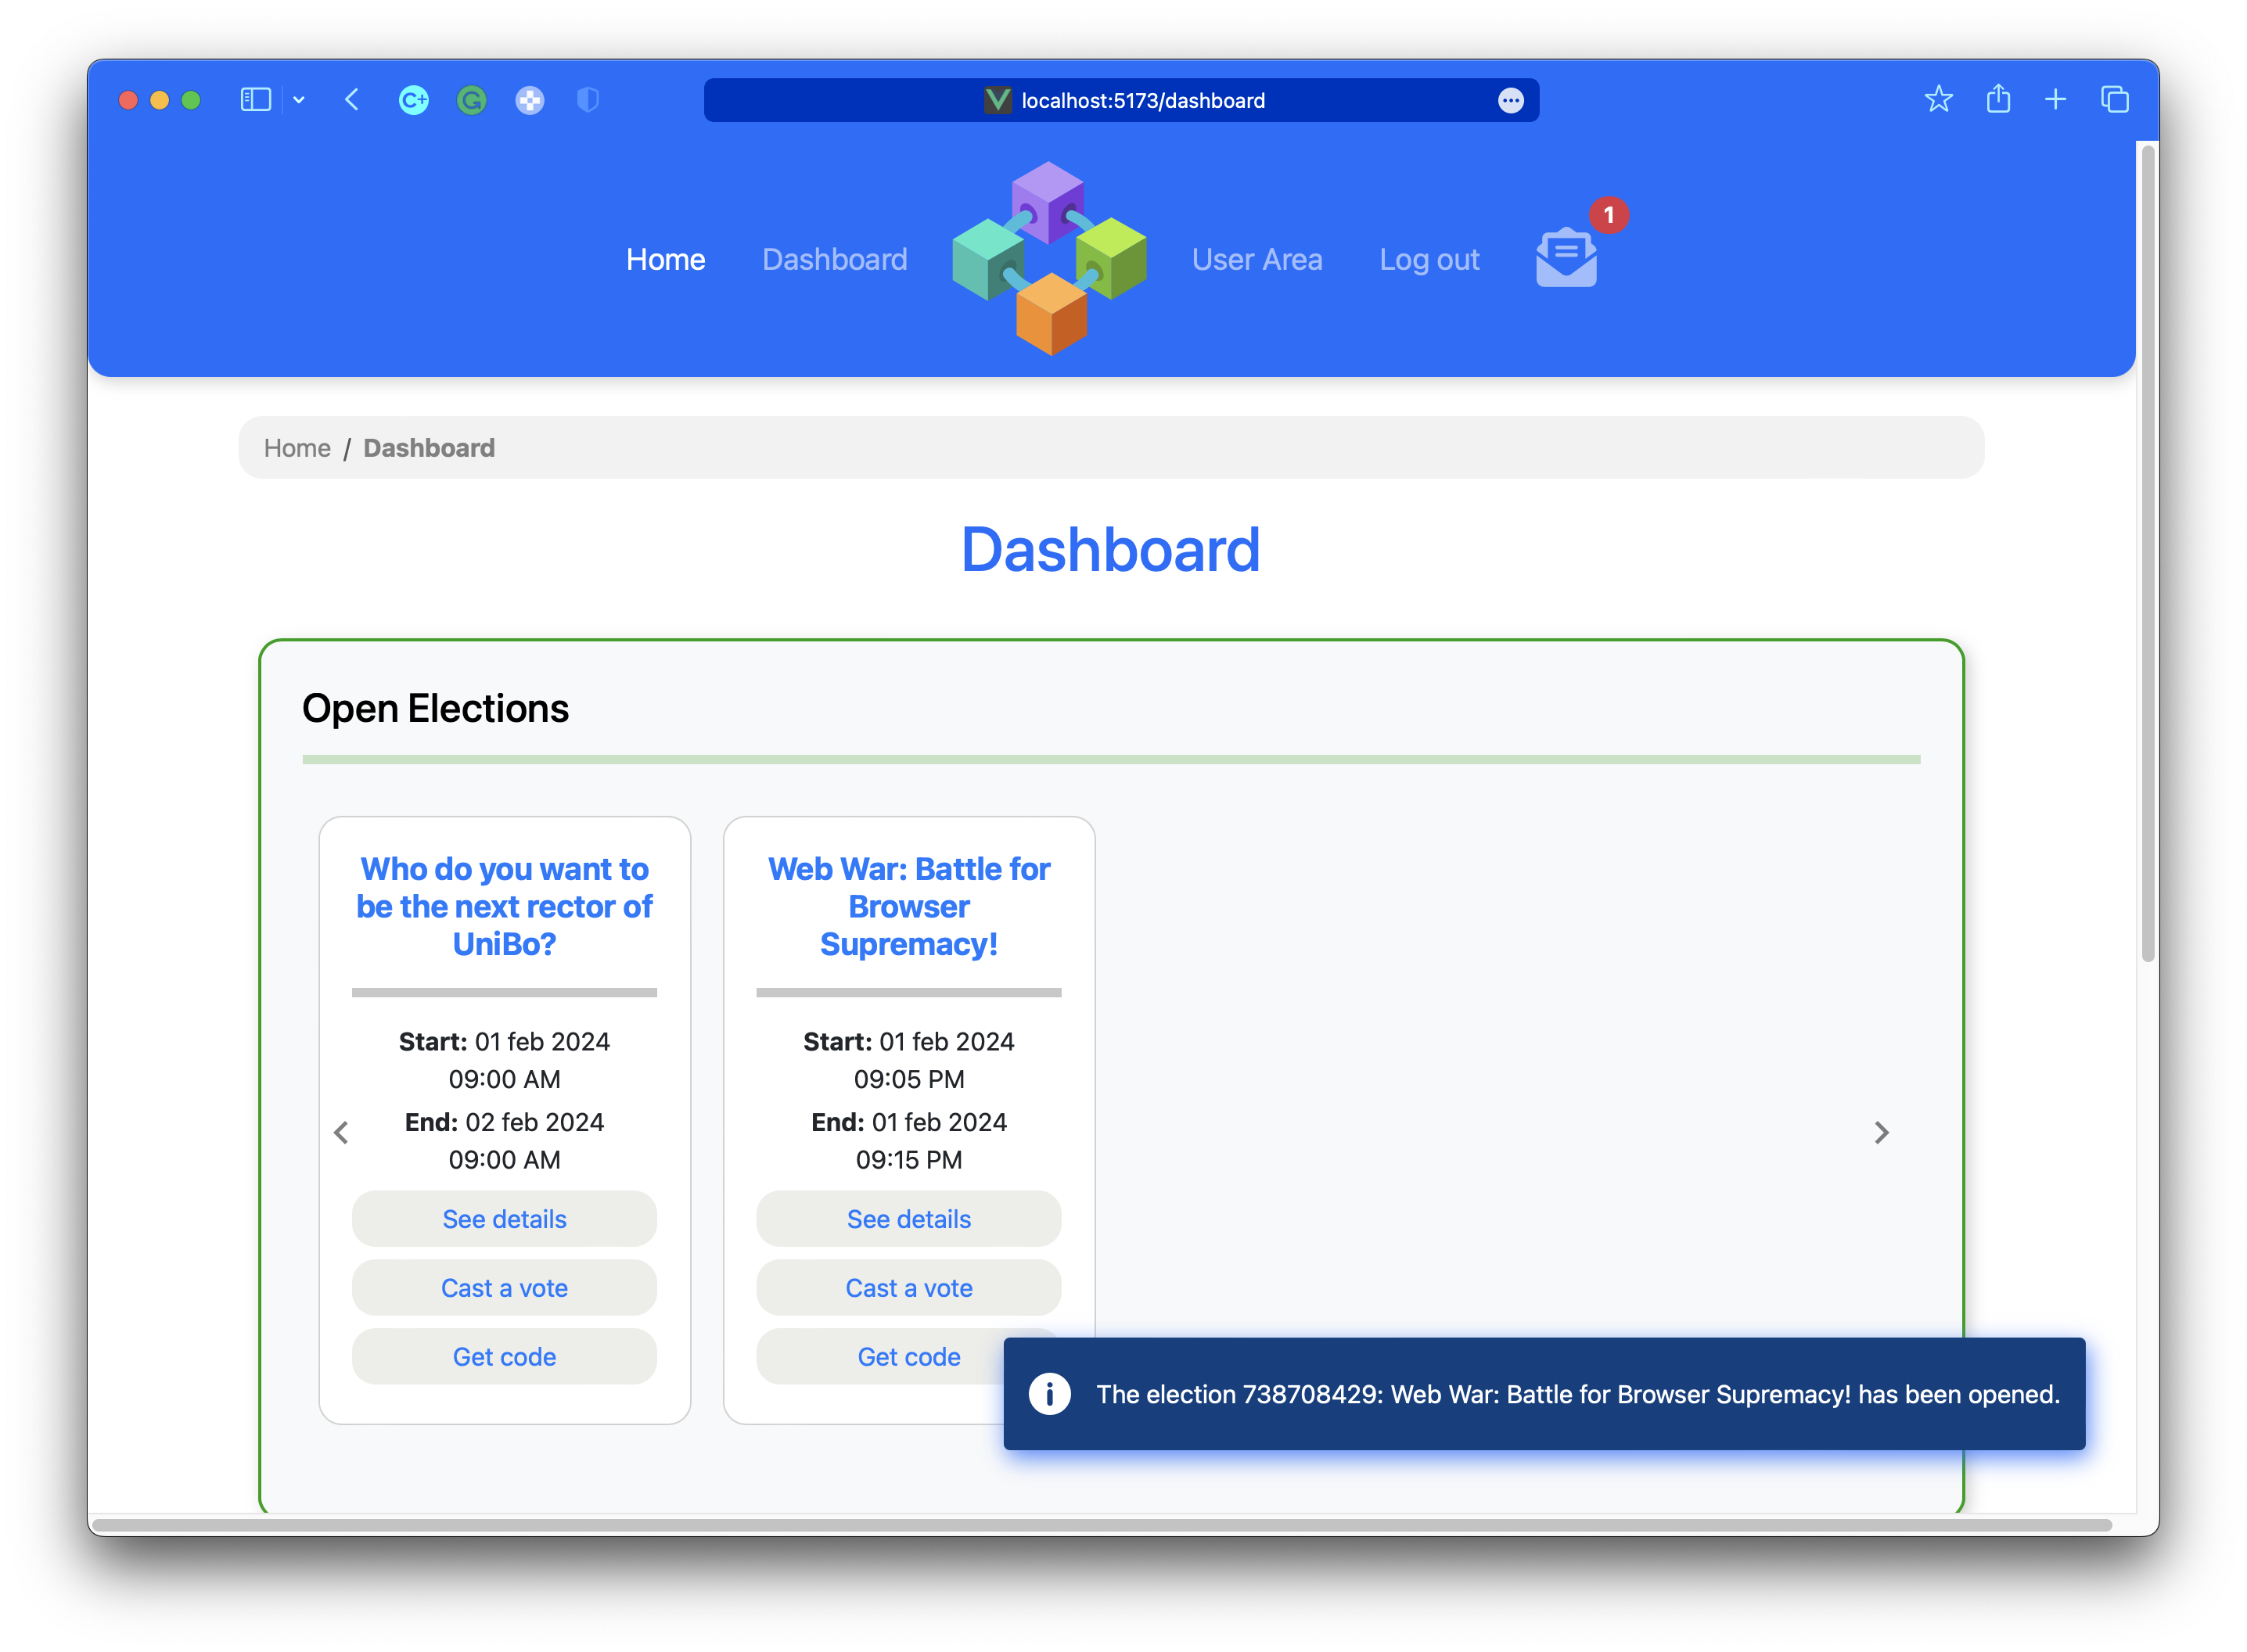
\includegraphics[width=0.9\linewidth]{figures/story-board/8-notifications.png}
    \label{fig:notifications}
    \caption{A toast notification pops up and the election card is updated.}
\end{figure}
\restoregeometry

Once the election opens the user is notified by a toast message which appears and the notification icon in the navbar is updated to reflect the number of new notification not yet read (\Cref{fig:notifications}).
%
At the same time the card of the election moves to the open elections section and buttons for casting a new vote are displayed.

Clicking on "Get code" a modal pops up allowing to request a one time code for that election (\Cref{fig:request-code}).
%
The first part of the code is displayed in the input field.
%
The second part is sent to the user's email address.

Once the user receives the second part of the code it's possible to insert it in the appropriate page (\Cref{fig:insert-code}).

After the code is inserted, if it is valid, the user is redirected to the page where can cast the vote (\Cref{fig:cast-vote}).
%
After expressing the choice, the user is redirected to the details page.

\newgeometry{margin=1.0cm}
\begin{figure}
    \centering
    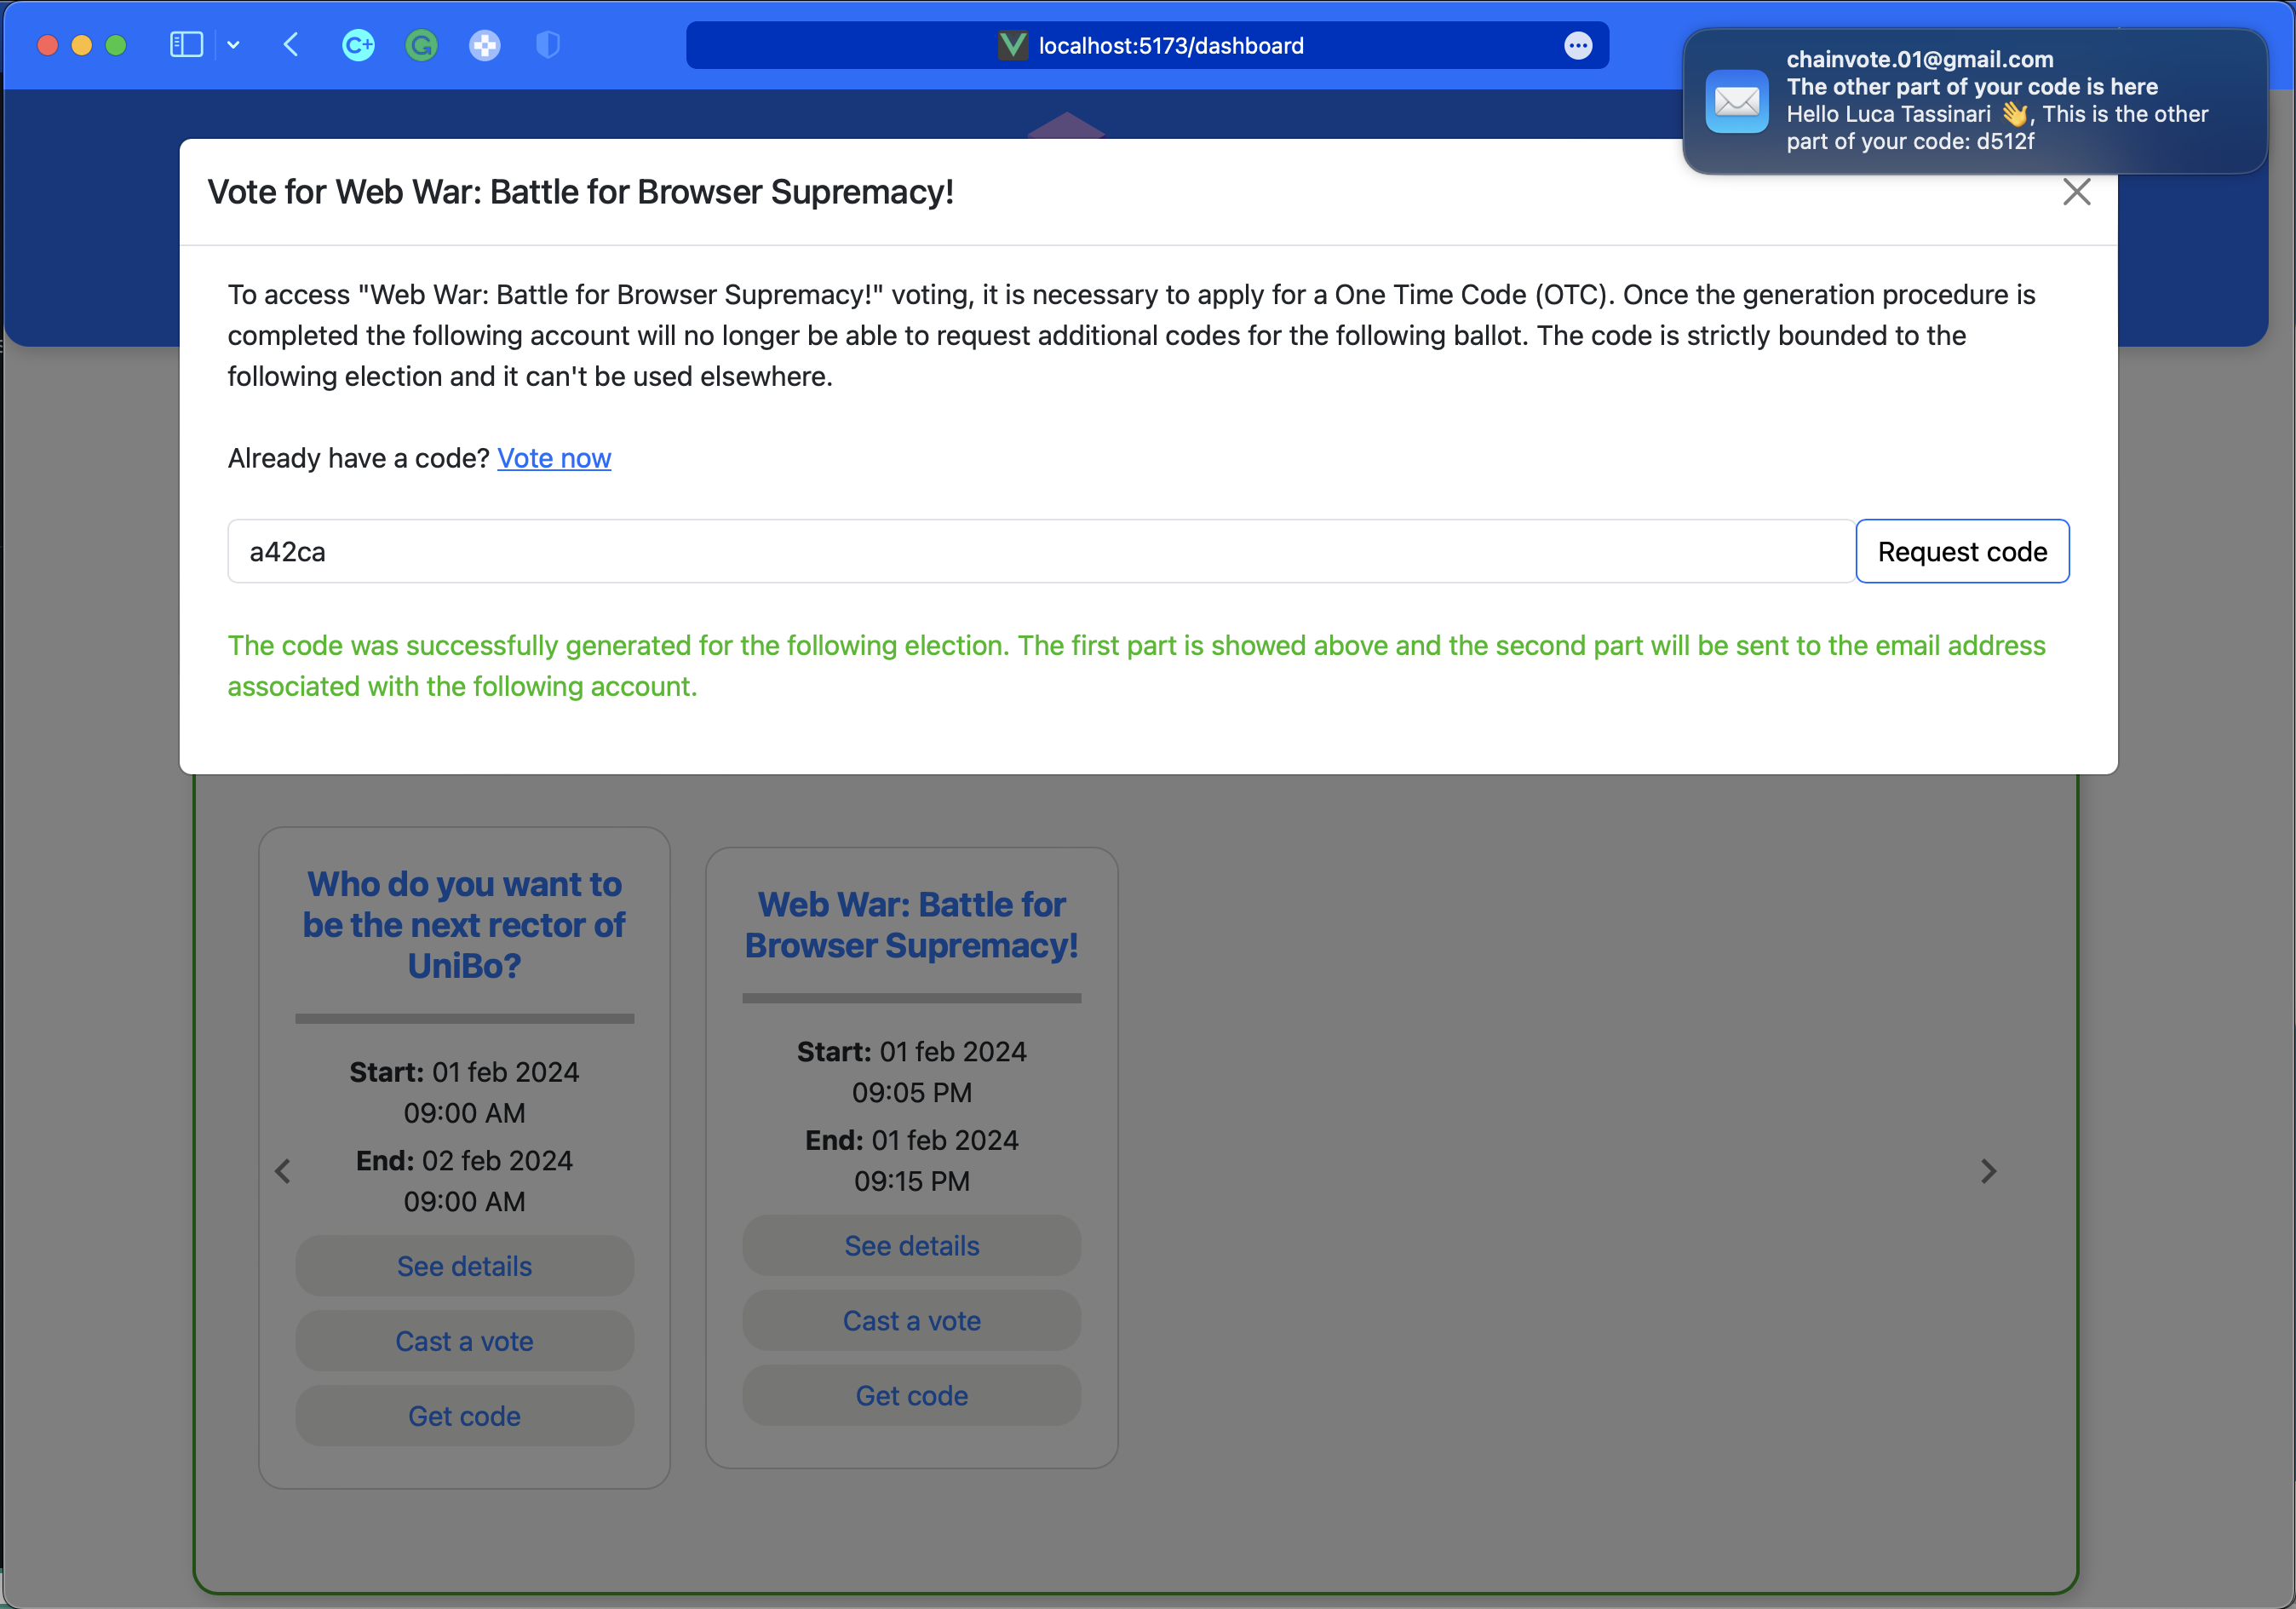
\includegraphics[width=0.8\linewidth]{figures/story-board/9-request-code.png}
    \label{fig:request-code}
    \caption{Request code modal.}
\end{figure}

\begin{figure}
    \centering
    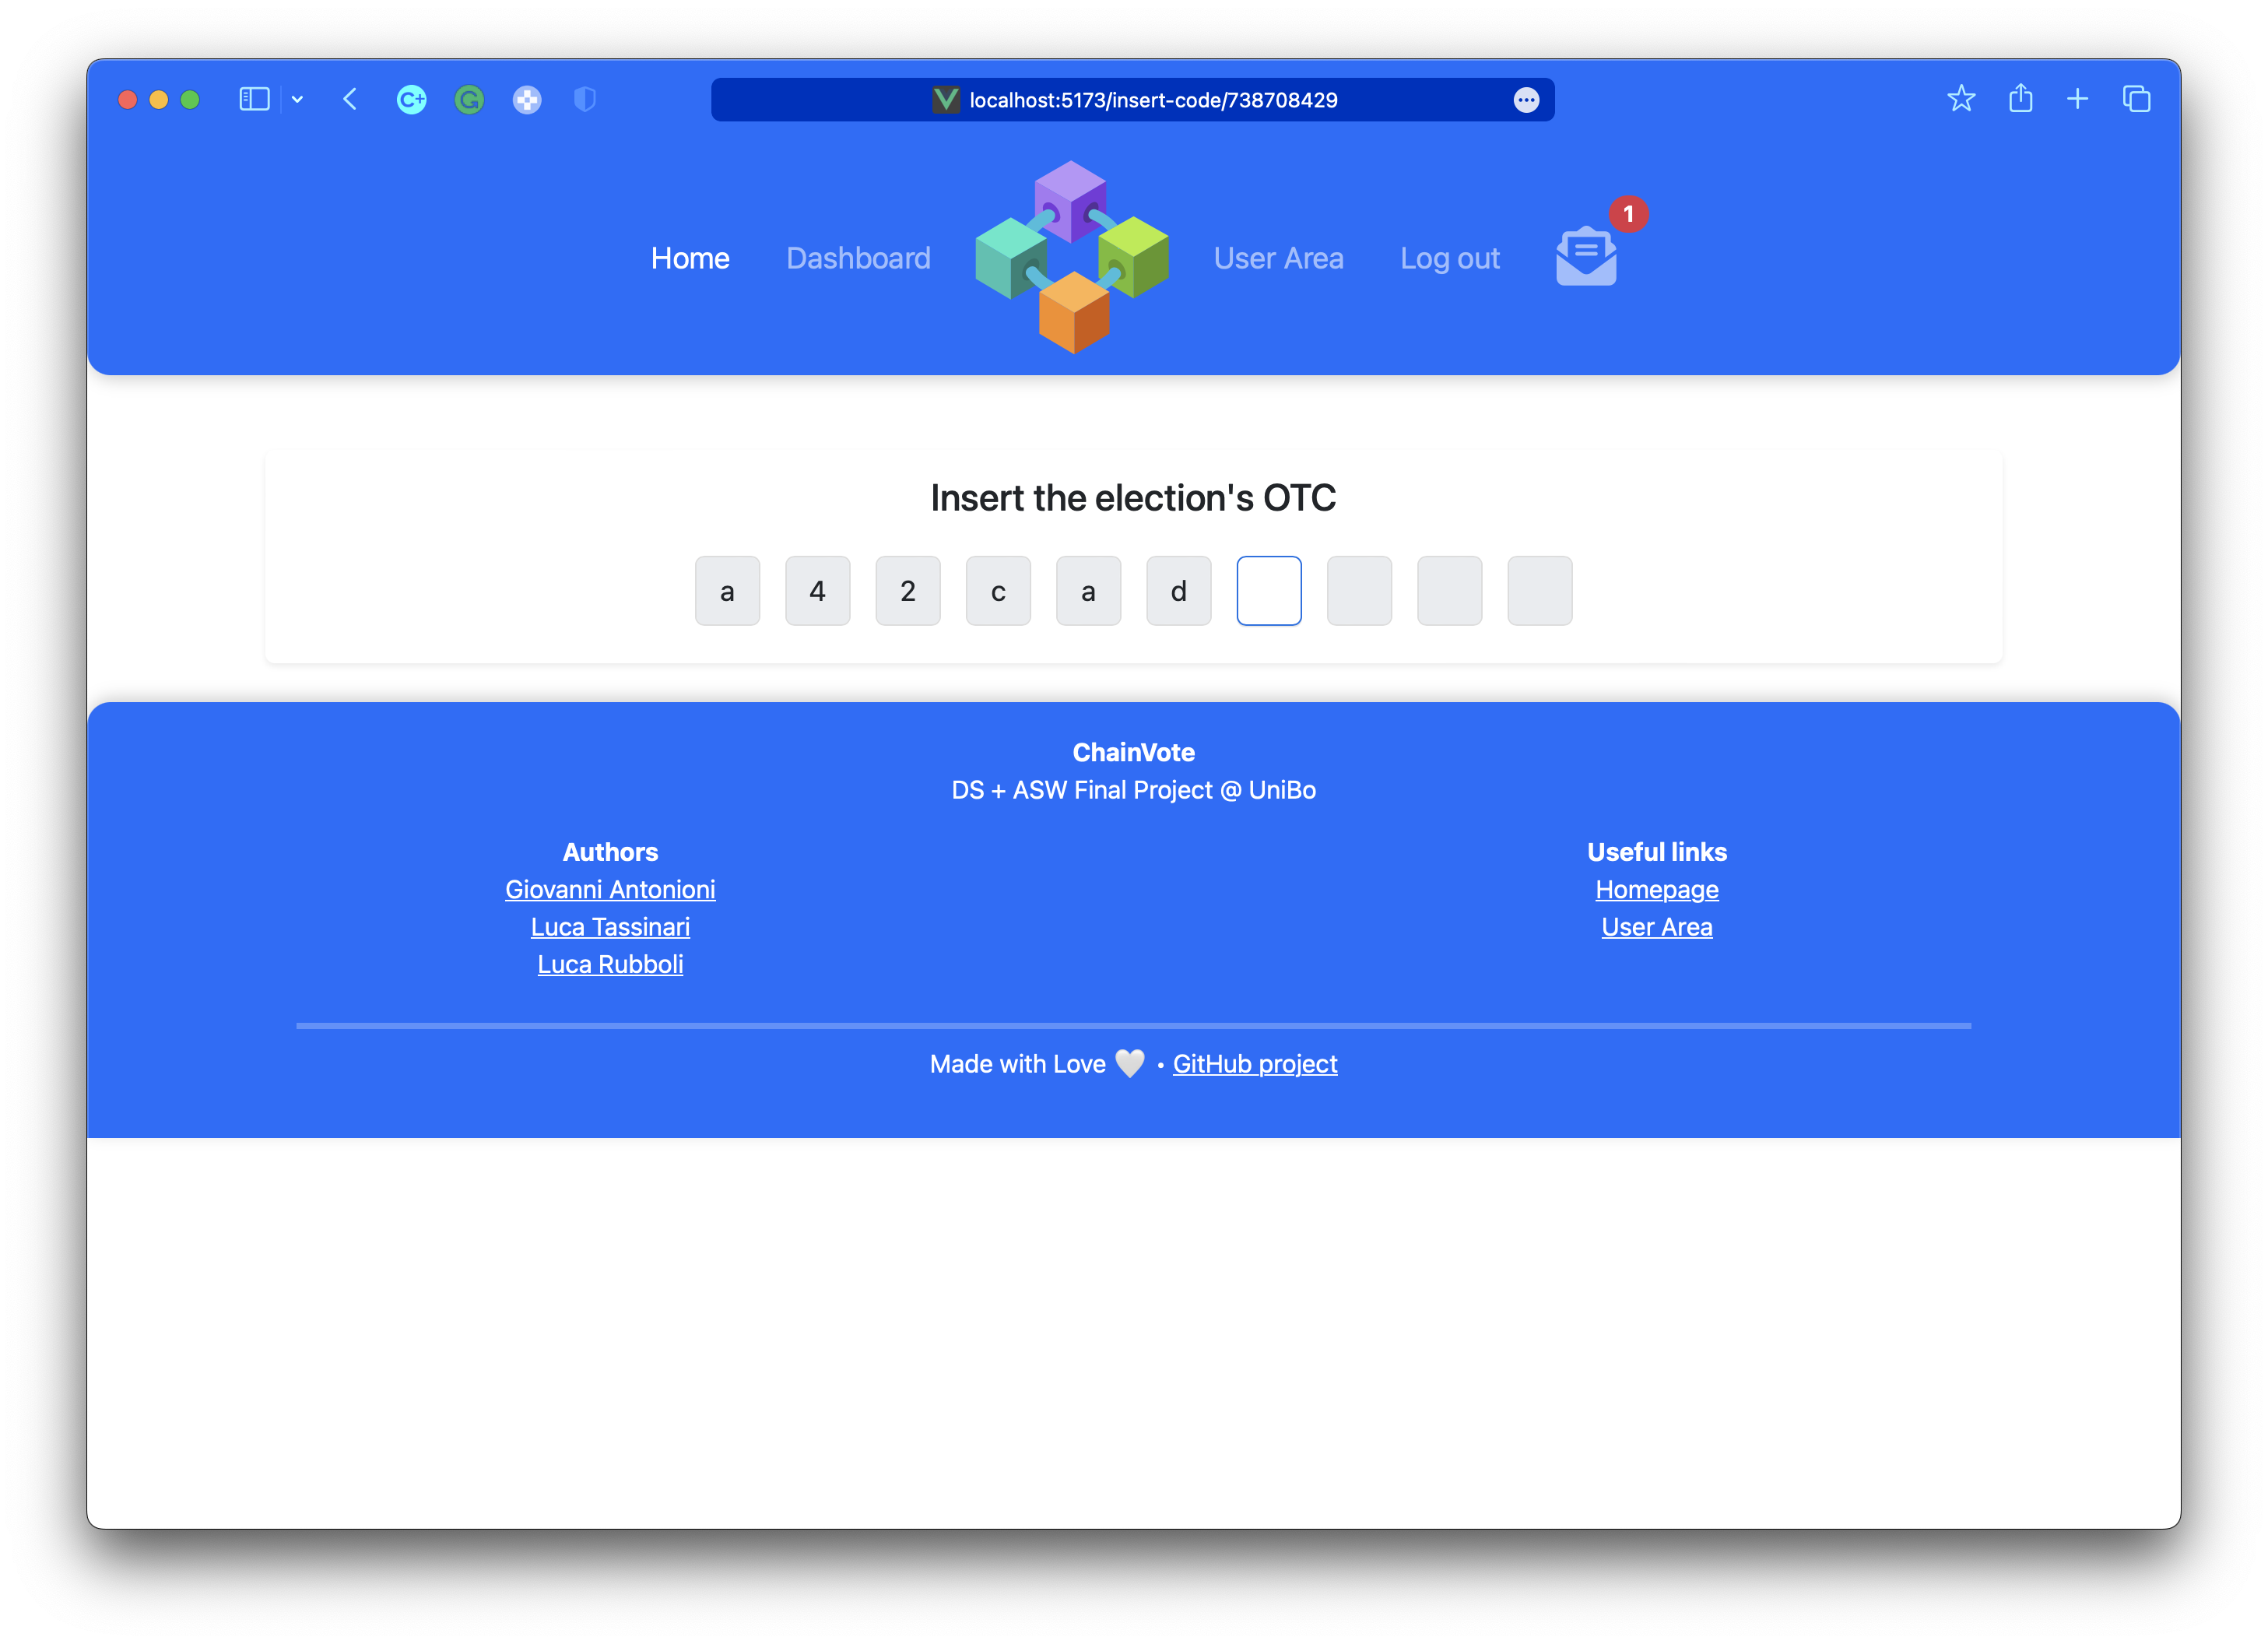
\includegraphics[width=0.9\linewidth]{figures/story-board/10-insert-code.png}
    \label{fig:insert-code}
    \caption{Insert one-time-code view.}
\end{figure}

\begin{figure}
    \centering
    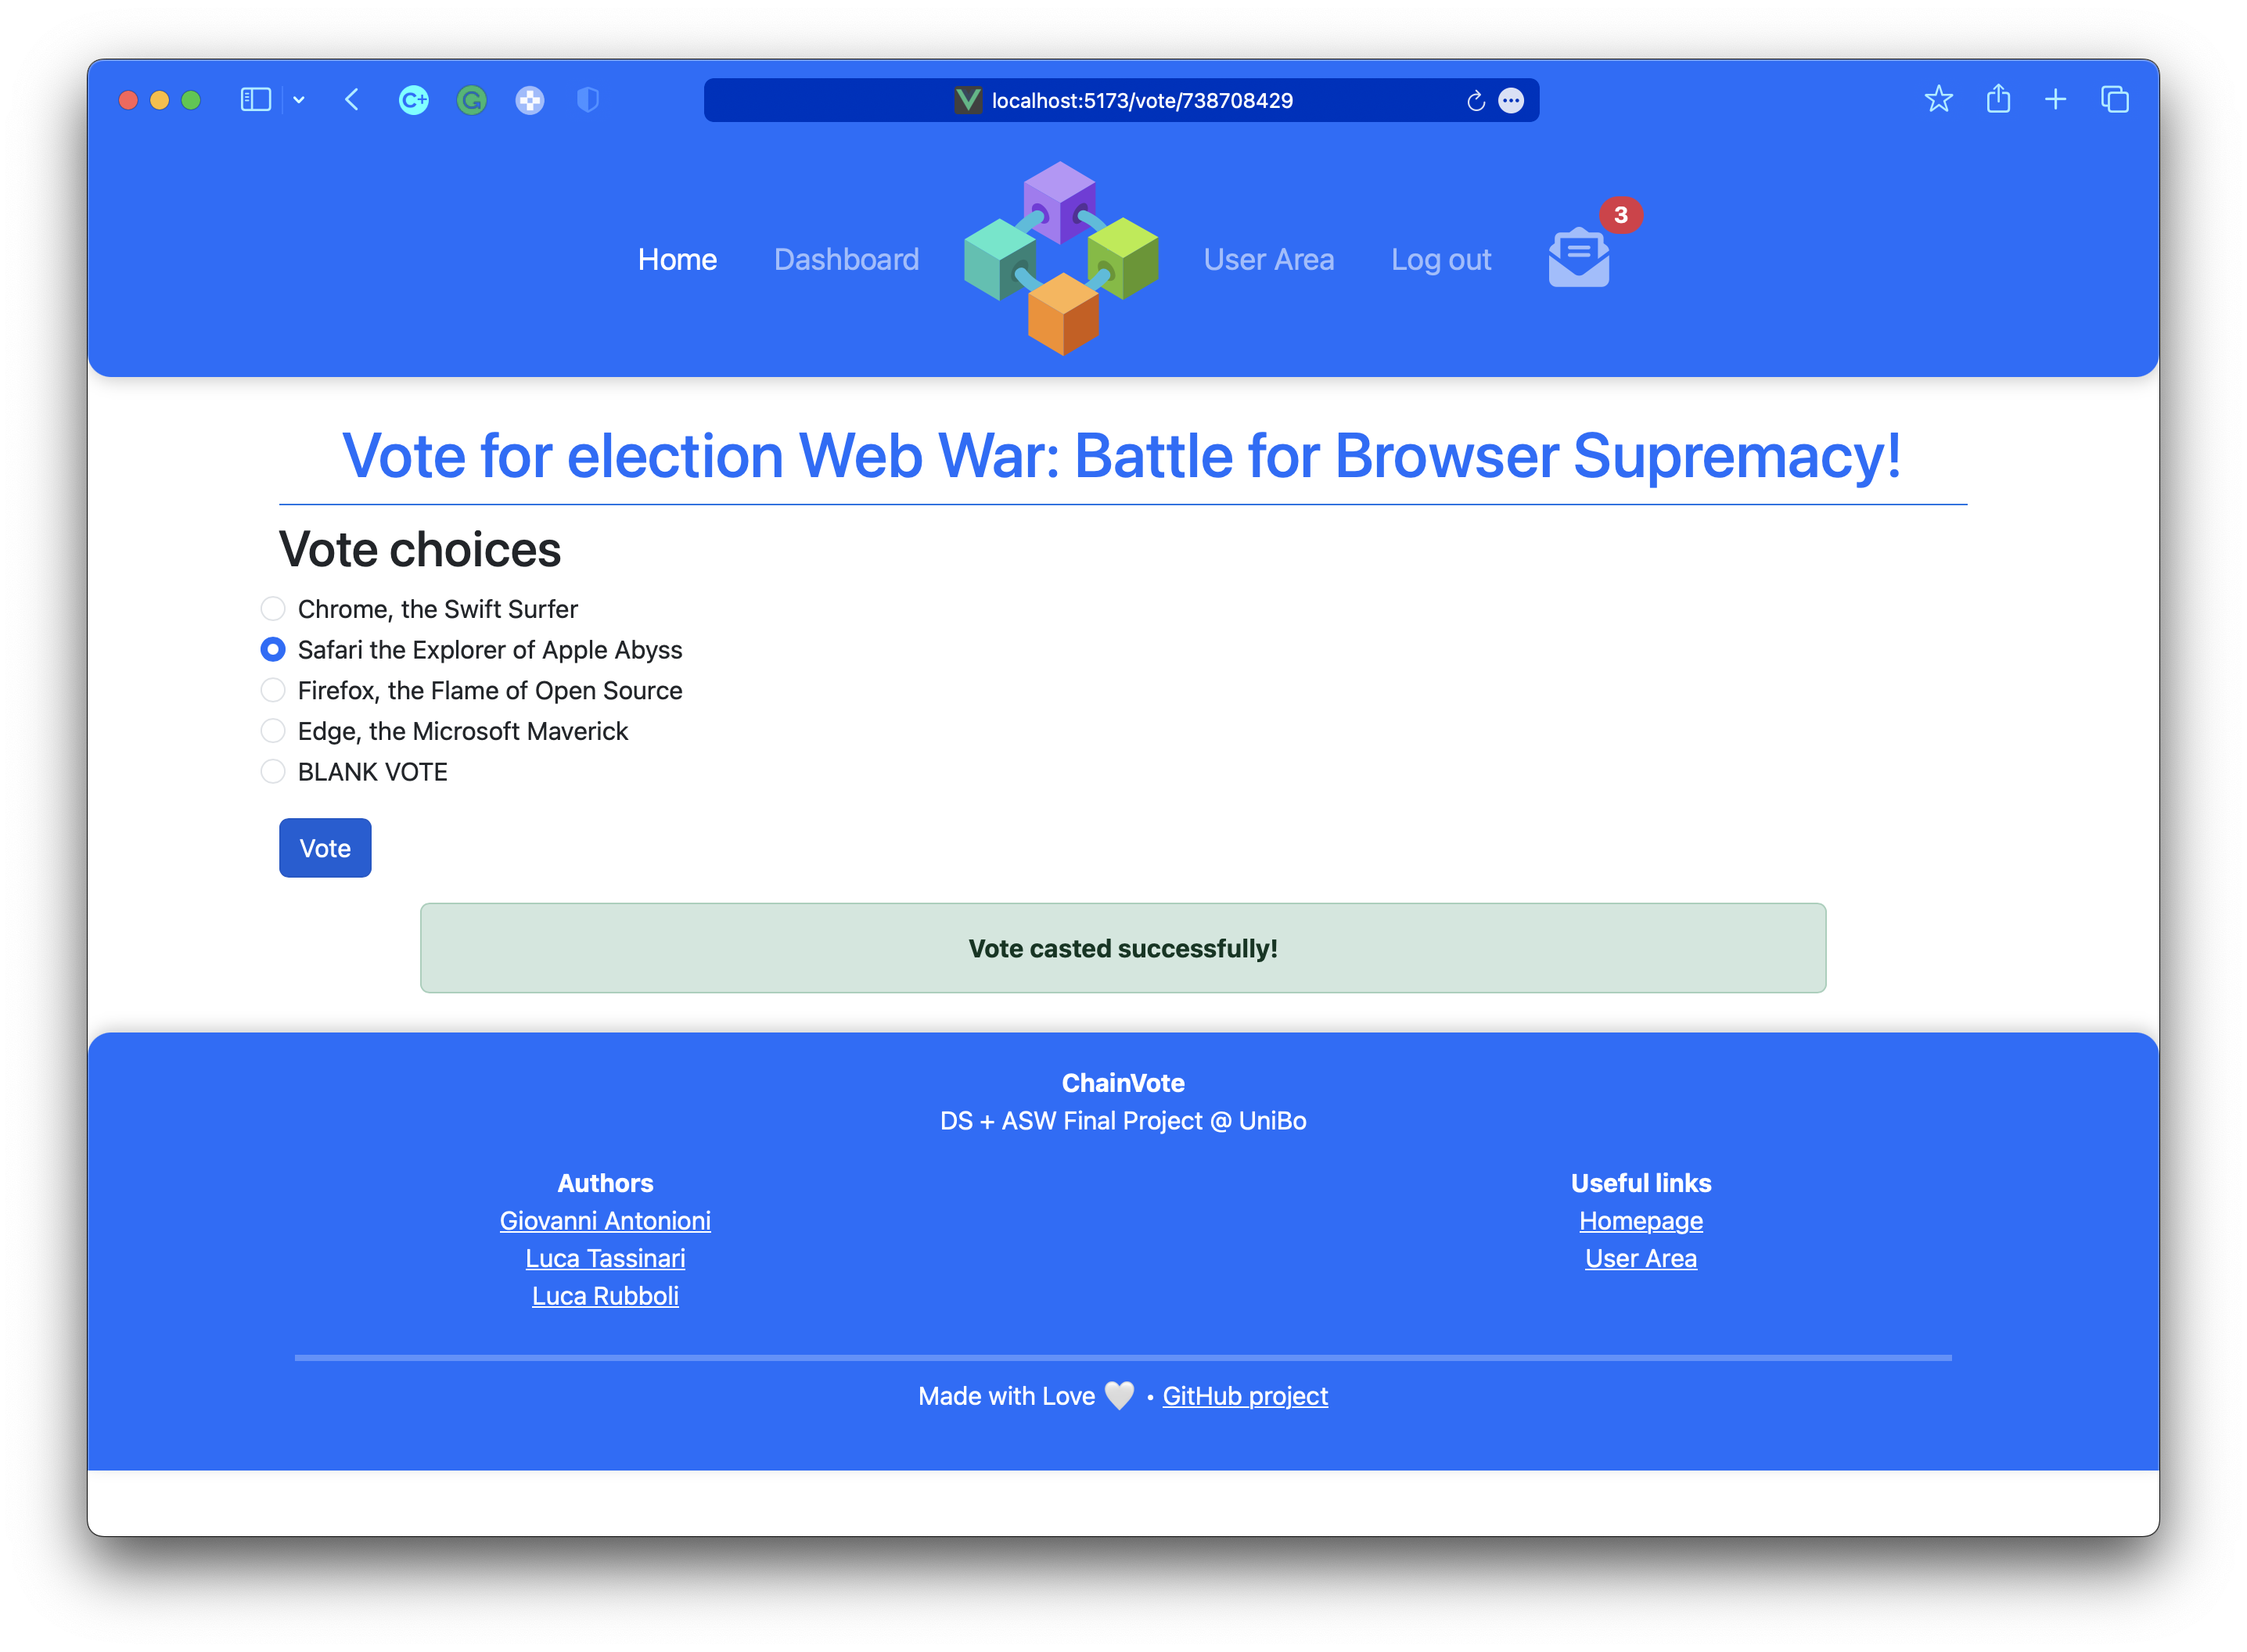
\includegraphics[width=0.9\linewidth]{figures/story-board/11-cast-vote.png}
    \caption{Vote casting view.}
    \label{fig:cast-vote}
\end{figure}

\begin{figure}
    \centering
    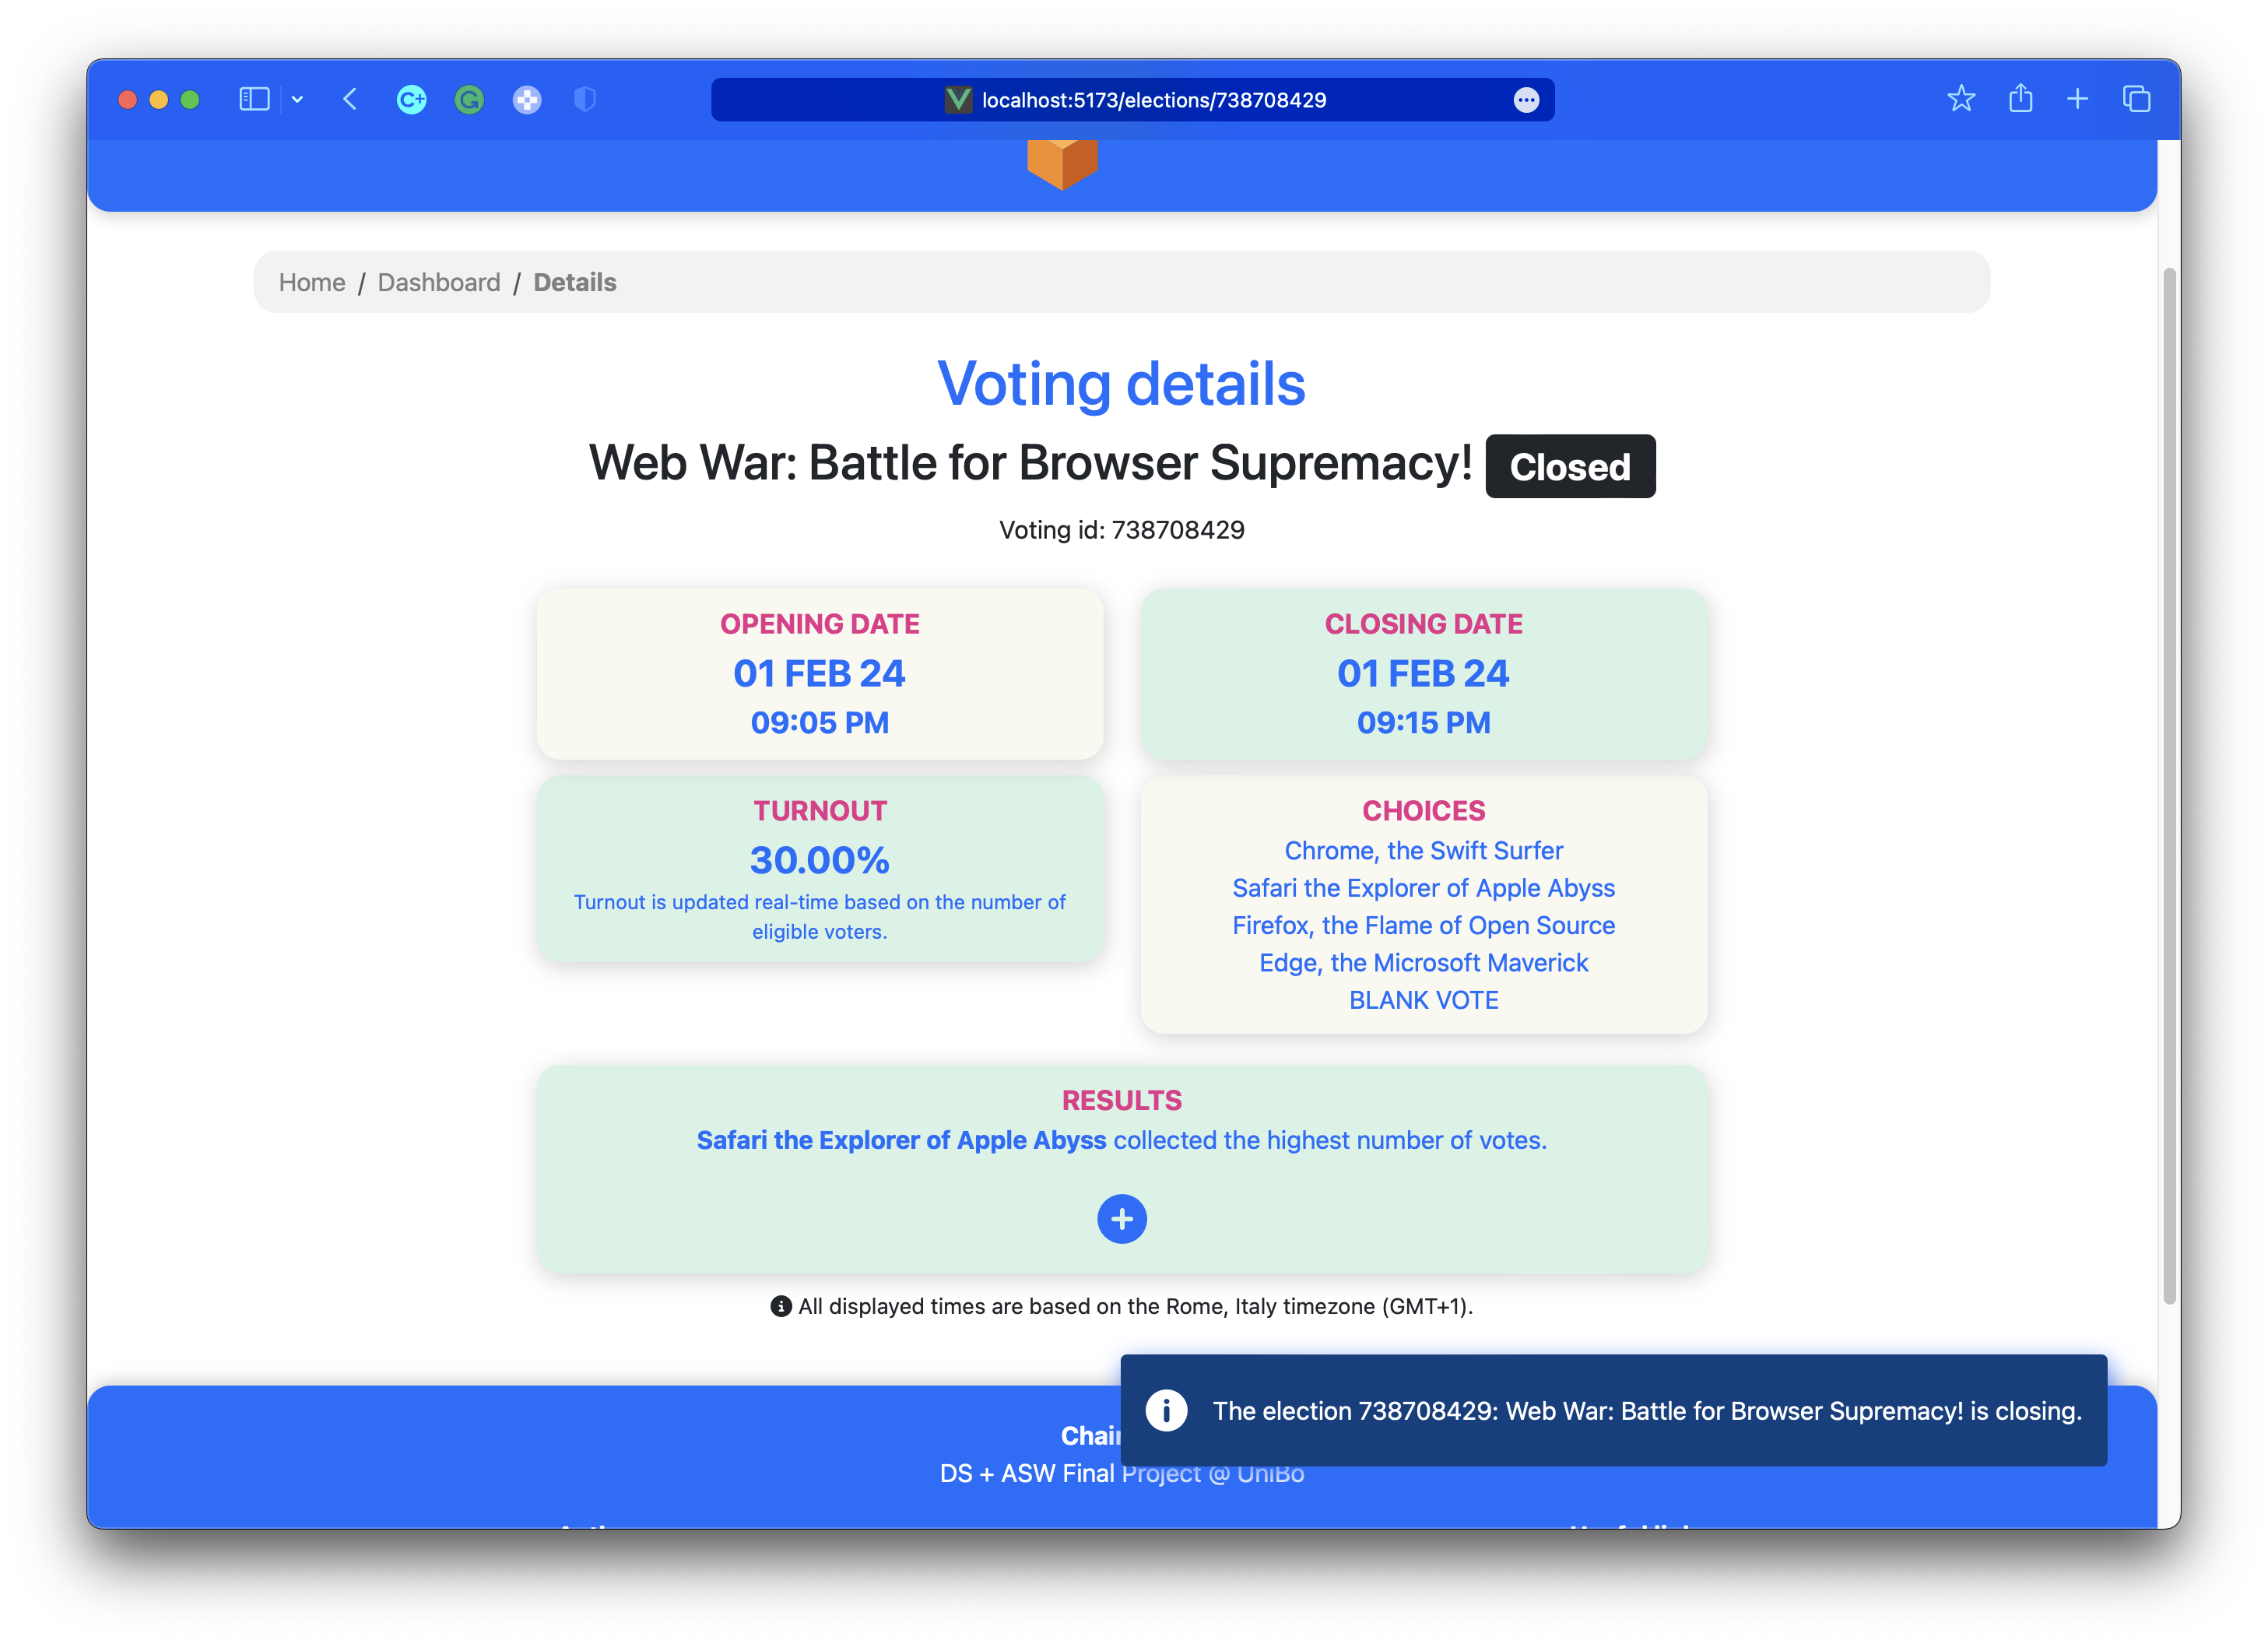
\includegraphics[width=0.9\linewidth]{figures/story-board/12-details.png}
    \caption{Election details view.}
    \label{fig:details}
\end{figure}
\restoregeometry

The details page shows all the information about the election: the static ones along with the turnout (updated in real time) and the results, which are displayed only after the election is closed (\Cref{fig:details}).
%
For brevity's sake, the page shows both the notification toast alerting the user the election is closing (which is sent some time before the closing time) and the look of the page once the election is closed.

Results are displayed both tabularly and graphically by means of both a pie chart and a bar chart (\Cref{fig:results-1}, \Cref{fig:results-2}).

In any moment the user can read the received notifications by clicking on the notification icon in the navbar (\Cref{fig:notifications-list}).

\newgeometry{margin=1.0cm}
\begin{figure}
    \centering
    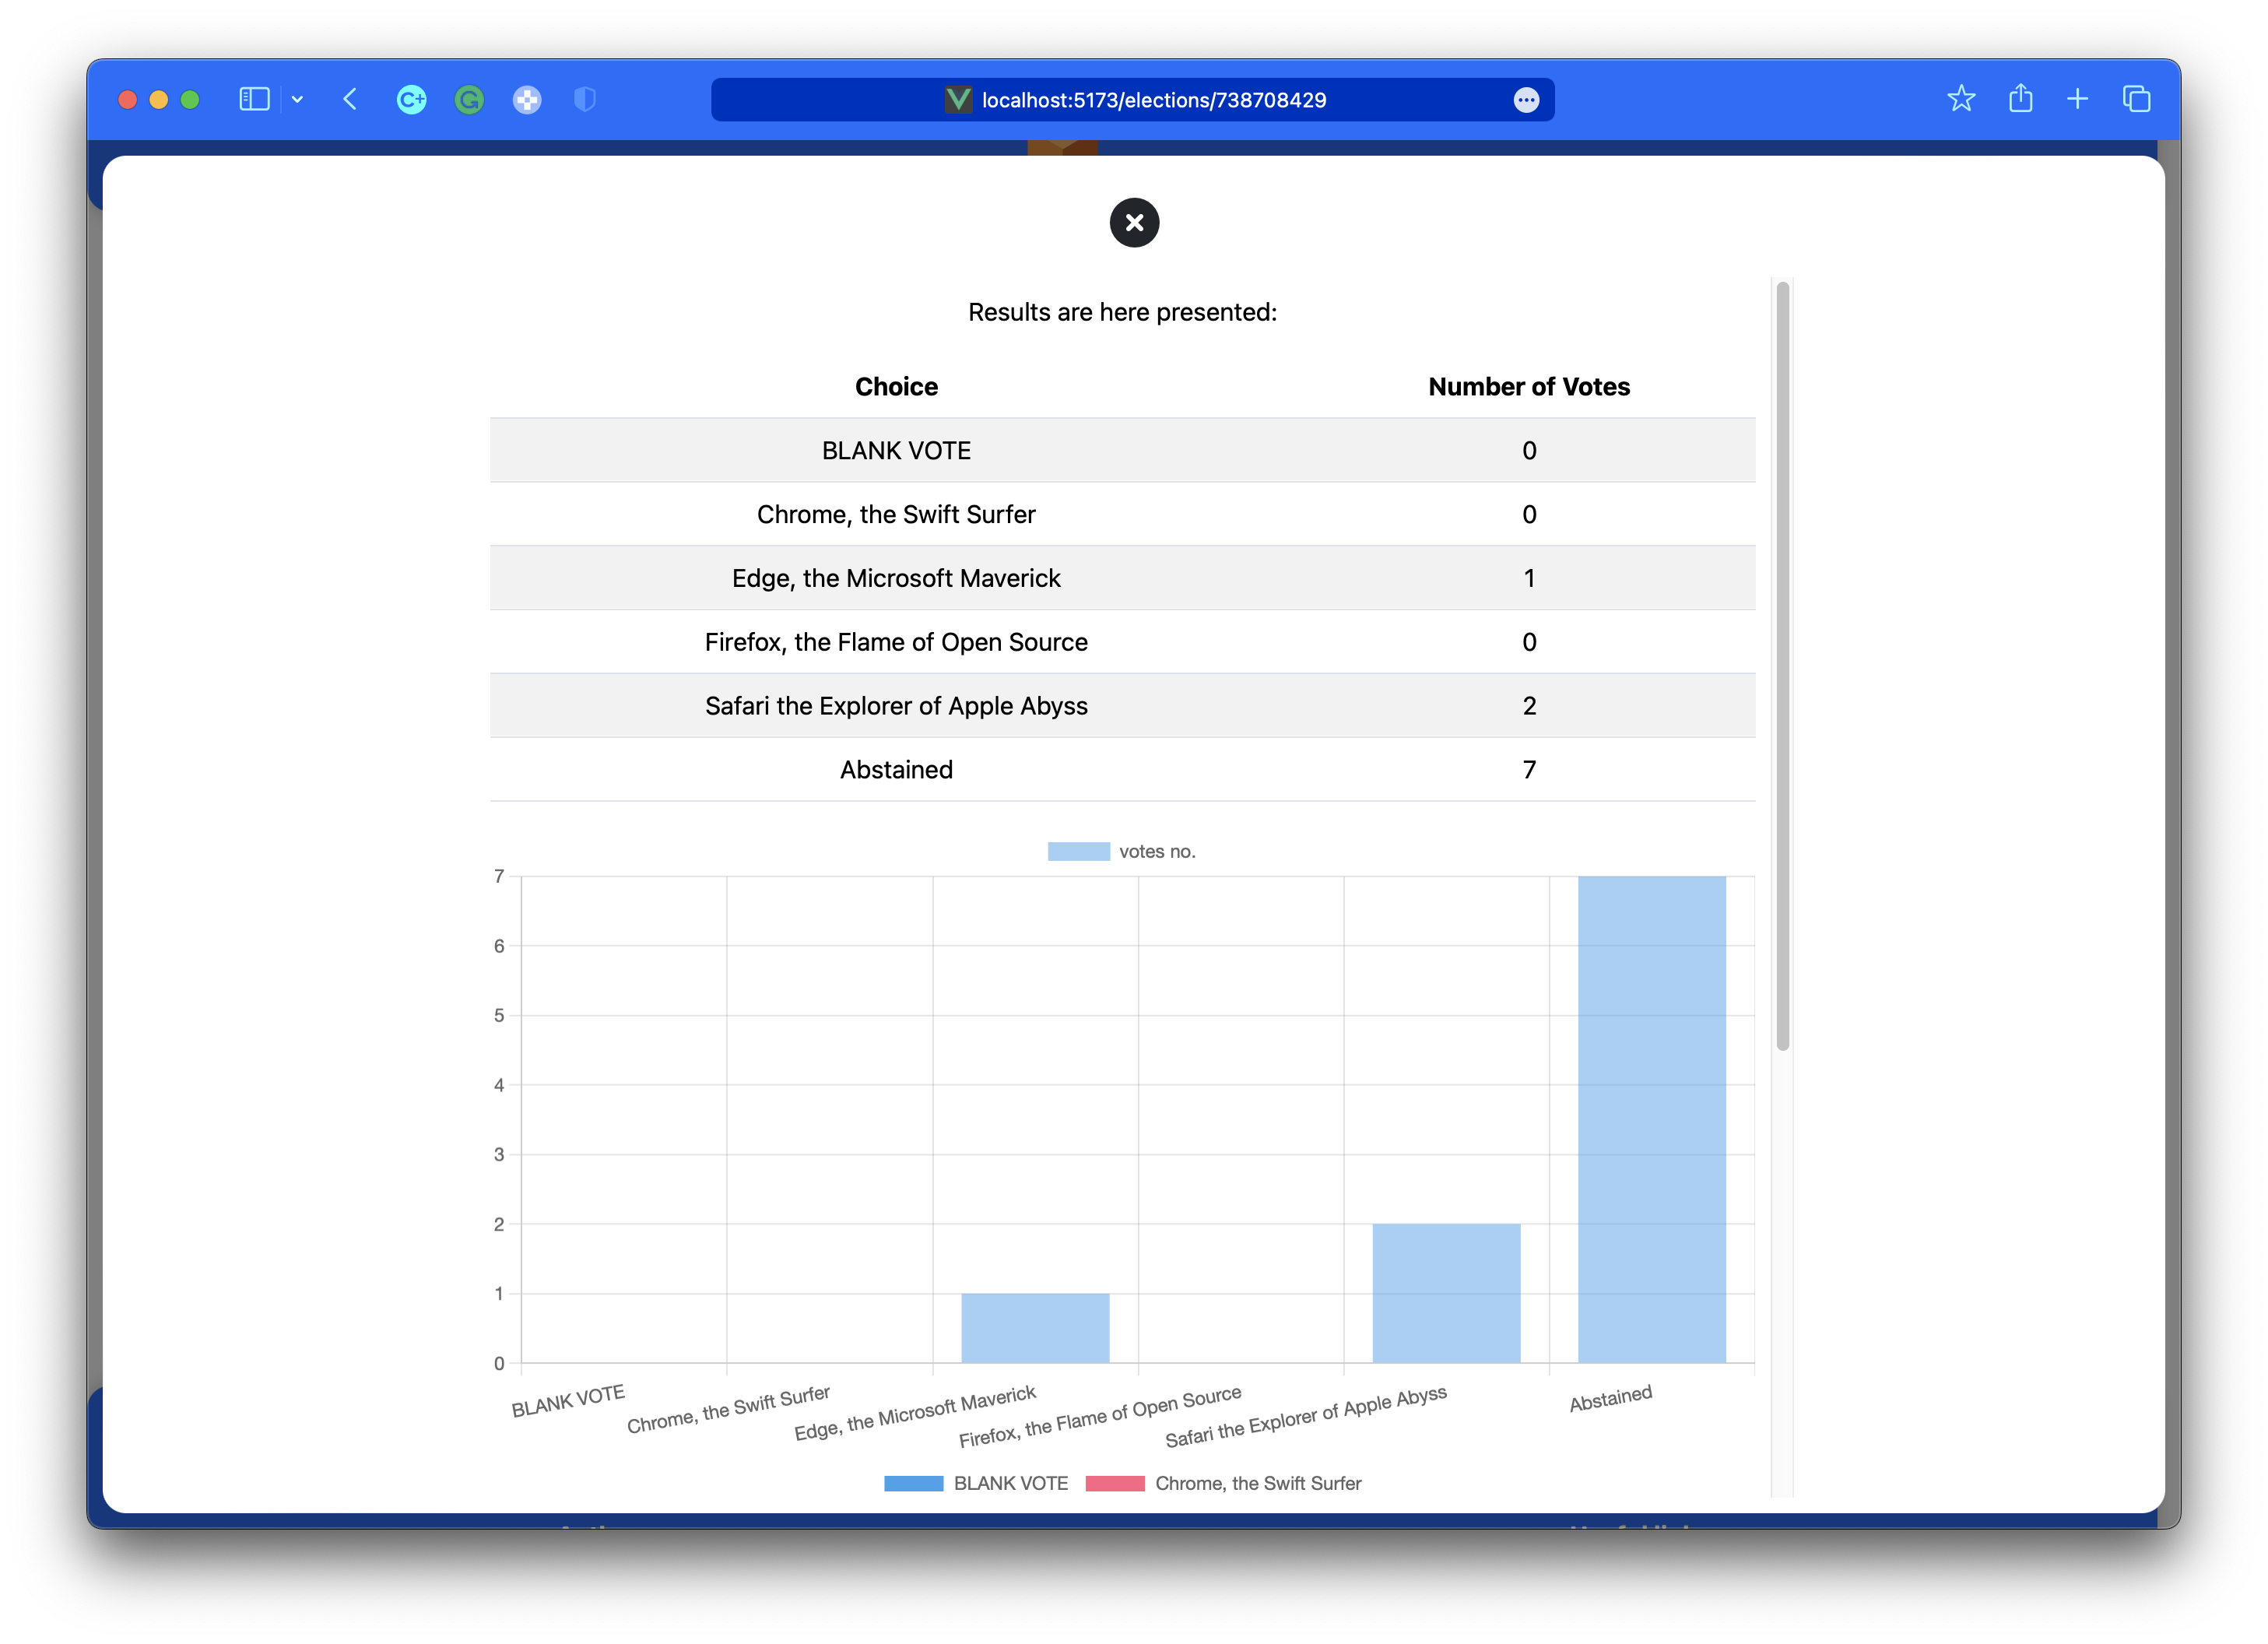
\includegraphics[width=0.9\linewidth]{figures/story-board/13-results.png}
    \label{fig:results-1}
    \caption{Election results view: table and bar chart.}
\end{figure}

\begin{figure}
    \centering
    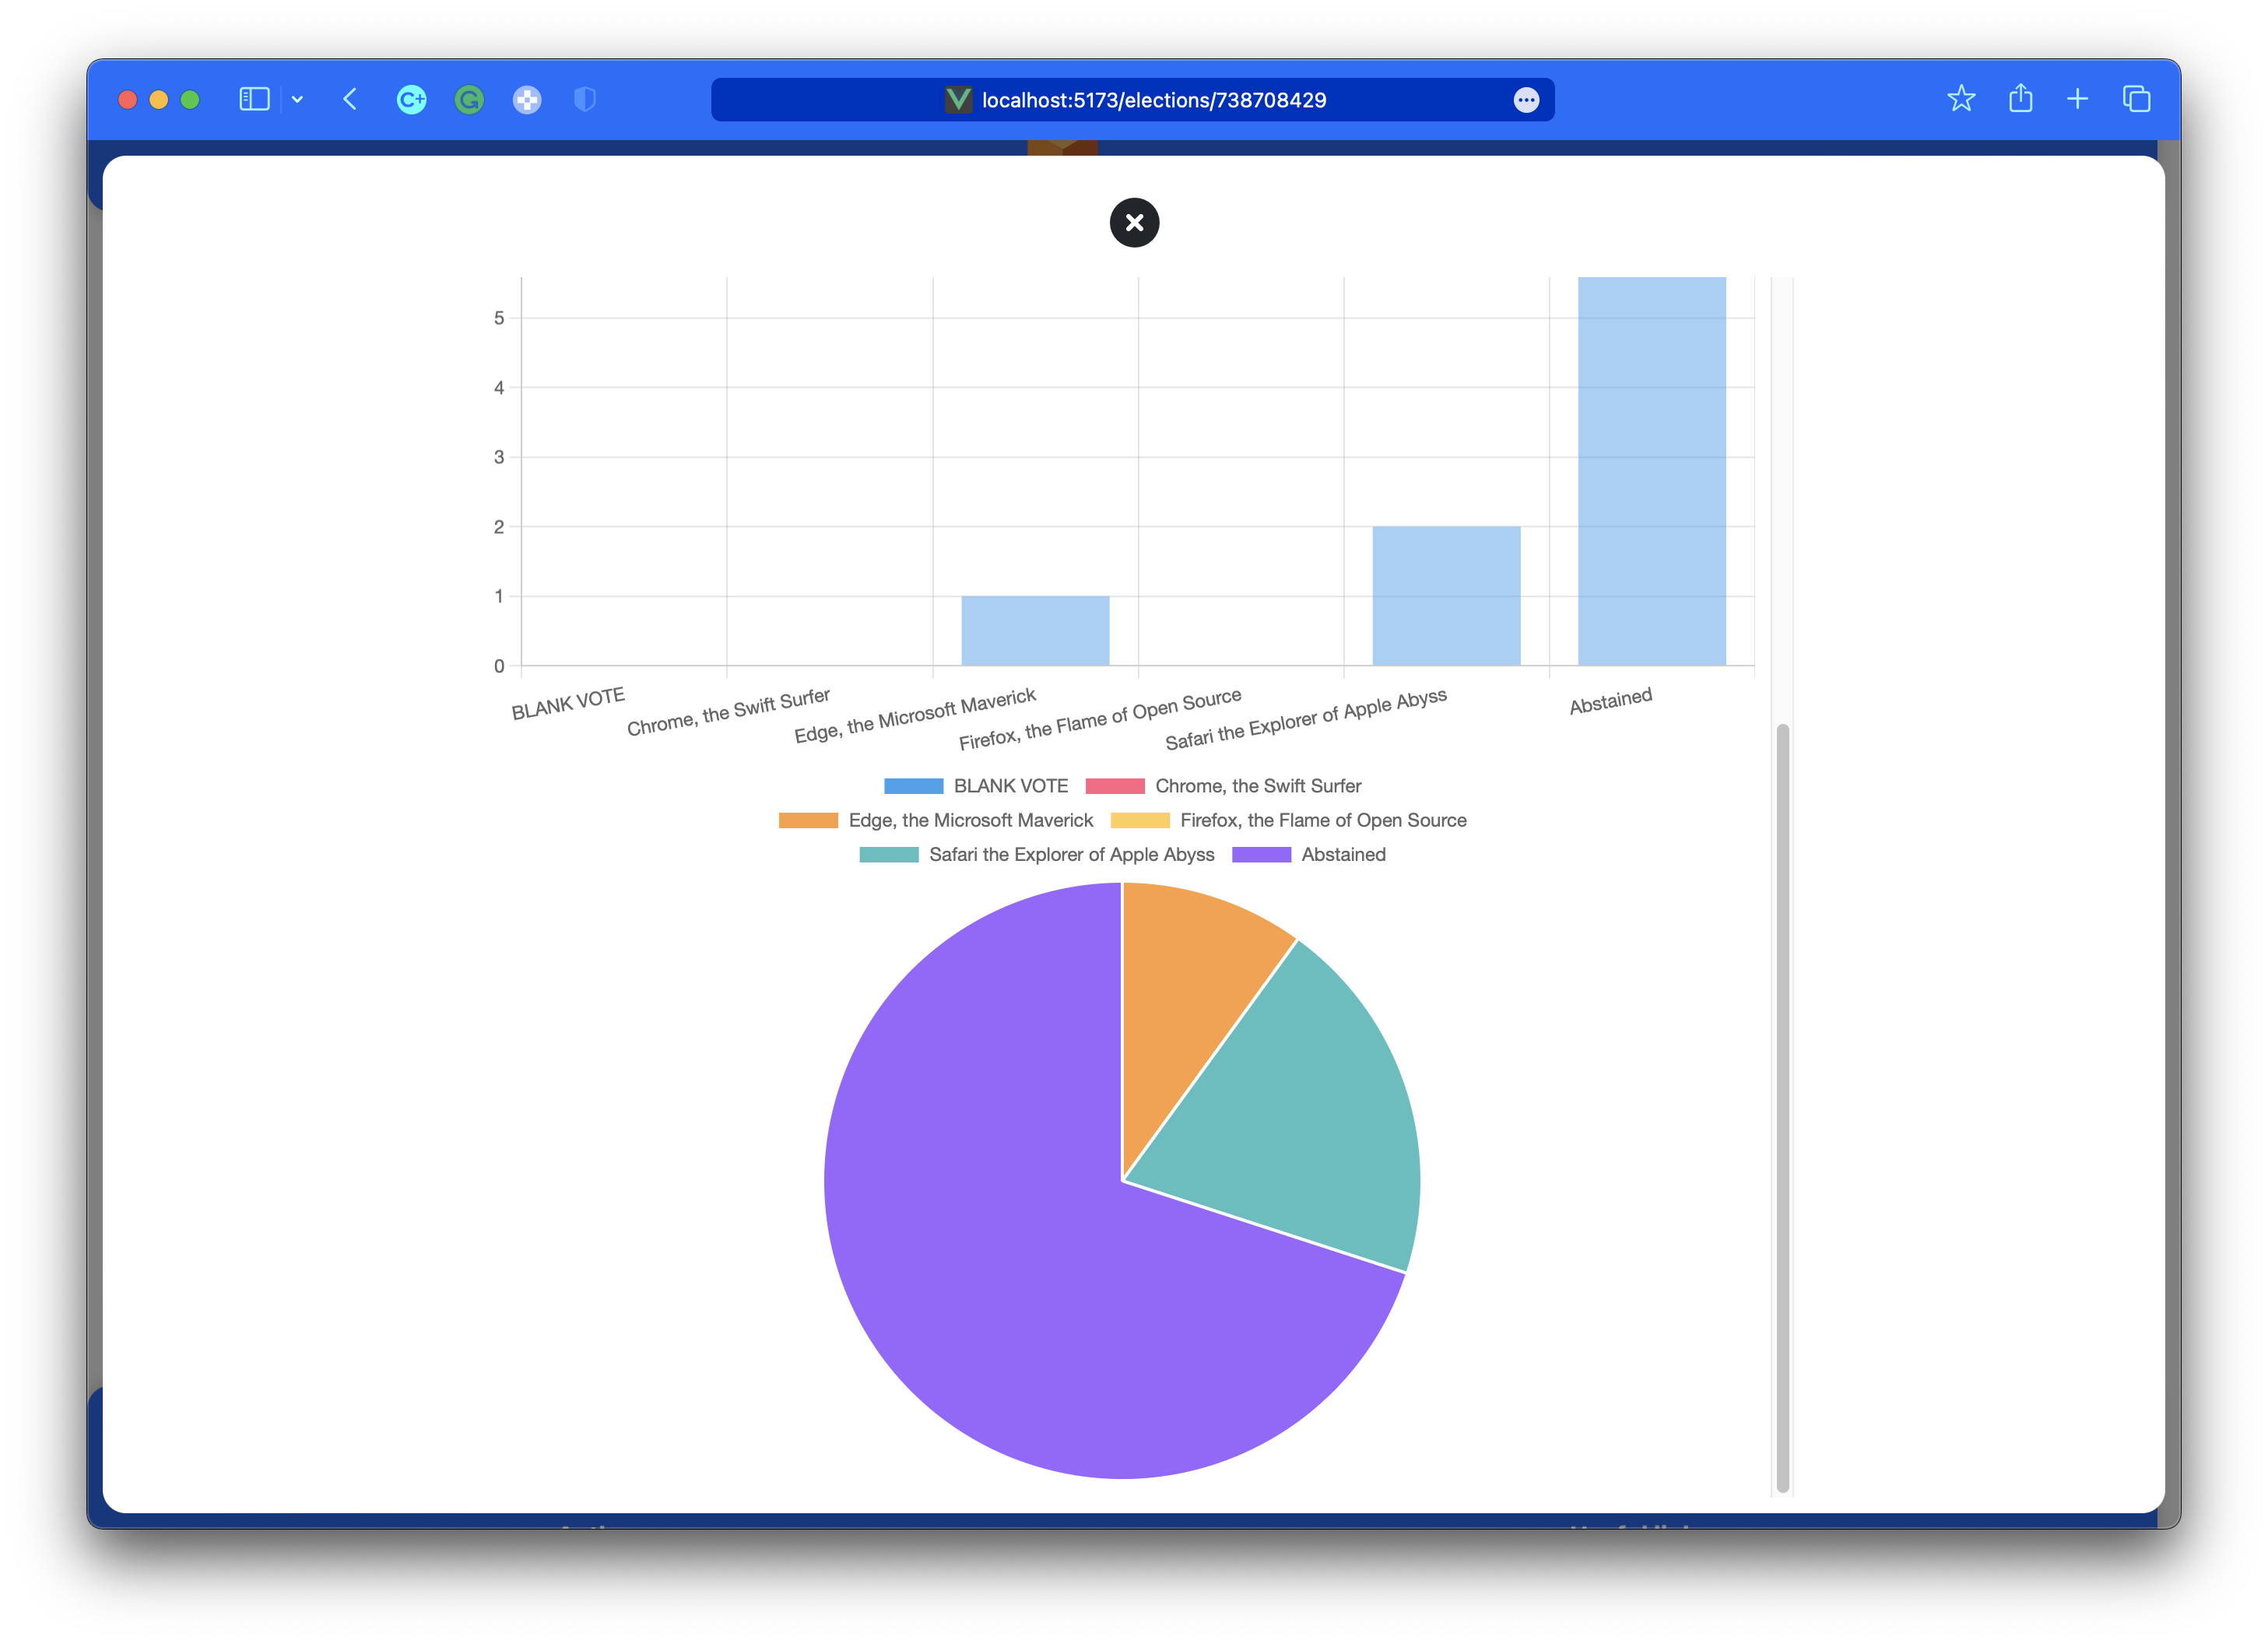
\includegraphics[width=0.9\linewidth]{figures/story-board/14-results.png}
    \label{fig:results-2}
    \caption{Election results view: pie chart.}
\end{figure}

\begin{figure}
    \centering
    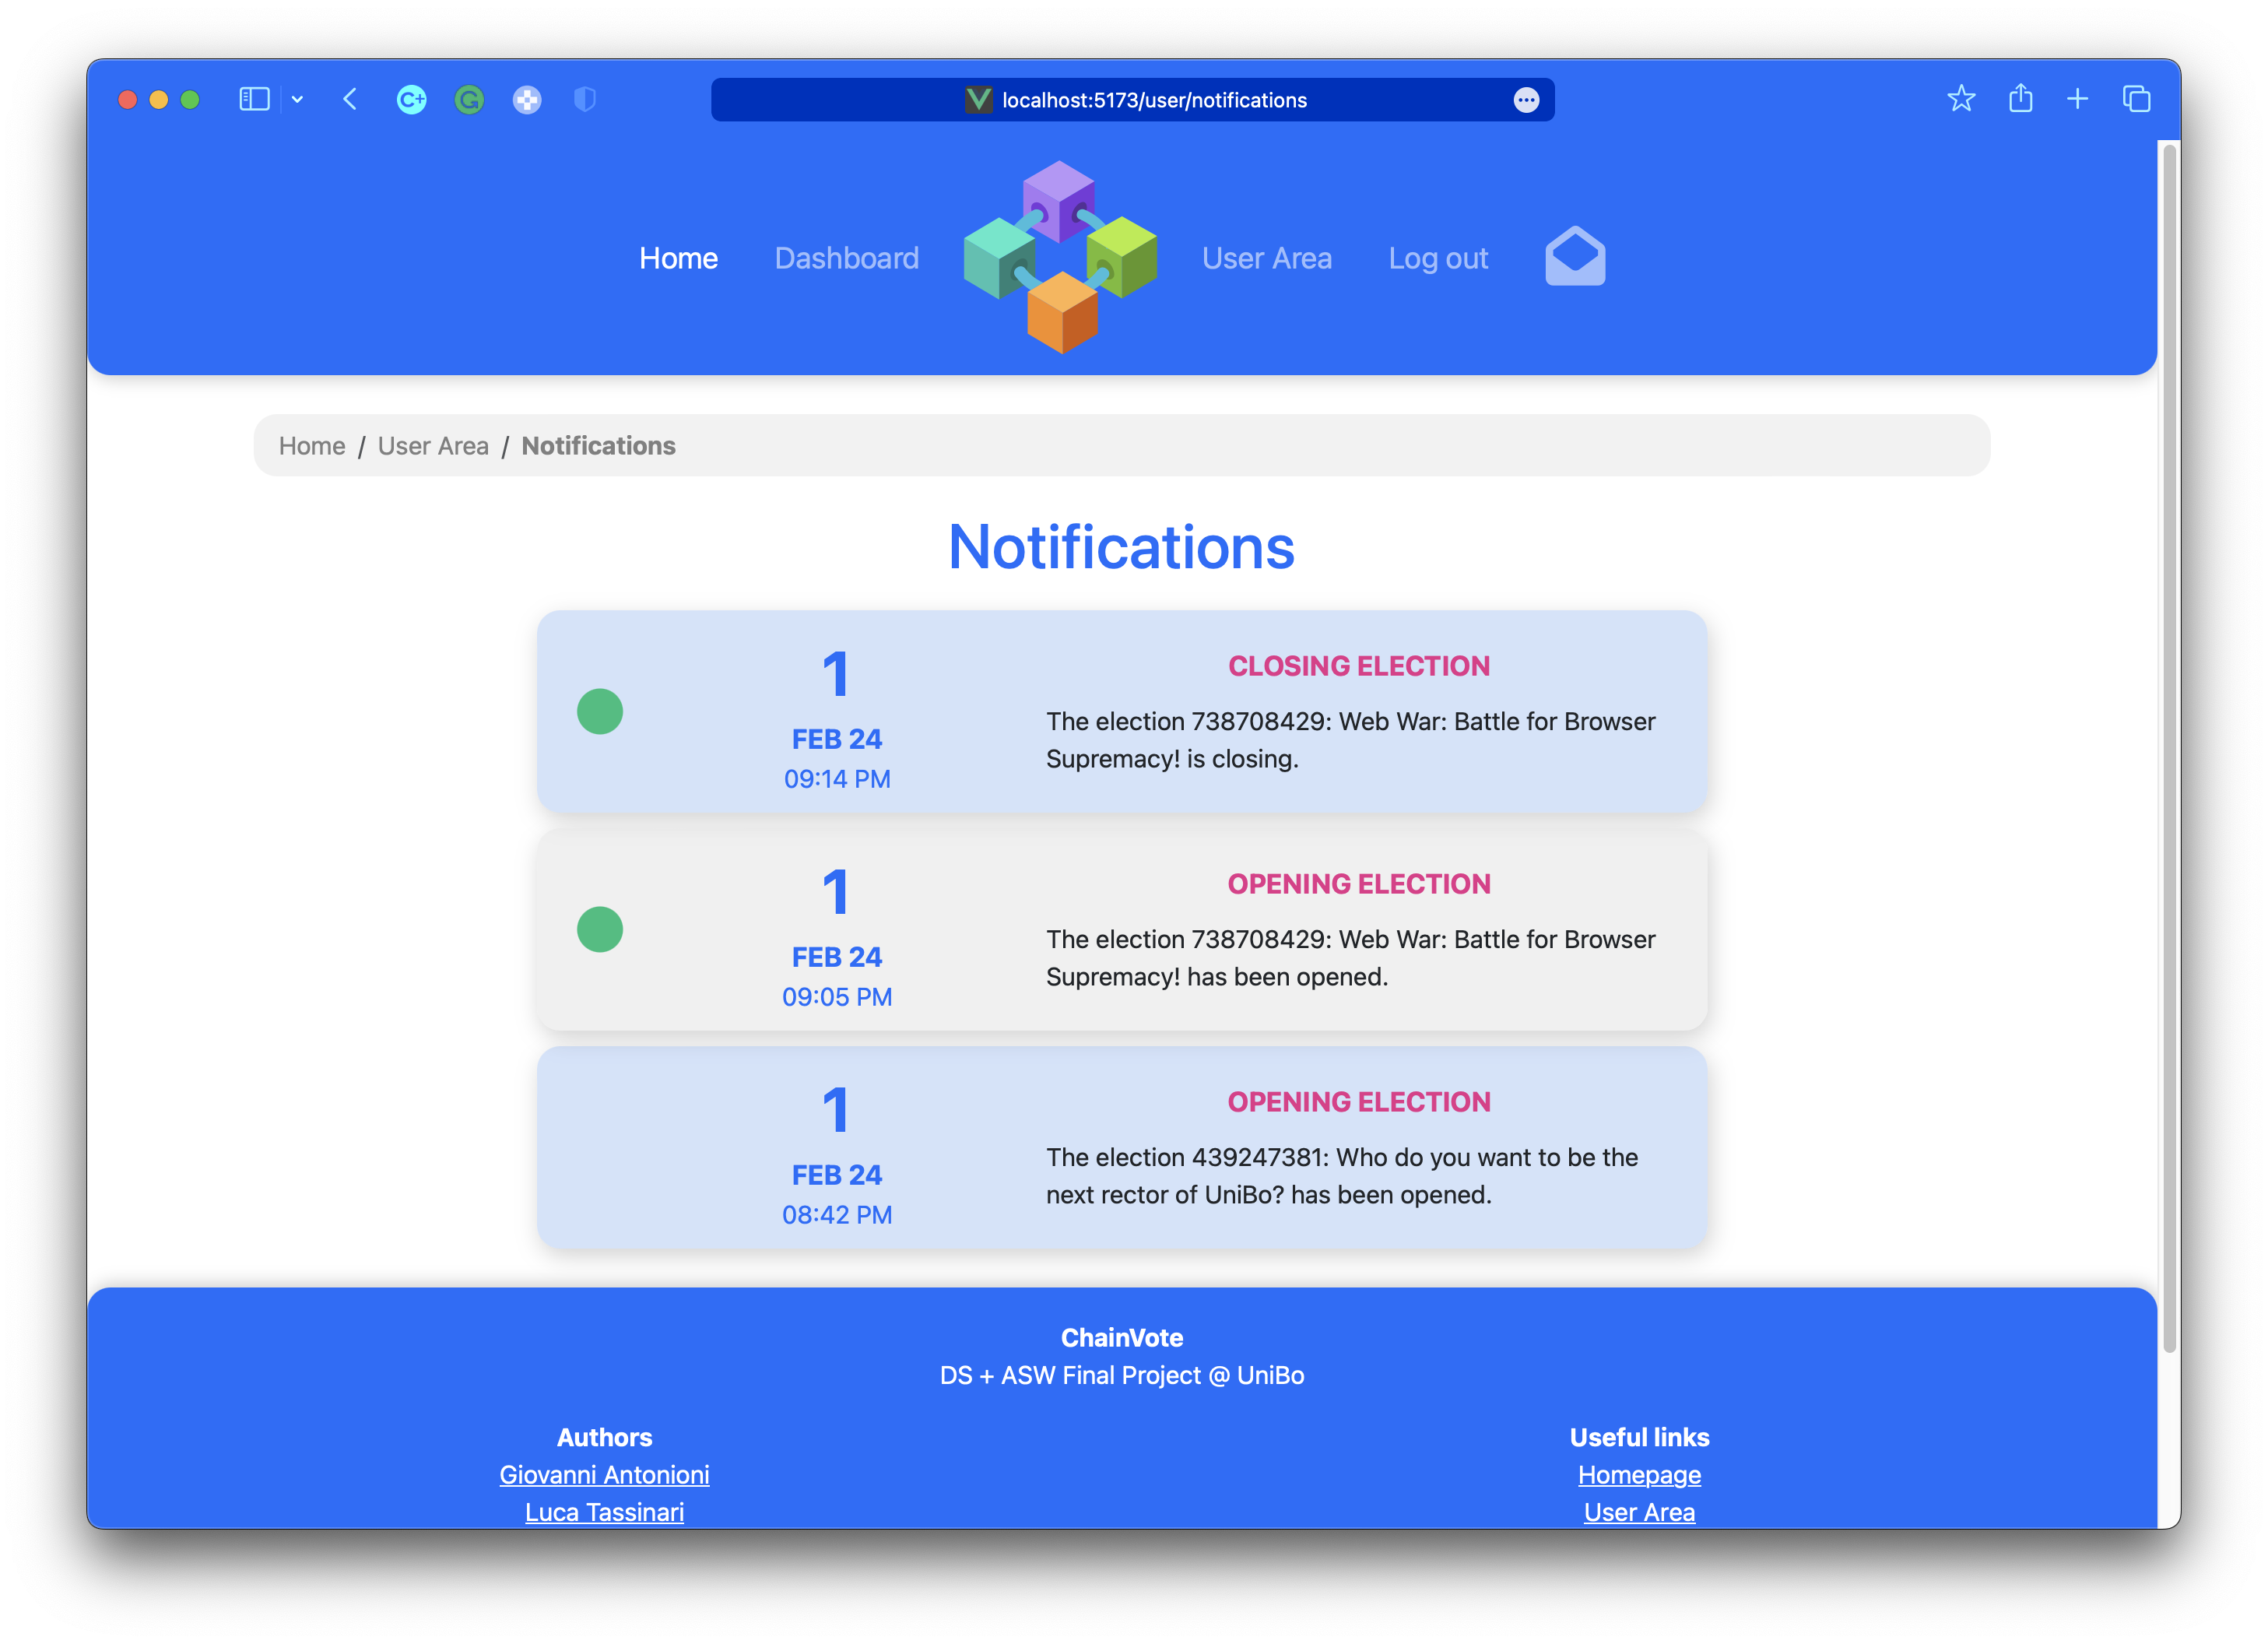
\includegraphics[width=0.9\linewidth]{figures/story-board/15-notifications.png}
    \caption{Notifications list view.}
    \label{fig:notifications-list}
\end{figure}
\restoregeometry

\section{Validation}

Due to mobile first principles, validation phase consisted first of all in testing all the system functionalities by means of browser's mobile visualizer simulator.
This phase has been repeated changing browsers to test portability too. In addition, all the APIs has been tested using either web application, \texttt{Postman} and \texttt{jest}.

\subsection{User experience}

In order to enhance usability and user-experience, Nielsen's heuristics has been considered during the whole development of the system, in details
\begin{itemize}
    \item Visibility of system status, sharing system's status with the user, i.e. during form submission a spinner will report the computation;
    \item Match between system and real world, adopting icons and names familiar with the catchment area;
    \item User control and freedom, in fact the system will never impose an action, but suggest the path the user can follow;
    \item Error prevention, for instance in place of asking for a code, the pop-up raised to display half of a code won't accidentally close;
    \item Recognition rather than recall, since the system has been designed to be the most intuitive as possible;
    \item Minimalist design, adhering to KISS principle, views are designed as minimal but effective;
    \item Help user recognize, diagnose and recover from errors, exposing clear and meaningful messages in place of errors raised.
\end{itemize}

%% -------------------------------------- DS ----------------------------
\iffalse

Tests have been conducted on different levels: domain model, smart contracts and API interactions.

Concerning the domain model of the smart contract unit test has been used (using JUnit framework \cite{junit}).
%
They can be found in \texttt{:core} module.

To test smart contracts, since their functioning requires the network to be up and running, and to effectively bring up the network requires a non-negligible time which would have made the testing environment viscous, Mockito framework \cite{mockito} has been adopted to mock the network-dependent parts.
%
Indeed, Mockito allows the creation of mock objects, which essentially are placeholders for real objects that simulate their behavior by defining the expected outcome provided by specified methods, and spy objects which allow a partial mock of some method of an existing object, retaining its original behavior while customizing certain aspects.
%
An example of usage for the 

\javaimport[
    caption={An example of Mockito behavior definition},
    label={lst:mockito-example}
]{listings/MockitoExample.java}

\javaimport[
    caption={An example of Mockito Spy behavior definition},
    label={lst:mockito-spy-examlpe}
]{listings/MockitoSpyExample.java}

Some testing metrics regarding \texttt{smart-contracts module}: a total of 86 tests were developed, including \texttt{core}, \texttt{presentation} and \texttt{chaincode*} submodules, and the test coverage is overall higher than 80\% (the detail is shown in \Cref{fig:smart-contracts-coverage}).

\begin{info}[\textit{Tests}]
    To run the smart contracts tests, simply: \texttt{./gradlew test} inside the \\ \texttt{smart-contracts} folder of the project.
    \\
    Reports are available in each \texttt{build/reports/tests} submodule directory.
\end{info}

\begin{figure}
    \centering
    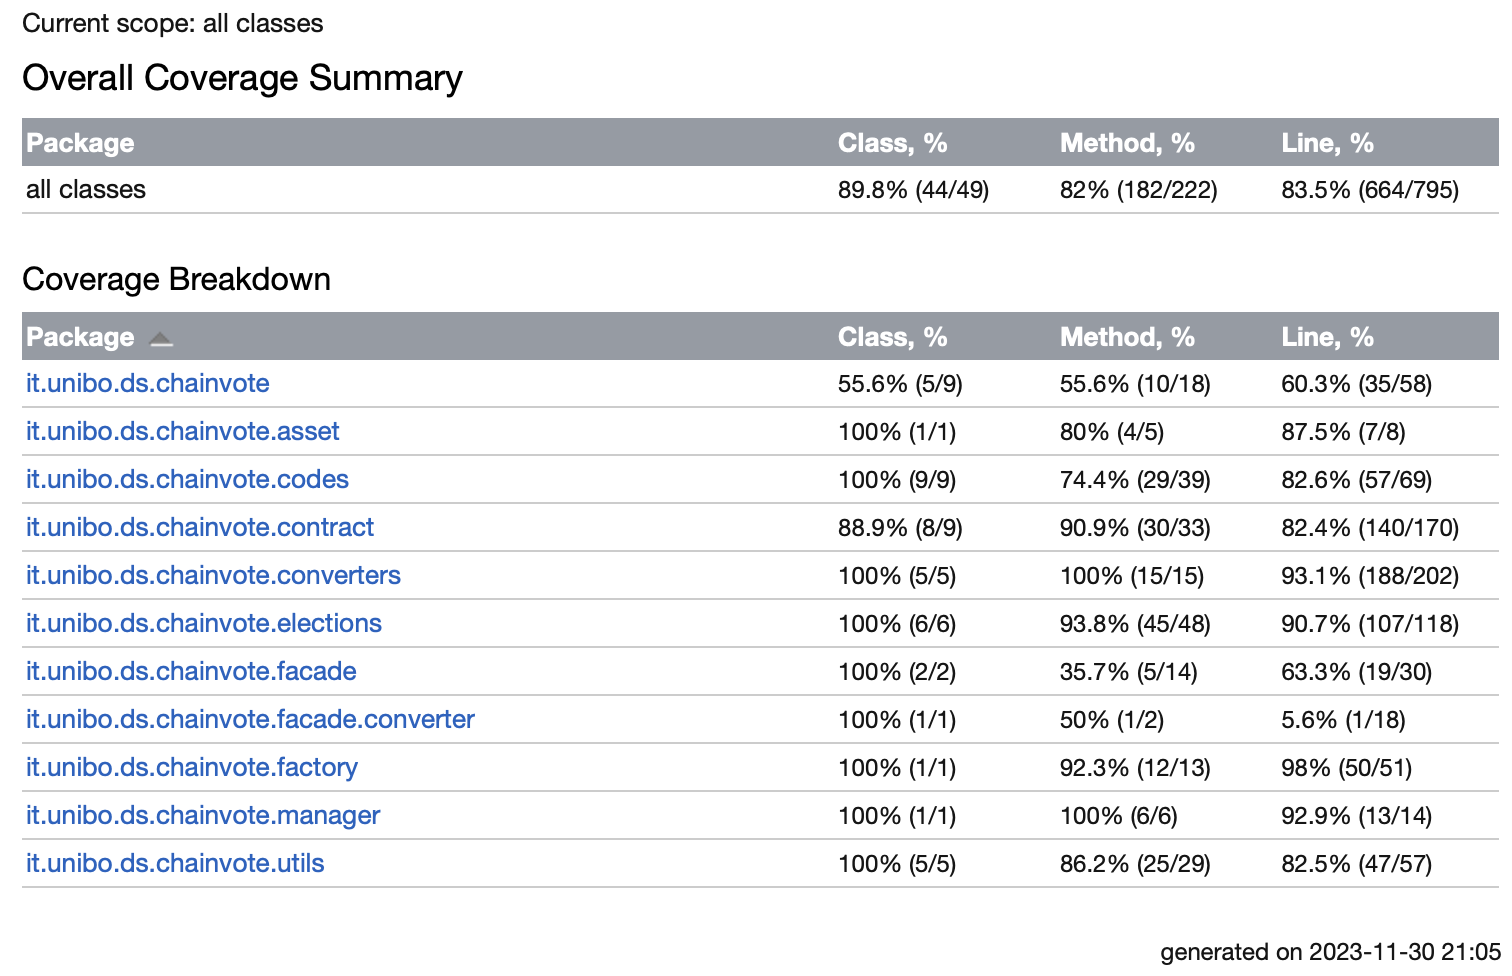
\includegraphics[width=\linewidth]{figures/smart-contracts-coverage.png}
    \caption{Coverage of the \texttt{:smart-contracts} module.}
    \label{fig:smart-contracts-coverage} 
\end{figure}

Concerning distributed quality attributes of the blockchain component, such as fault tolerance, we leverage the Hyperledger Fabric framework which ensures that, for example, if a peer is down, the transactions are redirected to the other peers of the organization.
%
Manual tests have been conducted to stress the network in corner cases (like the one cited above) operating on the peers' containers.

\subsection{API Testing}
The principal goal of the API testing is to verify that the server correctly handles the requests that it receives from the client. To achieve this we used in combination the \texttt{jest} testing library along with \texttt{supertest}. The first one is a JavaScript testing framework that allows the creation of unit tests for JavaScript code, while the latter is a library that allows the creation of HTTP requests to a server

\jsimport[
    caption={An example of an API test},
    label={lst:jest-test}
]{listings/jest.example.ts}

In \Cref{lst:jest-test} we show an example of testing on POST requests to the /code endpoint of the API server. \texttt {jest} allows control division \& execution of the tests introducing initialization and cleanup functions that will be executed before and after the execution of the tests. 
We can group up tests with \texttt{describe} functions, so we can better organize them among the various scenarios of the specific endpoints.
\texttt{request} is a function provided by the \texttt{supertest} library that allows the creation of HTTP requests to a server. It takes as input an instance of the express application, then we can configure it specifying the type of the request and the various parameters.

We check the validity of the response by evaluating the status code and the body of the response. 

\fi
%% -------------------------------------- DS ----------------------------

\section{Deployment}

\subsection{Prerequisites}

\begin{itemize}
    \item Unix-like operating system (either macOS or Linux);
    \item Docker and Docker Compose (on Mac OS make sure the file sharing implementation for the container is set to \texttt{osfx (Legacy)} (\texttt{Settings -> General});
    \item Java 11 or higher;
    \item Node.js 18 or higher;
    \item npm.
\end{itemize}

\begin{warn}
    For security reasons the password for using the mailer is not stored in the repository, but it is passed to the container using a docker secret. Before starting up the system, it's necessary to create a password file, at the position defined in the \texttt{secrets} section of the \texttt{docker-compose.yaml} file:
    \begin{verbatim}
    secrets:
        google_api_secret:
            file: ~/secrets/api-pass.txt
    \end{verbatim}

    Is also possible to specify the mail address that will be used to send the emails by changing the \texttt{MAIL\_ADDRESS} environment variable on the \texttt{api-server} service.

    \begin{verbatim}
        environment:
            ...
            - MAIL_USER=chainvote.01@gmail.com
            ...
        \end{verbatim}
\end{warn}

    



\subsection{Startup}

To bring up the blockchain network, deploy the smart contracts on top of the peers, start the API services and the frontend web app you can use the \texttt{services.sh} script on the root of the project.

To bring up all the system's services:

\begin{verbatim}
    ./services up
\end{verbatim}

Since the first time it will pull Hyperledger Fabric binaries and docker images to create blockchain artifacts and start API services, it will take a while to bring up the entire system.

While it reaches the API server creation phase, the script will execute the \texttt{npm login} command; we've preconfigured some default credentials for this purpose, these should be used when the login request is prompted:
\begin{itemize}
    \item username: \texttt{user}
    \item password: \texttt{password}
\end{itemize} 

\begin{warn}
    During the startup phase of the API layer, the script will require the sudo privileges in order to ensure that the \texttt{verdaccio}, \texttt{cache} and \texttt{dbdata} folders have write and read permissions, which are needed on Linux environment.
\end{warn}

The full working system consists of 33 containers (\Cref{fig:containers}): one for each peer and chaincode deployed on it, five containers for the API services and one for the frontend web app.

\begin{figure}[h!]
    \centering
    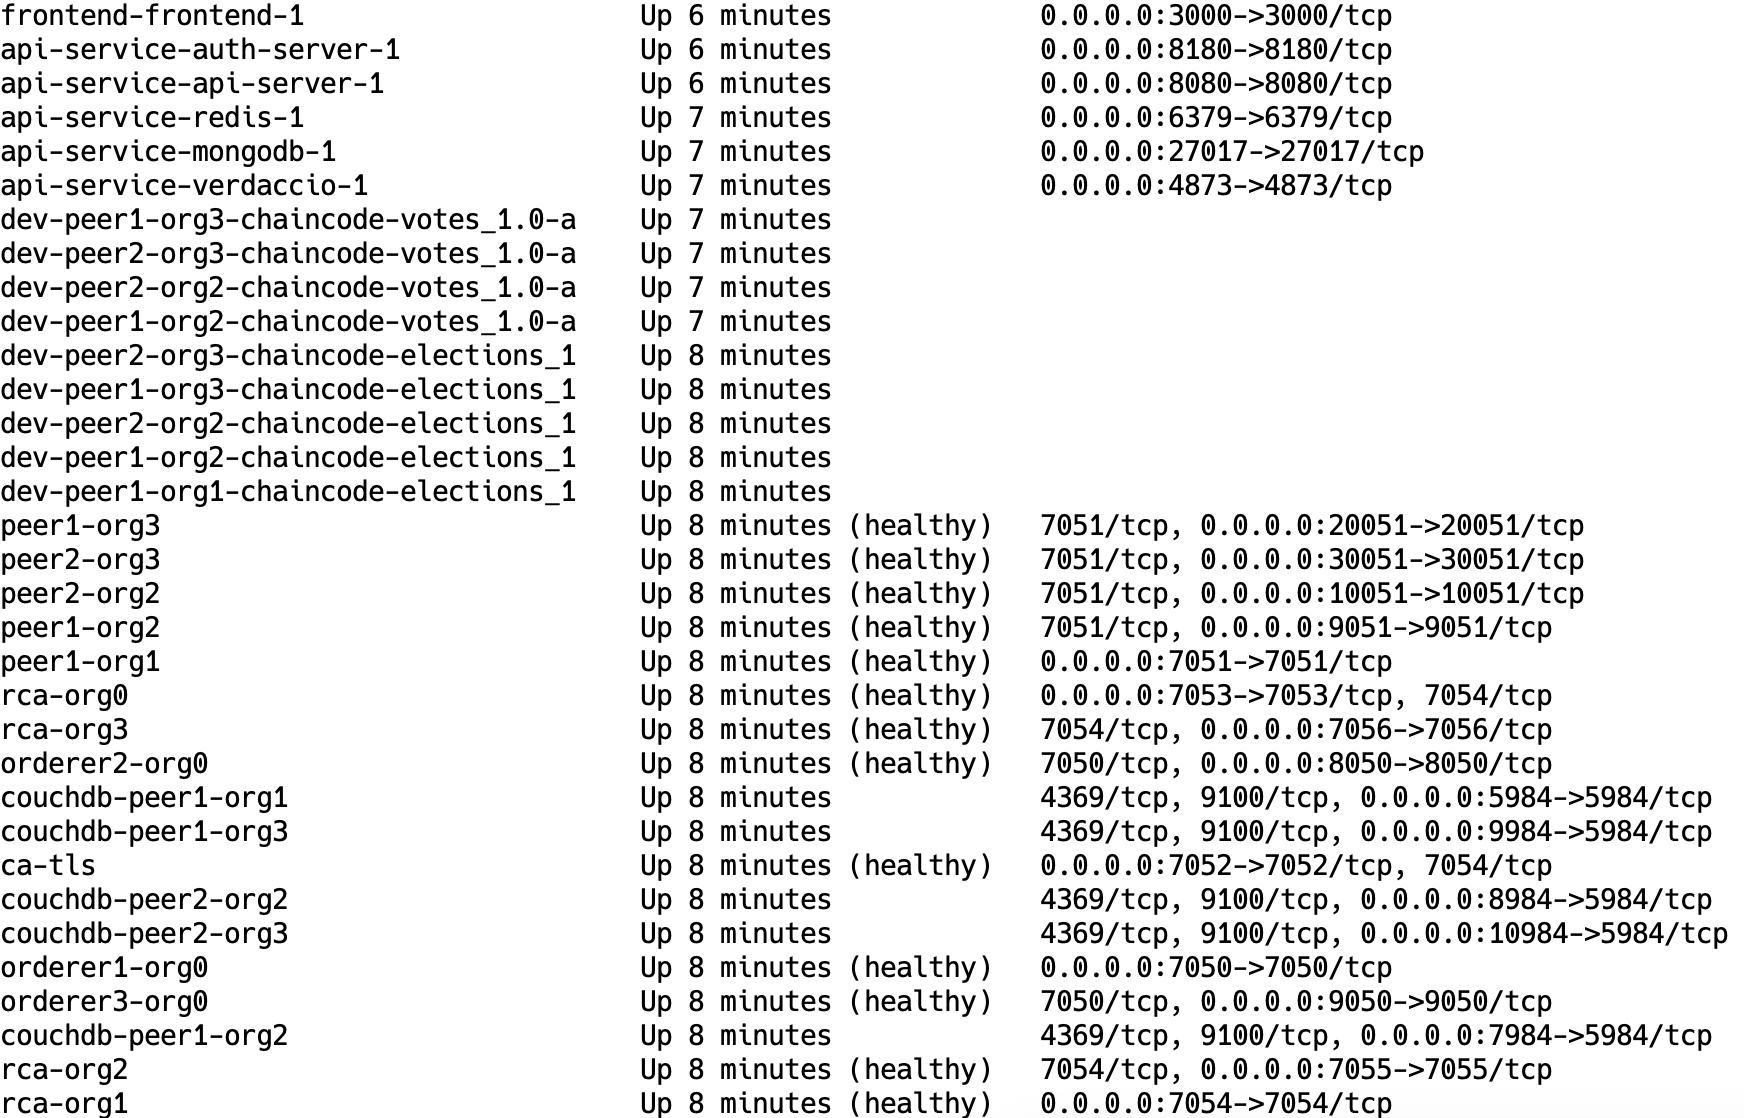
\includegraphics[width=\linewidth]{figures/containers.png}
    \caption{The set of containers that should be up and running at the end of the deployment.}
    \label{fig:containers} 
\end{figure}

To bring them down without cleaning the blockchain artifacts (it will speed up the creation of the network next times):

\begin{verbatim}
    ./services down
\end{verbatim}

To clean network artifacts:

\begin{verbatim}
    ./services clean
\end{verbatim}

%% -------------------------------------- DS ----------------------------
\iffalse

\subsection{Details}
\label{deployment-details}

Each project's module is shipped with a script that automatizes its subpart of the system.
%
\texttt{services.sh} script, under the hood, sequentially executes each module's deployment script in order to make the deployment of the entire system simpler.

\subsubsection*{\texttt{:blockchain} module}

For this module a \texttt{network.sh} bash script automatize the deployment of the blockchain network and all its component.
%
It has been built following the Fabric CA Operations Guide \cite{hyperledger-fabric-ca-docs} \cite{fabric-ca-rework}, simulating its deployment using Docker.

The overall process is non-trivial and it is summarized in \Cref{fig:blockchain-up-sequence}.

\begin{figure}
    \centering
    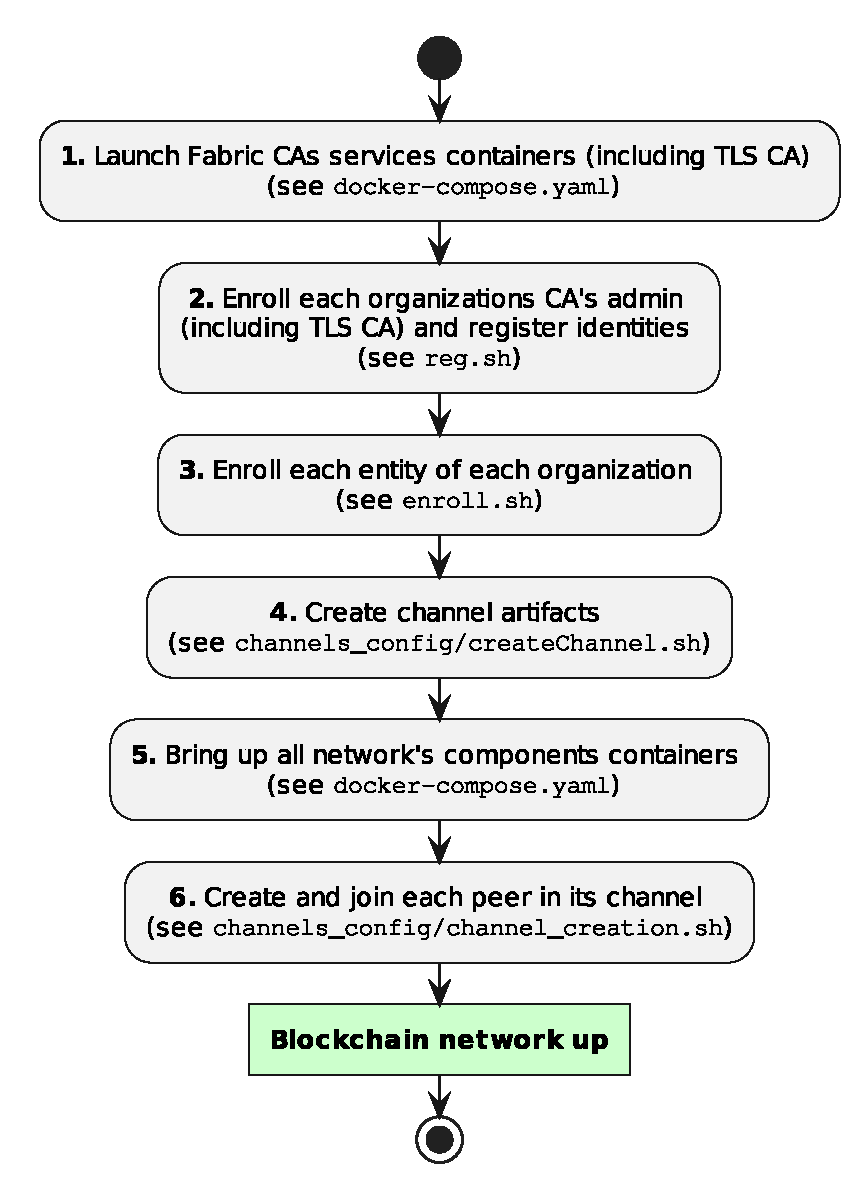
\includegraphics[width=0.6\linewidth]{figures/blockchain-up-sequence.eps}
    \caption{A sequence diagram representing the steps required to create the blockchain network.}
    \label{fig:blockchain-up-sequence}
\end{figure}

After bringing up all the CA's service containers, including the TLS-CA one, (step 1) for each of them an admin is enrolled using the \texttt{fabric-ca-client} script of Hyperledger Fabric.
%
This admin is used to register each entity into the CA database, which will be used in subsequent steps during the enrollment of these entities.
%
These procedures are executed within the \texttt{reg.sh} script (step 2).
%
The enrollment of each entity (both network components and users) from the Certificate Authorities (CAs) is now undertaken for each organization in \texttt{enroll.sh} (step 3).
%
Then, the channel artifacts are generated (step 4) using the \texttt{configtxgen} script provided by Hyperledger Fabric from the configuration files described in \Cref{sec:blockchain-network-impl}.
%
Once the channel artifacts have been created all the network components containers are brought up, the channel is created and peers join them (steps 5 and 6).

All the network components containers are deployed through Docker Compose (using the \texttt{docker-compose.yaml} file in the \texttt{:blockchain} module folder).

\subsubsection*{\texttt{:smart-contracts} module}

The \texttt{:smart-contract} module provides a set of Gradle tasks created to bring up the network, package the chaincodes and install them on the peers.
%
These are shown below (to list them: \texttt{./gradlew tasks}):

\begin{verbatim}
    Blockchain tasks
    ----------------
    cleanAllPackages - Remove all generated packages
    downNetwork - Bring down the blockchain network without cleaning
                  artifacts
    downNetworkAndClean - Bring down the blockchain network and clean
                          the artifacts
    packageChaincodes - Build and generate chaincodes packages
    upAndDeploy - Up the network and deploy chaincodes in one shot
    upNetwork - Bring up the blockchain network
\end{verbatim}

Among others, \texttt{upAndDeploy} is the Gradle task which automatizes the upping of the network and the installation of both chaincodes in one single shot.

Technically, the installation of a chaincode on peers involves, after creating the network, the following steps (\Cref{fig:sc-installation-sequence.eps}):

\begin{enumerate}
    \item Build and generate chaincodes jars;
    \item Package the jars into a \texttt{.tar.gz} files with the \texttt{peer lifecycle chaincode package} command;
    \item Install the chaincodes on every peer that will endorse a transaction with the \texttt{peer lifecycle chaincode install} command;
    \item After the installation, the organization's approval is needed. The set of channel members who need to approve a chaincode before it can be deployed is governed by the \texttt{Application/Channel/LifecycleEndorsement} policy described in \Cref{sec:blockchain-network-impl};
    \item After a sufficient number of organizations have approved a chaincode definition, one organization can commit the chaincode definition to the channel using the \texttt{peer lifecycle chaincode commit} command.
\end{enumerate}

\begin{figure}
    \centering
    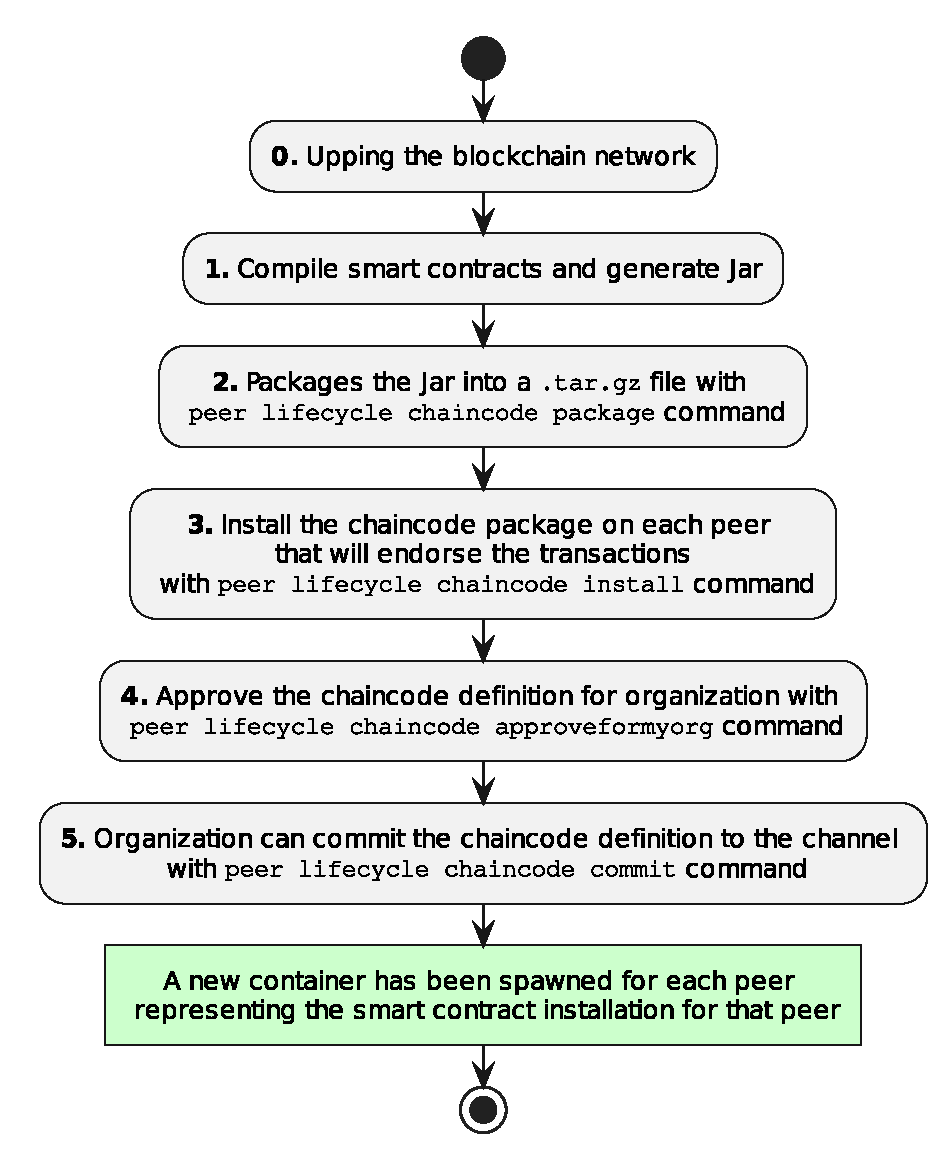
\includegraphics[width=0.7\linewidth]{figures/sc-installation-sequence.eps}
    \caption{A sequence diagram representing the steps required to install the chaincodes on top of the peers.}
    \label{fig:sc-installation-sequence.eps}
\end{figure}

All of these steps have been programmed in Kotlin within Gradle tasks into the \texttt{build.gradle.kts} project's build file.

Moreover, since the startup of the network and the chaincodes installation is a very critical asset for the project a CI Pipeline has been set up to test its functioning at every pushed commit on a \href{https://github.com/tassiLuca/ChainVote}{mirrored repository} hosted on GitHub.

\subsubsection*{\texttt{:api-service} module}

We deploy all the services inside the \texttt{:api-service} module using a simple script called \texttt{startup.sh}. This contains two functions: 
\begin{itemize}
    \item \texttt{up} which will prepare the environment and start the API servers;
    \item \texttt{down} which will stop the API layer.
\end{itemize} 

When the \texttt{up} is executed it will first copy a pair of test keys inside the \texttt{common},\texttt{auth},\texttt{api} folders, these are used for testing the jwt functions. 
After that it creates the data folders that should be used as mounting points for verdaccio and redis: \texttt{dbdata} and \texttt{cache}. 
After that, using the docker-compose yaml file, the \texttt{Verdaccio} server will be started and the common dependencies, inside the \texttt{:common} package will be built and published on the local registry.
Once the dependencies are published the rest of the services are built and started. The \texttt{down} function will simply stop the API layer using the \texttt{docker-compose down} function.

\subsubsection*{\texttt{:frontend} module}

The \texttt{:frontend} module contains just a \texttt{docker-compose.yaml} file thanks to which, simply with \texttt{docker compose up}, the frontend container can be started, listening on port \texttt{3000}.

\fi
%% -------------------------------------- DS ----------------------------

\subsection{Troubleshooting}
If you are encountering issues or observing unexpected behavior during the deployment, this troubleshooting guide is designed to assist you in identifying and resolving common problems.

\subsubsection*{Linux/MacOS: \texttt{[common.tools.configtxgen] main -> Error on outputBlock: could not create bootstrapper: could not create channel group ...: open /Projects/distributed-systems/ds-project/chain-vote/blockchain/ \\../.chainvote/blockchain/org0/orderer1/tls-msp/signcerts/cert.pem: no such file or directory}}

A similar error occurs the next time a problem arises during the creation of channel artifacts because it tries to get some files inside the artifacts folder but, since the previous deployment failed, those files don't exist.
%
Cleaning the artifacts with \texttt{./services clean} should solve the problem.

\subsubsection*{MacOS: resource management}
On MacOS systems make sure to increase allocated resources in Docker Desktop, particularly for CPU and memory limit (8GBs are enough).

\subsubsection*{MacOS: \texttt{Error response from daemon: cannot stop container: <container-id>: tried to kill container, but did not receive an exit event}}

Sometimes happens that, when the services are torn down (with \texttt{./services down} or \texttt{services clean}), one Hyperledger CA container remains hanging.
Restarting Docker Desktop solves this issue.

\subsubsection*{MacOS: \texttt{container peer1-org2 is unhealthy}}
If, during the deployment of the network, the shown message (or a similar one) appears on a MacOS host, make sure the file-sharing implementation for the containers in \texttt{Settings -> General} is set to \texttt{osxfs (Legacy)}.

\subsubsection*{MacOS/Linux: \texttt{General build failure}}
While the system is starting up docker will cache lots of data that is used in the various building phases. This could lead to a general build failure in future runs. Is possible to try these solutions for solving the problems:
\begin{itemize}
    \item \texttt{docker builder prune} to clean the docker cache;
    \item Delete dangling images and volumes;
    \item Restart docker engine;
\end{itemize}

\section{Conclusions}

In this project we designed and implemented a web application that allows a user to interact with our system.

Following the REST API principles and guidelines learned during the lessons, we achieved a good level of usability and user experience, enhancing our technical knowledge about modern web frameworks and tools while, at the same time, getting in touch with real-time scenarios.

Despite being a challenging project we can consider reached our fixed goals, fulfilling all the requirements of the system.


\nocite{*} % Includes all references from the `references.bib` file
\bibliographystyle{plain}
\bibliography{references}

\end{document}
